\documentclass[letterpaper,10pt]{article}
\usepackage[letterpaper, hmargin=1.8cm, vmargin = 2.5cm]{geometry} %Sets the page geometry
\usepackage{url}
\usepackage{hyperref}

\usepackage{multicol}
\setlength{\columnsep}{1cm}
\setlength{\columnseprule}{0.7pt}

\usepackage[english]{babel}
\usepackage{datetime2}

\usepackage{setspace}
\setlength{\parskip}{1em} % Set space when paragraphs are used
\setlength{\parindent}{0in}

\usepackage{xcolor}
\usepackage{multicol}
\usepackage{float}
\usepackage{graphicx} % Package for \includegraphics
\usepackage{wrapfig} % Figure wrapping
\usepackage[T1]{fontenc} % Output font encoding for international characters
\usepackage{amssymb}
\usepackage{amsmath}
\numberwithin{equation}{section}
%%%%% Boxes Setup %%%%%
\usepackage[many]{tcolorbox}    	% for COLORED BOXES (tikz and xcolor included)
\definecolor{main}{HTML}{dedcdc}    % setting main color to be used
\definecolor{sub}{HTML}{dedcdc}     % setting sub color to be used
\definecolor{main2}{HTML}{a9b8de}    % setting main color to be used
\definecolor{sub2}{HTML}{a9b8de}     % setting sub color to be used

\tcbset{
    sharp corners,
    colback = white,
    before skip = 0.3cm,    % add extra space before the box
    after skip = 0.3cm      % add extra space after the box
}                           % setting global options for tcolorbox
\newtcolorbox{boxD}{
    colback = sub, 
    colframe = main, 
    boxrule = 0pt, 
    toprule = 0pt, % top rule weight
    bottomrule = 0pt % bottom rule weight
}

\newtcolorbox{boxE}{
    colback = main2, 
    colframe = sub2, 
    boxrule = 0pt, 
    toprule = 0pt, % top rule weight
    bottomrule = 0pt % bottom rule weight
}

\usepackage{amsthm}
\usepackage{mathtools}
\usepackage{thmtools}
\usepackage{bbm}
\usepackage[autostyle]{csquotes}
\usepackage{doi}
\usepackage[
    backend=biber,
    style=authoryear-comp,
    natbib=true,
    sorting=nyt,
    oi=false,
    isbn=false,
    url=false,
    eprint=false,
    sortlocale=en_US,
    url=false, 
    doi=true,
    eprint=false
]{biblatex}

\AtEveryBibitem{\clearfield{note}\clearfield{addendum}}
\AtEveryCitekey{\clearfield{note}\clearfield{addendum}}

\addbibresource{bibliography.bib}

% Other
\newtheorem{thm}{Theorem}
\numberwithin{thm}{section}
\newtheorem{dfn}{Definition}
\newtheorem{lem}{Lemma}
\numberwithin{lem}{section}
\newtheorem{rmk}{Remark}
\newtheorem{exmp}{Example}
\newtheorem{cor}{Corollary}
\numberwithin{cor}{section}
% \newtheorem{prop}{Proposition}
\newtheorem{asm}{Assumption}

\renewcommand\qedsymbol{$\blacksquare$}

\newcommand{\sumi}{\sum_{i=1}^n}
\newcommand{\calE}{\mathcal{E}}
\makeatother
\renewcommand{\hat}{\widehat}
\newcommand{\E}{\mathbb{E}}
\newcommand{\1}{\mathbbm{1}}
\newcommand{\Var}{\text{Var}}
\newcommand{\Cov}{\text{Cov}}
\newcommand{\rk}{\text{rk}}
\renewcommand{\P}{\mathbbm{P}}

\makeatletter
\def\blfootnote{\gdef\@thefnmark{}\@footnotetext}
\makeatother

\DeclarePairedDelimiter\floor{\lfloor}{\rfloor} %Floor function
\DeclarePairedDelimiter\ceil{\lceil}{\rceil} %Ceil function
\DeclareMathOperator*{\argmax}{arg\,max} % argmax
\DeclareMathOperator*{\argmin}{arg\,min} % argmin
\newcommand{\indep}{\perp\!\!\!\!\perp} 


\begin{document}
\singlespacing
\title{Inference for Conditional Average Treatment Effects using \\ Distributional Nearest Neighbors}
\date{Last edited: \DTMtoday}
\author{Jakob R. Juergens \\ University of Wisconsin - Madison}
\maketitle
\hrule
\onehalfspacing
\begin{abstract}
    This paper presents a novel method for estimating heterogeneous treatment effects based on a weighted nearest-neighbor estimator.
    As part of this analysis, for a class of generalized U-statistics, I improve on conditions currently available in the literature required for consistent variance estimation.
    Furthermore, I provide corresponding results for asymptotically valid pointwise inference in a nonparametric regression setup.
    I extend the ideas of this nonparametric regression estimator to the estimation of conditional average treatment effects using ideas from double / debiased machine learning including Neyman-orthogonal moments and cross-fitting.
    This results in a nonparametrically weighted DDML variant that is new to the literature and resembles recent kernel-based approaches under a data-adaptive kernel.
    Corresponding variance estimation results are provided that allow for asymptotically valid inference.
    \blfootnote{The author thanks Jack Porter and Harold D. Chiang for their invaluable feedback.}
\end{abstract}
\vspace{0.3cm}
\hrule
\singlespacing

\vspace{-0.3cm}
\begin{center}
    {\small Supplementary Material and R-Package available at: \url{https://github.com/JakobJuergens/Unif_Inf_TDNN}}
\end{center}
\vspace{0.3cm}
\hrule
\singlespacing
\thispagestyle{empty}

\pagenumbering{arabic}
\onehalfspacing

\newpage
    \begin{multicols*}{2}
        {\small \tableofcontents}
    \end{multicols*}

\newpage
\section{Introduction}
\hrule
Nearest-Neighbor type estimators and their derivatives are a popular class of estimators that is frequently used in fields such as Computer Science or Economics.
However, the development of inferential theory for these estimators is not yet up to par with their widespread adoption in practice.
One such estimator with a particularly close connection to random forests (RF) is the ``two-scale distributional nearest neighbor estimator'' (TDNN) of \citet{demirkaya_optimal_2024}.
In the aforementioned paper, the authors develop a novel debiasing method that promises great improvements on the finite sample properties of the estimator and show its asymptotic normality.
The main contributions of this paper are twofold.
First, this paper provides extended consistency results for the variance estimators for the DNN and TDNN estimators.
These results show consistency for three Jackknife-based variance estimators in a broad class of asymptotically Gaussian generalized U-statistics that extends considerably beyond the DNN-based regression approaches.
Second, I propose a novel estimator for the CATE based on the ideas inherent to the DNN estimator and methods from DDML.
Simulations show promising performance of the estimator, and its simple structure when compared to competing estimators motivates further research into its use for pointwise and simultaneous inference.
These extensions will be at the heart of future iterations of this paper.

After short sections on notation and literature review, the remainder of this paper is organized as follows.
Section~\ref{sec:setup} introduces the two setups covered in this paper: first, a relatively simple nonparametric regression setup and second, a setup that mimics the problem of estimating conditional average treatment effects (CATE).
To give readers a more economic understanding of the ideas presented in this paper, I will also introduce a running example that I will refer to throughout this paper.
This running example will be a simplified version of the well-known problem of estimating treatment effects in a job-training program for individuals of differing characteristics.
Furthermore, this section introduces and contextualizes most of the assumptions that I refer to at later stages of the paper.
Section~\ref{sec:TDNN} is used to define the DNN and TDNN estimators in the context of nonparametric regression and introduces a novel estimator for the CATE setup.
In addition, the main results of the distributional approximations of the estimators are introduced.
Section~\ref{sec:pw_inf} introduces consistency results for variance estimators to allow for pointwise inference using the DNN estimator and its derivatives.
While purely asymptotic in nature, these results improve on currently available results for generalized U-statistics and apply to a broader context than the one presented in this paper.
The future iterations of this paper will then tackle the problem of simultaneous inference using techniques developed by \citet{ritzwoller_simultaneous_2024}.
These novel developments have the potential to significantly extend the applicability of the estimator to scenarios where the treatment effect for a large number of subgroups is of importance.
Section~\ref{sec:simulations} contains multiple simulation experiments that show the performance of the methods presented in this paper in a setting that mimics an economic analysis.
Section~\ref{sec:application} applies the new CATE estimator to {\color{red} LOREM IPSUM}.
Lastly, Section~\ref{sec:conclusion} concludes.

\newpage
\subsection{Notation}
\hrule
Let $[n] = \{1, \dotsc, n\}$.
Given a finite index set $\mathcal{I} \subset \mathbb{N}$, I introduce the following notational conventions.
\begin{equation}
	L_{s}(\mathcal{I}) = \left\{\left(l_1, \dotsc, l_s\right) \in \mathcal{I}^{s} \, \middle| \, l_{1} < l_{2} < \dotsc < l_{s}\right\}
	\quad \text{and} \quad
	L_{n,s} = L_s\left([n]\right)
\end{equation}
For a data set $\mathbf{D}_{[n]} = \left(Z_1, \dotsc, Z_{n}\right)$ and a vector $\ell \in L_{n,s}$, denote by $\mathbf{D}_{[n], -\ell}$ the data set where the observations corresponding to indices in $\ell$ have been removed.
To simplify the notation in the case that a single observation (say the $i'th$ observation) is removed, I use the notation $\mathbf{D}_{n, -i}$.
Similarly, given such a data set $\mathbf{D}_{[n]}$ and index vector $\ell$, denote by $\mathbf{D}_{\ell}$ the data set consisting only of the observations in $\mathbf{D}_{[n]}$ corresponding to the indices in $\ell$.
In an abuse of notation, when considering two index vectors $\ell$ and $\iota$ that do not share any entries, I denote by $\ell \cup \iota$ the concatenation of the two vectors, e.g., if $\ell = (8,2,5)$ and $\iota = (1,6)$, then $\ell \cup \iota = (8,2,5,1,6)$.
In the following, $\rightsquigarrow$ denotes weak convergence, while $\rightarrow_{p}$ denotes convergence in probability, and $\rightarrow_{a.s.}$ denotes almost sure convergence. 
We will use the symbol $\lesssim$ to denote an inequality that holds for sufficiently large sample sizes $n$ or kernel orders $s$. 
As we consider settings where these diverge together, the specific reference parameter will be clear from the context.

\subsection{Related Literature}
\hrule
The related literature can be broadly categorized into three main strands: Nearest-Neighbor type estimators in nonparametric regression, variance estimation for (generalized) U-statistic type estimators including Random Forest, and estimation and inference for CATEs using double / debiased machine learning (DDML) methods.
A great introduction to the Nearest-Neighbor method is given in \citet{biau_lectures_2015}, illustrating the potential of the method for classification and regression tasks.
Of particular interest in the context of this paper are the so-called ``Weighted Nearest-Neighbor'' methods for nonparametric regression.
While this is a well-studied type of estimator in and of itself, I draw particular connections to bagged-nearest-neighbor type estimators.
This class of estimators is built on the framework of ``potential closest neighbors'' as introduced by \citet{lin_random_2006}.
Relevant papers studying their properties are, among others, \citet{biau_rate_2010}, \citet{biau_layered_2010}, and \citet{steele_exact_2009}.
These papers also point out the close connections to RF and illustrate why studying the bagged nearest-neighbor method could potentially guide our analysis of RF.
Recently, \citet{demirkaya_optimal_2024} developed a clever debiasing procedure for the bagged or, as they coin it, distributional nearest-neighbor estimator by combining multiple subsampling scales.
The resulting TDNN estimator lies at the heart of this paper, and the results presented here should be seen in the context of the already established distributional approximations established in the paper.

U-statistics were introduced by Wassily Hoeffding in
\citet{hoeffding_class_1948} and have been a well-established tool in
mathematical statistics for a long time. Thus, there is a significant body of
literature that studies their properties, including outstanding introductions such
as \citet{lee_u-statistics_2019}. Concerning variance estimation for
U-statistics, two highly related papers are \citet{arvesen_jackknifing_1969},
exploring the theory of the Jackknife when applied to U-statistics, and
\citet{arcones_bootstrap_1992} which fulfills a similar role for the bootstrap.
Building on the concept of U-statistics, \citet{peng_rates_2022} introduced the
notion of generalized U-statistics, unifying randomized, incomplete, and
infinite-order U-statistics that have been previously established in the
literature. While being a relatively novel development, there is a significant
body of literature concerning infinite-order U-statistics, which share their
structure with the TDNN estimator. As the purpose of variance estimation in the
problem at hand is ultimately to employ distributional approximations, papers
such as \citet{chen_randomized_2019} and \citet{song_approximating_2019} are
similarly of high relevance for potential applications. Due to the close
connection to the random forest method introduced by
\citet{breiman_random_2001}, there is also a relevant overlap with the
literature on that topic. Thus, articles such as \citet{wager_confidence_2014} and
\citet{wager_estimation_2018} are of special interest, especially since causal forests are considered the state-of-the-art technique for estimating CATEs.

In the context of estimation and inference regarding CATEs using DDML, \citet{chernozhukov_doubledebiased_2018} should be pointed out first.
By combining cross-fitting with the use of Neyman-orthogonal moments, the authors built the foundation for many modern methods for estimation in the presence of high-dimensional nuisance parameters.
Several extensions to this highly influential idea have been proposed, some of which explicitly aim at estimating CATEs.
An example is \citet{semenova_debiased_2021}, who develops estimation and inference procedures for the best linear predictor of a class of causal functions that contain the CATE.
Following a different approach, \citet{chernozhukov_conditional_2024} introduce the concept of conditional influence functions and develop a Kernel-based method that similarly to the paper at hand aims at the nonparametric estimation of causal parameters such as the CATE.
In a similar vein, \citet{chernozhukov_simple_2022} is highly relevant, as it provides a very general analysis of DDML as a meta-algorithm, covering the estimation and inference for CATE.

\section{Setup}\label{sec:setup}
\hrule
Throughout this paper, we will consider two distinct setups focusing on separate but intertwined problems.
As a running example to give immediate economic meaning to the statistical problems, we consider the problem of evaluating a job training program given only observational data in the style of \citet{lalonde_evaluating_1986}.
\begin{boxE}
	\begin{exmp}[Average Hourly Earnings and IT Training]\label{asm:run_exmp}\mbox{}\\*
        Imagine obtaining a large data set containing hourly earnings $Y$ of workers with age $X_1$ and $X_2$ years of education.
        A typical quantity of interest is the average hourly earnings given a specific combination of worker characteristics, for example the average earnings for a 20-year-old worker with 12 years of education (a recent high school graduate without further education).
	\end{exmp}
\end{boxE}
To simplify the presentation, the running example ignores many widely discussed economic problems in this environment and instead focuses on a highly stylized problem with a limited set of characteristics.
The first statistical setup is a pure nonparametric regression setup that closely mirrors the structure of \citet{demirkaya_optimal_2024} and will be useful to illustrate the inner workings of the estimator of interest.
\begin{boxD}
	\begin{asm}[Nonparametric Regression DGP]\label{asm:npr_dgp}\mbox{}\\*
		The observed data consists of an i.i.d.\ sample taking the following form.
		\begin{equation}\label{DGP1}
			\mathbf{D}_n = \{Z_{i} = (X_{i}, Y_{i})\}_{i = 1}^{n}
			\quad \text{from the model} \quad
			Y = \mu(X) + \varepsilon,
		\end{equation}
		where $Y \in \mathbb{R}$ is the response, $X \in \mathcal{X} \subset \mathbb{R}^k$ is a feature vector of fixed dimension $k$ distributed according to a density function $f$ with associated probability measure $\varphi$ on $\mathcal{X}$, and $\mu(x)$ is the unknown mean regression function.
		$\varepsilon$ is the unobservable model error on which we impose the following conditions.
		\begin{equation}
			\E\left[\varepsilon \, \middle| \, X\right] = 0, \quad
			\Var\left(\varepsilon \, \middle| \, X = x\right) = \sigma_{\varepsilon}^2\left(x\right)
		\end{equation}
		Let the distribution induced by this model be denoted by $P$ and thus $Z_{i} = \left(X_{i}, Y_{i}\right) \overset{\text{iid}}{\sim} P$.
	\end{asm}
\end{boxD}
We will also consider a second statistical setting with more immediate econometric relevance: estimation of and inference on heterogeneous treatment effects in the potential outcomes framework.
This statistical setup serves as a more immediately applicable version of the theoretical setup presented in \citet{ritzwoller_simultaneous_2024} and brings their results closer to practitioners in the field of economics.
\begin{boxE}
    \addtocounter{exmp}{-1}
    \begin{exmp}[Average Hourly Earnings and IT Training - continued]\mbox{}\\*
        Consider the introduction of a job training program that covers basic IT skills that potentially influence the average earnings of a worker with given characteristics.
        Think of providing said IT training to a 20-year-old high-school graduate without further education or a 56-year-old with a PhD. It seems unreasonable to expect the effect of basic IT training on hourly wages to be similar in these cases.
        Furthermore, it seems unlikely for these participants to choose to participate in the training with equal probability, adding an additional complicating factor.
    \end{exmp}    
\end{boxE}
\begin{boxD}
	\begin{asm}[Heterogeneous Treatment Effect DGP]\label{asm:CATE_dgp}\mbox{}\\*
		The observed data consists of an i.i.d. sample taking the following form.
		\begin{equation}\label{DGP2}
			\begin{aligned}
				\mathbf{D}_n & = \{Z_{i} = (X_{i}, W_{i}, Y_{i})\}_{i = 1}^{n}
				\quad \text{from the model} \quad
				Y = \1(W = 0)\mu_{0}(X) + \1(W = 1)\mu_1(X) + \varepsilon,	\\
				W_{i} & \sim \operatorname{Bern}\left(\pi\left(X_{i}\right)\right)
			\end{aligned}
		\end{equation}
		where $Y \in \mathbb{R}$ is the response and $W \in \{0,1\}$ is an observed treatment indicator.
		$X \in \mathcal{X} \subset \mathbb{R}^k$ is a vector of covariates of fixed dimension $k$ distributed according to a density function $f$ with an associated probability measure $\varphi$ on $\mathcal{X}$ and $\varepsilon$ is the unobservable model error on which we impose the following conditions.
		\begin{equation}
			\varepsilon \indep W \, | \, X, \quad
			\E\left[\varepsilon \, | \, X\right] = 0, \quad
			\Var\left(\varepsilon \, | \, X = x\right) = \sigma_{\varepsilon}^2\left(x\right)
		\end{equation}
		Furthermore, $\mu_0:\mathcal{X} \rightarrow \mathbb{R}$ and $\mu_1:\mathcal{X} \rightarrow \mathbb{R}$ are the two unknown potential outcome functions and $\pi:\mathcal{X} \rightarrow [0,1]$ is a function describing the probability of treatment uptake, effectively corresponding to the propensity score.
		Let the distribution induced by this model be denoted by $Q$ and thus $Z_{i} = \left(X_{i}, W_{i}, Y_{i}\right) \overset{\text{iid}}{\sim} Q$.
	\end{asm}
\end{boxD}
In this second setting, we will use the notation $\mathbf{D}^{(0)}$ and $\mathbf{D}^{(1)}$ to refer to the data subsets that contain only observations with $W = 0$ and $W = 1$, respectively.
Clearly, this model can be interpreted in the context of the potential outcomes framework in the usual way.

Throughout this paper, we will additionally rely on a number of assumptions that are more technical in nature.
\begin{boxD}
	\begin{asm}[Technical Assumptions]\label{asm:technical}\mbox{}\\*
		In both settings (Assumption~\ref{asm:npr_dgp} and Assumption~\ref{asm:CATE_dgp}) the following conditions hold:
		\begin{itemize}
			\item The feature space $\mathcal{X} = \operatorname{supp}(X)$ is a bounded, compact subset of $\mathbb{R}^k$
			\item The density $f(\cdot)$ is bounded away from 0 and $\infty$
			\item $f(\cdot)$ are $\mu(\cdot)$ are four times continuously differentiable with bounded second, third, and fourth-order partial derivatives in a neighborhood of $x$
		\end{itemize}
		In the Heterogeneous Treatment Effect setting (Assumption~\ref{asm:CATE_dgp}), the following additional condition holds:
		\begin{itemize}
			\item $\mu_0(\cdot)$ and $\mu_1(\cdot)$ are four times continuously differentiable with bounded second, third, and fourth-order partial derivatives in a neighborhood of $x$
		\end{itemize}
	\end{asm}
\end{boxD}
There is a potential to relax these assumptions at the cost of requiring both less interpretable conditions and more technically sophisticated proofs.
Furthermore, it is necessary to point out again that we are considering a highly stylized example, as applying these conditions to the IT training program quickly runs into problems.
\begin{boxE}
    \addtocounter{exmp}{-1}
    \begin{exmp}[Average Hourly Earnings and IT Training - continued]\mbox{}\\*
        Consider two types of workers: those with 12 years of education, i.e., a high school diploma and those who drop out slightly before finishing high school and therefore have slightly less than 12 years of education.
        Given the continuous differentiability assumption on the regression function, we do not allow for a discontinuity in average earnings between high school graduates and dropouts.
        This seems unreasonable as employers would ceteris paribus prefer the worker with a high school diploma in most circumstances.
        Similarly, we would expect discontinuities in the distribution of educational attainment, for example right after the standard time necessary to achieve common educational milestones.
        For the sake of a simplified exposition, we will ignore problems such as this going forward.
    \end{exmp}    
\end{boxE}
Additionally, we require a rather standard assumption in localized regression approaches, namely that the variance changes continuously.
\begin{boxD}
	\begin{asm}[Error Distribution Assumptions]\label{asm:errors}\mbox{}\\*
		The error terms $\varepsilon$ defined in Setup~\ref{asm:npr_dgp} and Setup~\ref{asm:CATE_dgp}, respectively, have continuously varying variance.
		In other words, $\sigma^2_{\varepsilon}: \mathcal{X} \rightarrow \mathbb{R}_{>0}$ is a continuous function.
	\end{asm}
\end{boxD}
As $\mathcal{X}$ is a compact and bounded set, this implies that there exists a $\overline{\sigma}_{\varepsilon}^2 > 0$ such that for any $x \in \mathcal{X}$ we have $\sigma^{2}_{\varepsilon}\left(x\right) \leq \overline{\sigma}_{\varepsilon}^2$.
Readers of \citet{demirkaya_optimal_2024} will recognize that this setup, in contrast to the original paper, allows for heteroskedasticity of the error terms.
This comes at basically no cost as the original proofs can be used nearly unchanged to prove the corresponding theorems on distributional approximations.
Additionally, due to the assumptions on the regression functions, this ensures the existence of seconds moments of $Y$ in both scenarios.
Furthermore, to ensure that there are a sufficient number of treated and untreated observations local to each point of interest asymptotically, we require the following condition on the treatment assignment and uptake mechanism.
\begin{boxD}
	\begin{asm}[Non-Trivial Treatment Overlap]\label{asm:treatment_overlap}\mbox{}\\*
		In the Heterogeneous Treatment Effect Setup (Assumption~\ref{asm:CATE_dgp}), we assume that there exists a constant $\mathfrak{p} \in (0, 1/2)$ such that
		\begin{equation}
			\forall x \in \mathcal{X}: \quad 
			0 < \mathfrak{p} \leq \pi\left(x\right) \leq 1 - \mathfrak{p} < 1.
		\end{equation}
	\end{asm}
\end{boxD}
This assumption seems rather strong when considering the full universe of potential treatment recipients.
In reality, we can constrain this assumption of overlap to neighborhoods of points of interest $x$.
As long as there is sufficient overlap in those neighborhoods the ideas of our identification strategy continue to hold locally.
\begin{boxE}
    \addtocounter{exmp}{-1}
    \begin{exmp}[Average Hourly Earnings and IT Training - continued]\mbox{}\\*
        In the IT training example, this condition requires that for each combination of characteristics, there are workers who choose to participate in the IT training and those who do not.
        More precisely, we assume that as we consider larger and larger data sets, there are both types of workers with characteristics that are very similar to those we are currently interested in.
        Intuitively this ensures that we have a suitable basis of workers to achieve meaningful comparisons.
    \end{exmp}    
\end{boxE}

\begin{boxD}
	\begin{asm}[Stable Unit Treatment Value Assumption (SUTVA)]\label{asm:sutva}\mbox{}\\*
		For any $n$, let $\mathfrak{W}_{n}: \mathcal{X}^{n} \rightarrow \{0,1\}^{n}$ and $\mathfrak{W}_{n}^{\prime}: \mathcal{X}^{n} \rightarrow \{0,1\}^{n}$ be two functions characterizing treatment assignment among a group of $n$ potential observations.
		Fixing a collection of potential observations corresponding to a collection of feature vectors $\mathbf{X} \in  \mathcal{X}^{n}$ for the potential observations and $i \in [n]$, we impose that given $\left[\mathfrak{W}_{n}(\mathbf{X})\right]_{i} = \left[\mathfrak{W}_{n}^{\prime}(\mathbf{X})\right]_{i}$, the following holds.
		\begin{equation}
			\begin{aligned}
				Y_{i} = & \1\left(\left[\mathfrak{W}_{n}(\mathbf{X})\right]_{i} = 0\right)\mu_{0}(\mathbf{X}_i)
				+ \1\left(\left[\mathfrak{W}_{n}(\mathbf{X})\right]_{i} = 1\right)\mu_{1}(\mathbf{X}_i)
				+ \epsilon_i \\
				%
				&\quad  = 
				\1\left(\left[\mathfrak{W}_{n}^{\prime}(\mathbf{X})\right]_{i} = 0\right)\mu_{0}(\mathbf{X}_i)
				+\1\left(\left[\mathfrak{W}_{n}^{\prime}(\mathbf{X})\right]_{i} = 1\right)\mu_{1}(\mathbf{X}_i)
				+ \epsilon_i
				= Y_{i}^{\prime}
			\end{aligned}
		\end{equation}
	\end{asm}
\end{boxD}
Technically, since we are assuming i.i.d. observations in the characterization of the CATE setup, this is already implied.
However, due to the importance of the SUTVA assumption in the treatment estimation literature, it seems appropriate to explicitly point out that it is implicitly assumed that the assumption holds.
\begin{boxE}
    \addtocounter{exmp}{-1}
    \begin{exmp}[Average Hourly Earnings and IT Training - continued]\mbox{}\\*
        {\color{red} LOREM IPSUM}
    \end{exmp}    
\end{boxE}


\newpage
\section{Distributional Nearest Neighbor Estimators}\label{sec:TDNN}
\hrule
While less economically attractive, I will introduce the TDNN estimator using the simple nonparametric regression setup first.
We will do this by first considering the simpler (one-scale) distributional nearest-neighbor estimator, which naturally extends to its two-scale variant as shown in \citet{demirkaya_optimal_2024}.
Then, having established the method, I will begin by adapting it to tackle the problem of estimating conditional average treatment effects.
% As I will embed both estimation problems in the context of subsampled conditional moment regression to then build simultaneous inference procedures based on \citet{ritzwoller_simultaneous_2024}, the approach might at first seem unnatural.
% However, due to the constructions that follow in Section~\ref{sec:unif_inf}, this approach will be well worth the slightly cumbersome initial presentation.

\subsection{DNN and TDNN in Nonparametric Regression}
\hrule
We can rephrase the nonparametric regression problem in terms of estimating specific conditional moments.
In the case at hand, this means that our problem can be phrased in the following way.
\begin{equation}\label{CondMomEq}
	M(x; \mu)
	= \E\left[m(Z_{i}; \mu) \, | \, X_{i} = x\right]
	= 0
	\quad \text{where} \quad
	m(Z_{i}; \mu) = Y_{i} - \mu(X_{i}).
\end{equation}
Due to the absence of nuisance parameters, conditions such as local Neyman-orthogonality vacuously hold.
We point this out to highlight a contrast that we will encounter when studying the treatment effect setting.
In the simpler non-parametric regression setting, we can approach the problem by solving the corresponding empirical conditional moment equation.
\begin{equation}\label{EmpCondMomEq}
	M_n(x; \mu, \mathbf{D}_n)
	= \sum_{i = 1}^{n}K(x, X_{i})m(Z_{i}; \mu)
	= 0
\end{equation}
In this equation, $K:\mathbb{R}^d \times \mathbb{R}^d \rightarrow \mathbb{R}$ is a data-dependent Kernel function measuring the ``distance'' between the point of interest and an observation.
Notationally, this makes the local and data-dependent approach of this procedure explicit.
One estimator that fulfills the purpose of estimating $\mu$ nonparametrically is the Distributional Nearest Neighbor (DNN) estimator.
With a name coined by \citet{demirkaya_optimal_2024}, the DNN estimator is based on important work by \citet{steele_exact_2009} and \citet{biau_rate_2010}.
Given a sample as described in Assumption~\ref{asm:npr_dgp} and a fixed feature vector $x$, I first order the sample based on the distance to the point of interest.
\begin{equation}\label{eq:ordering}
	||X_{(1)} - x||_2
	\leq ||X_{(2)} - x||_2
	\leq \dotsc
	\leq ||X_{(n)} - x||_2
\end{equation}
Here draws are broken according to the natural indices of the observations in a deterministic way to simplify the derivations going forward.
While the distance induced by the euclidean norm is a useful tool for developing an intuition for the method, the idea is not inherently connected to it.
In fact, any distance induced by a norm that captures the geometry of the feature space in a suitable way can be used to construct an analogous weighting scheme.
The generated ordering implies an associated ordering on the response variables and I denote by $Y_{(i)}$ the response corresponding to $X_{(i)}$.
Let $\rk(x; X_{i}, D)$ denote the \textit{rank} that is assigned to observation $i$ in a sample $D$ relative to a point of interest $x$, setting $\rk(x; X_{i}, D) = \infty$ if $Z_{i} \not\in D$.
Similarly, let $Y_{(1)}(x; D)$ indicate the response value of the closest neighbor in set $D$.
This enables us to define a data-driven kernel function $\kappa$ following the notation of \citet{ritzwoller_simultaneous_2024}.
\begin{equation}
	\kappa(x; Z_{i}, D, \xi)
	= \1\left(\rk(x; X_{i}, D) = 1\right)
\end{equation}
Here, $\xi$ is an additional source of randomness in the construction of the base learner that comes into play when analyzing, for example, random forests as proposed by \citet{breiman_random_2001} using the CART-algorithm described in \citet{breiman_classification_2017}.
As the DNN estimator does not incorporate such additional randomness, the term is omitted in further considerations.
In future research, additional randomness such as, for example, column subsampling could be considered, in turn making the addition of $\xi$ necessary again.
Using $\kappa$, it is straightforward to find an expression for the distance function $K$ in Equation~\ref{EmpCondMomEq} corresponding to the DNN estimator.
\begin{equation}\label{eq:data_distance}
	K(x, X_{i})
	= \binom{n}{s}^{-1} \sum_{\ell \in L_{n,s}} \1(i \in \ell)\frac{\kappa(x; Z_{i}, D_{\ell})}{s!}
	= \binom{n}{s}^{-1} \sum_{\ell \in L_{n,s}} \frac{\1\left(\rk(x; Z_{i}, D_{\ell}) = 1\right)}{s!}
\end{equation}
Inserting into Equation~\ref{EmpCondMomEq}, this gives us the following empirical conditional moment equation.
\begin{equation}
	\begin{aligned}
		M_n(x; \mu, \mathbf{D}_n)
		= \sum_{i = 1}^{n}\left(\binom{n}{s}^{-1} \sum_{\ell \in L_{n,s}} \frac{\1\left(\rk(x; Z_{i}, D_{\ell}) = 1\right)}{s!}\right)\left(Y_{i} - \mu(X_{i})\right)
		= 0
	\end{aligned}
\end{equation}
Solving this empirical conditional moment equation then yields the DNN estimator $\tilde{\mu}_{s}(x)$ with subsampling scale $s$.
Defining the kernel function, $h_{s}(x; D_{\ell}) := (s!)^{-1} Y_{(1)}(x; D_{\ell})$, it is given by the following U-statistic.
\begin{equation}\label{eq:U_stat}
	\tilde{\mu}_{s}(x; \mathbf{D}_n)
	= \binom{n}{s}^{-1} \sum_{\ell \in L_{n,s}} h_{s}(x; D_{\ell})
\end{equation}
\citet{steele_exact_2009} shows that the DNN estimator has a simple closed form representation based on the original ordered sample.
\begin{equation}\label{eq:DNN_closed_form}
	\tilde{\mu}_{s}(x; \mathbf{D}_n)
	= \binom{n}{s}^{-1} \sum_{i = 1}^{n - s + 1}\binom{n - i}{s - 1}Y_{(i)}
\end{equation}
This representation will allow me to derive computationally simple representations for the practical use of the procedures presented in this paper.
This is in contrast to most U-statistic based methods that inherently rely on evaluating the kernel on individual subsets, incurring a potentially prohibitive computational cost.
Furthermore, this representation motivates an asymptotic approximation of the weights assigned to each observation that starkly reduces the potentially computationally intensive computation of large binomial coefficients.
For this purpose let $\alpha_{s} = s/n$ leading to the following approximation of the DNN estimator using asymptotic weights.
\begin{equation}\label{eq:DNN_approx_closed_form}
	\tilde{\mu}_{s}(x; \mathbf{D}_n)
	\approx  \sum_{i = 1}^{n - s + 1} \alpha_{s} \left(1 - \alpha_{s}\right)^{i - 1} Y_{(i)}
\end{equation}
It is worthwhile to point out that the role of $s$ in the implicit bias-variance trade-off of the DNN estimator runs counter to the role of $k$ in the usual k-NN regression.
Where a larger $k$ is usually associated with a lower variance at the cost of a higher bias, a larger $s$ does the opposite.
This is due to the fact that a higher $s$ reduces the number of observations that can occur as the closest observation in any given $s$-subset.
As a special example that illustrates the relationship, consider the DNN estimator choosing $s = n$ recovering the simple 1-NN regression estimator.
As part of their paper, \citet{demirkaya_optimal_2024} develop an explicit expression for the first-order bias term of the DNN estimator and the following distributional approximation result.
\begin{boxD}
	\begin{thm}[\citet{demirkaya_optimal_2024} - Theorem 2]\label{thm:dem2}\mbox{}\\*
		Assume that we observe data as described in Assumption~\ref{asm:npr_dgp} and that Assumption~\ref{asm:technical} is valid.
		Then, for any fixed $x \in \mathcal{X}$, we have for some positive sequence $\omega_n$ of order $\sqrt{s/n}$
		\begin{equation}
			\frac{\tilde{\mu}_{s}(x; \mathbf{D}_n) - \mu(x) - B(s) - R(s)}{\omega_n}
			\rightsquigarrow \mathcal{N}\left(0,1\right)
		\end{equation}
		as $n,s \rightarrow \infty$ with $s = o(n)$.
		Here, $B(s)$ and $R(s)$ are defined as the following bias terms.
		\begin{align}
			B(s)
			= \Gamma(2 / k+1) \frac{f(x) \operatorname{tr}\left(\mu^{\prime \prime}(x)\right)+2 \mu^{\prime}(x)^T f^{\prime}(x)}{2 d V_d^{2 / k} f(x)^{1+2 / k}} s^{-2 / k}
			\quad \text{and} \quad
			R(s) =
			\begin{cases}
				O\left(s^{-3}\right),     & k = 1      \\
				O\left(s^{-4 / k}\right), & k \geq 2
			\end{cases}
		\end{align}
		where\dots
		\begin{multicols}{2}
			\begin{itemize}
				\item $V_d=\frac{k^{k / 2}}{\Gamma(1+k / 2)}$
				\item $\Gamma(\cdot)$ is the gamma function
				\item $\operatorname{tr}(\cdot)$ stands for the trace of a matrix
				\item $f^{\prime}(\cdot)$ and $\mu^{\prime}(\cdot)$ denote the first-order gradients of $f(\cdot)$ and $\mu(\cdot)$, respectively
				\item $f^{\prime \prime}(\cdot)$ and $\mu^{\prime \prime}(\cdot)$ represent the $d \times d$ Hessian matrices of $f(\cdot)$ and $\mu(\cdot)$, respectively
			\end{itemize}
		\end{multicols}
	\end{thm}
\end{boxD}

Starting from this set-up, \citet{demirkaya_optimal_2024} develop a novel
bias correction method for the DNN estimator that leads to appealing
finite-sample properties of the resulting Two-Scale Distributional Nearest
Neighbor (TDNN) estimator. Their method is based on the explicit formula for
the first-order bias term of the DNN estimator, which in turn allows them to
eliminate it through a clever combination of two DNN estimators. Choosing two
subsampling scales $1 \leq s_1 < s_2 \leq n$ and two corresponding weights
\begin{equation}
	w_{1}^{*}(s_1, s_2) = \frac{1}{1-(s_1/s_2)^{-2/k}}
	\quad\text{and}\quad
	w_2^{*}(s_1, s_2) = 1 - w_{1}^{*}(s_1, s_2)
\end{equation}
they define the corresponding TDNN estimator as follows.
\begin{equation}
	\hat{\mu}_{s_1, s_2}\left(x; \mathbf{D}_n\right)
	= w_{1}^{*}(s_1, s_2)\tilde{\mu}_{s_1}\left(x; \mathbf{D}_n\right) + w_2^{*}(s_1, s_2)\tilde{\mu}_{s_2}\left(x; \mathbf{D}_n\right)
\end{equation}
This leads to the elimination of the first-order bias term shown in Theorem~\ref{thm:dem2} leading to desirable finite-sample properties.
Furthermore, the authors show that this construction improves the quality of the normal approximation.

\begin{boxD}
	\begin{asm}[Bounded Ratio of Kernel-Orders]\label{asm:kernel_order_ratio}\mbox{}\\*
		There is a constant $\mathfrak{c} \in (0,1/2)$ such that the ratio of kernel orders is bounded in the following way.
		\begin{equation}
			\forall n: \quad 0 < \mathfrak{c} \leq s_1 / s_2 \leq 1 - \mathfrak{c} < 1.
		\end{equation}
	\end{asm}
\end{boxD}
We make this assumption to avoid edge cases, where asymptotically the TDNN estimator converges to one of the DNN estimators that make it up.
As this edge case is irrelevant in practice and as it would be simpler to employ the corresponding DNN estimator in the first place, this is not a practically substantial restriction.
\begin{boxD}
	\begin{thm}[\citet{demirkaya_optimal_2024} - Theorem 3]\label{thm:dem3}\mbox{}\\*
		Assume that we observe data as described in Assumption~\ref{asm:npr_dgp} and that Assumption~\ref{asm:technical} holds.
		Furthermore, let $s_1, s_2 \rightarrow \infty$ with $s_1 = o(n)$ and $s_2 = o(n)$ be such that Assumption~\ref{asm:kernel_order_ratio} holds for some $\mathfrak{c} \in (0, 1/2)$.
		Then, for any fixed $x \in \operatorname{supp}(X) \subset \mathbb{R}^d$, it holds that for some positive sequence $\sigma_n$ of order $(s_2/n)^{1/2}$,
		\begin{equation}
			\sigma_n^{-1} \left(\hat{\mu}_{s_1, s_2}\left(x; \mathbf{D}_n\right) - \mu(x) - \Lambda\right) \rightsquigarrow \mathcal{N}(0,1)
		\end{equation}
		as $n \rightarrow \infty$, where
		\begin{equation*}
			\Lambda = \begin{cases}
				O\left(s_1^{-4/d} + s_2^{-4/d}\right) & \text{for } d \geq 2 \\
				O\left(s_1^{-3} + s_2^{-3}\right)     & \text{for } d = 1    \\
			\end{cases} .
		\end{equation*}
	\end{thm}
\end{boxD}

\subsection{DNN in Heterogeneous Treatment Effect Estimation}
\hrule
Motivated by the nonparametric regression setup, I set out to apply the underlying idea in the context of heterogeneous treatment effects.
Similarly to before, I start by specifying a moment corresponding to our object of interest, taking into account the additional factors that come into play.
Due to the presence of a high-dimensional nuisance parameter in the form of the function $q$, it is natural to apply the concepts of DDML.
This approach closely follows the leading example of \citet{ritzwoller_simultaneous_2024}.
The main goal at this stage is to construct a highly practical method based on their ideas that leverages the computational simplicity of the distributional nearest-neighbor framework.\\

While considering the problem of point-estimation of a conditional average
treatment effect given a feature vector $x$,
$\theta_{0}(x) = \E\left[Y_{i}\left(W_{i} = 1\right) -
		Y_{i}\left(W_{i} = 0\right) \, \middle| \, X_{i} = x\right]$, I
will employ a Neyman-orthogonal score function to curtail the influence of the
nuisance parameters on our estimation.
\begin{equation}
	\begin{aligned}
		M(x; \theta_{0}, \eta)
		 & = \E\left[m\left(Z_{i}; \theta, \eta\right) \, \middle| \, X_{i} = x\right]
		= 0
		\quad \text{where} \quad                                                                                                                                                                                       \\
		m\left(Z_{i}; \theta, \eta\right)
		 & = \mu^{1}\left(X_{i}\right) - \mu^{0}\left(X_{i}\right) + \beta\left(W_{i}, X_{i}\right)\left(Y_{i} - \mu^{W_{i}}\left(X_{i}\right)\right) - \theta\left(X_{i}\right)
	\end{aligned}
\end{equation}
Here, I make use of the following notation, that is common in the potential
outcomes framework, and the well-known Horvitz-Thompson weight.
\begin{equation}
	\text{for }  w = 1,2: \quad \mu_w\left(x\right) = \E\left[Y_{i} \, \middle| \, W_{i} = w, \; X_{i} = x\right]
	\quad \text{and} \quad
	\beta\left(w, x\right) = \frac{w}{\pi\left(x\right)} - \frac{1 - w}{1 - \pi\left(x\right)}
\end{equation}
As a shorthand notation, I will furthermore use $m\left(Z_{i}; \eta\right) = m\left(Z_{i}; \theta_{0}, \eta\right) + \theta_{0}\left(X_{i}\right)$.
This notation will mainly be used to shorten the presentation of proofs in the appendix.
Proceeding in an analogous fashion to the nonparametric regression setup leads us to the following empirical moment equation, where $\hat{\mu}$ and $\hat{\pi}$ are first-stage estimators and $K$ is the data-driven kernel function defined in Equation~\ref{eq:data_distance}.
\begin{equation}
	\begin{aligned}
		M_{n}\left(x; \hat{\eta}\right)
		= \sum_{i = 1}^{n} K(x, X_{i}) m\left(Z_{i}; \hat{\eta}\right)
		= 0
	\end{aligned}
\end{equation}
However, due to the presence of infinite-dimensional nuisance parameters, it becomes attractive to proceed using this weighted empirical moment equation embedded in the DML2 estimator of \citet{chernozhukov_doubledebiased_2018}.
Applying these ideas to the context of estimating the CATE has been previously explored, for example by \citet{semenova_debiased_2021}
For the sake of simplicity, I will assume that $m = n/K$, i.e.\ the desired number of observations in each fold, is an integer going forward.
\begin{boxD}
	\begin{dfn}{DNN-DML2 CATE-Estimator}\label{def:CATE_DNN_DML}\mbox{}\\*
		To estimate the Conditional Average Treatment Effect at a point of interest $x \in \mathcal{X}$, proceed as follows.
		\begin{enumerate}
			\item Take a $K$-fold random partition $\mathcal{I} = \left(I_k\right)_{k = 1}^{K}$
			      of the observation indices $[n]$ such that the size of each fold $I_k$ is $m =
				      n/K$. For each $k \in [K]$, define $I_{k}^{C} = [n] \backslash I_k$.
			      Furthermore, for the observation being assigned rank $i \in [n]$, denote by
			      $k_{(i)}$ the fold that the observation appears in.
                  In contrast, for observation $j$ (\textbf{NOT} the observation being assigned rank $j$) denote the corresponding fold by $k_j$.
			\item For each $k \in [K]$, use a first-stage estimator for the functional nuisance parameters on the data set
			      $\mathbf{D}_{I_k^C}$\dots
			      \begin{enumerate}
				      \item to estimate the nuisance parameters $\mu_{0}^{0}$ and $\mu_{0}^{1}$:
				            \begin{equation}
					            \hat{\mu}_{k}^{w}\left(x\right) = \hat{\mu}\left(x; \mathbf{D}_{I_k^{C}}^{(w)}\right) \quad \text{for } w=0,1
				            \end{equation}
				      \item if $\pi_{0}$ is unknown, i.e.\ we are not in a randomized experiment setting,
				            additionally estimate $\pi_{0}$
				            \begin{equation}
					            \hat{\pi}_{k}\left(x\right) = \hat{\mu}\left(x; \mathbf{D}_{I_k^{C}}\right) \quad \text{where the predicted variable is $W$}
				            \end{equation}
			      \end{enumerate}
            For each fold $k$, denote the vector of estimates by $\hat{\eta}_{k} = \left(\hat{\mu}_{k}^{0}, \hat{\mu}_{k}^{1}, \hat{\pi}_{k}\right)^{\prime}$.
            For each observation $i$, define the combined estimator as follows $\hat{\eta}(Z_i) = \hat{\eta}_{k_{i}}(Z_i)$.
			\item Construct the estimator $\hat{\theta}\left(x\right)$
			      as the solution to the following equation.
			      \begin{equation}
				      \begin{aligned}
					      0 = \sum_{k = 1}^{K} \sum_{i \in I_k} K(x, X_{i}) m\left(Z_{i}; \hat{\theta}\left(x\right), \hat{\eta}_{k}\right)
					      = \sum_{i = 1}^{n - s + 1} \frac{\binom{n-i}{s-1}}{\binom{n}{s}} m\left(Z_{(i)}; \hat{\theta}\left(x\right),\hat{\eta}_{k_{(i)}}\right)
				      \end{aligned}
			      \end{equation}
		\end{enumerate}
	\end{dfn}
\end{boxD}
% This description shows the case of the DNN estimator.
Observe that the weights $K(x, X_{i})$ chosen in the second step are chosen according to the whole sample - not according to the chosen folds.
% The corresponding TDNN-based estimator is defined analogously, employing the TDNN estimator in the first-stage estimation procedure and using the corresponding weights of the TDNN estimator in the second stage.
% It should be pointed out that the use of the TDNN estimator in the estimation of the propensity score can have the potentially adverse property of generating estimates outside the unit interval.
% This is due to the presence of negative weights for specific combinations of subsampling scales.
% Thus, restricting the procedure to relying on the DNN estimator for the estimation of propensity scores in the first stage might be desirable.
Using a lower choice of subsampling scale for this estimation step can help avoid extreme values in the Neyman-orthogonal score function due to estimated propensity scores close to zero or one.
This is because a lower subsampling scale averages over a larger number of observations and thus can contribute to better smoothing properties for the propensity score.
Using the score function in the equation that defines the estimator, we can observe the following.
\begin{equation}
	\begin{aligned}
		\hat{\theta}\left(x\right) 
        & = \sum_{i = 1}^{n - s + 1} \frac{\binom{n-i}{s-1}}{\binom{n}{s}}
		\left[\hat{\mu}_{k_{(i)}}^{1}\left(X_{(i)}\right) - \hat{\mu}_{k_{(i)}}^{0}\left(X_{(i)}\right) + \hat{\beta}_{k_{(i)}}\left(W_{(i)}, X_{(i)}\right)\left(Y_{(i)} - \hat{\mu}^{W_{(i)}}_{k_{(i)}}\left(X_{(i)}\right)\right)\right] \\
        %
        & = \sum_{i = 1}^{n - s + 1} \frac{\binom{n-i}{s-1}}{\binom{n}{s}} m(Z_{(i)}, \hat{\eta}_{k_{(i)}})
	\end{aligned}
\end{equation}
Thus, given first-stage estimates of nuisance parameters, I have a closed-form representation of the CATE estimator for a given partition of $[n]$.
Furthermore, given these first-stage estimates, the evaluation of the CATE-estimator at a different point of interest is merely a re-weighting of the terms corresponding to different observations.

\begin{boxD}
	\begin{dfn}{Honest Double-Cross-Fitting Forest}\mbox{}\\*
		To estimate the Conditional Average Treatment Effect at a point of interest $x \in \mathcal{X}$, proceed as follows.
		\begin{enumerate}
			\item Take a $K$-fold random partition $\mathcal{I} = \left(I_k\right)_{k = 1}^{K}$ of the observation indices $[n]$ such that the size of each fold $I_k$ is $m = n/K$ where $K$ is an even number.
            Furthermore, for the observation being assigned rank $i \in [n]$, denote by $k_{(i)}$ the fold that the observation appears in.
            In contrast, for observation $j$ (\textbf{NOT} the observation being assigned rank $j$) denote the corresponding fold by $k_j$.
			Furthermore, define the following sets. 
            \begin{equation}
                \mathcal{J}_k = [n] \backslash \left(I_{k} \cup I_{k^{\prime}}\right) 
                \quad \text{where} \quad
                k^{\prime} = \begin{cases}
                    k+1 \quad & \quad \text{if $k$ is an odd number} \\
                    k-1 \quad & \quad \text{if $k$ is an even number}
                \end{cases}
            \end{equation}
            For each $k \in [K]$, use a first-stage estimator on the data set $\mathbf{D}_{\mathcal{J}_{k}}$ to estimate the nuisance parameter $\eta_{0}$.
            For each fold $k$, denote the estimate by $\hat{\eta}_{k}$ and for each observation $i$, define the combined estimator as follows $\hat{\eta}(Z_i) = \hat{\eta}_{k_{i}}(Z_i)$.
            \item Obtain a Kernel function $K(x, X_{i})$ by \dots
            \begin{enumerate}
                \item For each fold $k$, estimate a random forest consisting of $B$ trees on $\mathbf{D}_{I_{k^{\prime}}}$ predicting $m(Z_{i}, \hat{\eta}_{k_{i}})$.
                For each observation in $\mathbf{D}_{I_{k}}$ let $w(x; i)$ denote in how many trees the observation under consideration lies in the same terminal node as the point of interest $x$. 
                \item For each observation $i \in [n]$, define the Kernel function as follows.
                \begin{equation}
                    K(x, X_{i}) = \frac{w(x; i)}{\sum_{j = 1}^{n} w(x; j)}
                \end{equation}
            \end{enumerate}
			\item Construct the estimator $\hat{\theta}\left(x\right)$ as the solution to the following equation.
			      \begin{equation}
				      \begin{aligned}
					      0 = \sum_{k = 1}^{K} \sum_{i \in I_k} K(x, X_{i}) m\left(Z_{i}; \hat{\theta}\left(x\right), \hat{\eta}_{k}\right)
				      \end{aligned}
			      \end{equation}
		\end{enumerate}
	\end{dfn}
\end{boxD}

As is typical in the literature on doubly-robust inference, we need to make assumptions on the convergence rate of the first-stage estimators to allow for the desired type of inference.
Specifically, I take the following slightly modified assumptions from Assumption 3.2 of \citet{chernozhukov_doubledebiased_2018}, where $\left\{\delta_n\right\}_{n \geq 1}$ and $\left\{\Delta_n\right\}_{n \geq 1}$ are some sequences of positive constants converging to zero such that $\delta_n \geq n^{-1 / 2}$. 
\begin{boxD}
    \begin{asm}[DDML-Rate Conditions]\label{asm:DDML_Rate_Cond}\mbox{}\\*
        {\color{red} LOREM IPSUM}
        \begin{enumerate}
            \item Given a random subset $I$ of $[n]$ of size $m = n/k$, the nuisance parameter estimator $\hat{\eta}\left(\mathbf{D}_{I^{C}}\right)$ belongs to the realization set $\mathcal{T}_{n}$ with probability $1 - \Delta_{n}$, where $\mathcal{T}_{n}$ contains $\eta_{0}$ and is constrained by the following conditions. 
            Denote the event that $\hat{\eta}\left(\mathbf{D}_{I^{C}}\right) \in \mathcal{T}_{n}$ by $\mathcal{E}_{n}$.
            \item The following moment condition holds:
            \begin{align}
                m_{n} 
                & :=\sup_{\eta \in \mathcal{T}_{n}}\left(\E_{Z}\left[\left|m\left(Z; \theta_0, \eta\right)\right|^q\right]\right)^{1 / q}
                \leq c_1
                % m_{n}^{\prime} 
                % & :=\sup_{\eta \in \mathcal{T}_{n}}\left(\E_{Z}\left[\left|\psi^a(Z; \eta)\right|^q\right]\right)^{1 / q} 
                % \leq c_1 .
            \end{align}
            \item The following conditions on the statistical rates $r_{n}$, $r_{n}^{\prime}$, and $\lambda_{n}^{\prime}$ hold:
            \begin{align}
                % r_{n}
                % & :=\sup_{\eta \in \mathcal{T}_{n}}\left|\E_{Z}\left[\psi^a(Z; \eta)\right]-\E_{Z}\left[\psi^a\left(Z; \eta_0\right)\right]\right| 
                % \leq \delta_{n}, \\
                % %
                r_{n}^{\prime}
                & :=\sup_{\eta \in \mathcal{T}_{n}}\left(\E_{Z}\left[\left|m\left(Z; \theta_0, \eta\right)-m\left(Z; \theta_0, \eta_0\right)\right|^2\right]\right)^{1 / 2} 
                \leq \delta_{n}, \\
                %
                \lambda_{n}^{\prime}
                & :=\sup_{r \in(0,1), \eta \in \mathcal{T}_{n}}\left|\partial_r^2 \E_{Z}\left[m\left(Z; \theta_0, \eta_0+r\left(\eta-\eta_0\right)\right)\right]\right| 
                \leq \delta_{n} / \sqrt{n} .
            \end{align}
            \item The variance of the score is non-zero.
            \begin{equation}
                {\color{red} LOREM IPSUM}
            \end{equation}
        \end{enumerate}
    \end{asm}    
\end{boxD}
In contrast to the paper that these assumptions are taken from, there is an absence of conditions on what is named $\psi^{a}$ in the original paper.   This is due to the fact that in the case of the CATE, this term is $-1$ and thus independent of the nuisance parameters.
Thus, specific constraints on the effects of the first-stage estimation problem are unnecessary.
In a potential generalization of the method proposed in this paper to other doubly-robust inference problems, this aspect should be addressable with relatively minimal additional technical arguments along the lines in \citet{chernozhukov_doubledebiased_2018}.



\newpage
\section{Pointwise Inference for DNN Estimators}\label{sec:pw_inf}
\hrule
To perform inference in the regression setup, \citet{demirkaya_optimal_2024} introduce variance estimators based on Jackknife and Bootstrap.
However, as they point out, their consistency results rely on a likely suboptimal rate condition for the subsampling scale.
Although Theorem~\ref{thm:dem3} allows $s_2$ to be of the order $o(n)$, the variance estimation results rely on the considerably stronger condition $s_2 = o(n^{1/3})$.
Establishing consistent variance estimation under weaker assumptions on the subsampling rates could broaden the scope of the TDNN estimator for inferential purposes considerably.
Furthermore, it can contribute to a better balance between variance and bias, as the choice of the kernel orders is crucial when considering the finite sample properties of the estimator.
In this paper, I will focus specifically on variance estimators based on the Jackknife and show consistency results under $s = o(n)$.
This is motivated by the closed-form representation of the estimators in question leading to computationally simple formulas for the exact Jackknife variance estimators.

\subsection{Jackknife Variance Estimators for Nonparametric Regression}\label{Var_Ests}
\hrule

Define the following variance we need to estimate to perform pointwise inference at a point of interest $x$.
\begin{equation}\label{eq:TDNN_Var}
	\omega^{2}\left(x\right)
	= \Var_{D}\left(\hat{\mu}_{s_1, s_2}\left(x; \mathbf{D}_n\right)\right)
\end{equation}
We denote by $\mathbf{D}_{n, -i}$ the data set $\mathbf{D}_n$ after removing the $i$'th observation.
Then, the proposed Jackknife variance estimator takes the following form.
\begin{equation}\label{eq:JK_Var_Est}
	\hat{\omega}_{JK}^2\left(x; \mathbf{D}_n\right)
	= \frac{n-1}{n} \sum_{i = 1}^{n}\left(\hat{\mu}_{s_1, s_2}\left(x; \mathbf{D}_{n, -i}\right) - \hat{\mu}_{s_1, s_2}\left(x; \mathbf{D}_{n}\right)\right)^2
\end{equation}

\begin{boxD}
	\begin{thm}[Closed Form Expression for the Jackknife-Variance Estimator]\label{thm:JK_closed_form}\mbox{}\\*
		The Jackknife variance estimator for the DNN estimator has the following convenient closed-form representations.
		\begin{equation}
			{\color{red} LOREM IPSUM}
		\end{equation}
		Similarly, the Jackknife variance estimator for the TDNN estimator admits the following representation.
		\begin{equation}
			{\color{red} LOREM IPSUM}
		\end{equation}
	\end{thm}
\end{boxD}

As a generalization to the Jackknife, we can also consider the delete-d Jackknife that builds on the same working principle but averages over all possible d-subset removals.
This leads to the following representation.
\begin{equation}\label{eq:JKD_Var_Est}
	\hat{\omega}_{JKD}^2\left(x; d, \mathbf{D}_n\right)
	= \frac{n-d}{d}\binom{n}{d}^{-1} \sum_{\ell \in L_{n,d}}
	\left(\hat{\mu}_{s_1, s_2}\left(x; \mathbf{D}_{n, -\ell}\right)
	- \hat{\mu}_{s_1, s_2}\left(x; \mathbf{D}_{n}\right)
	\right)^2
\end{equation}
Similar to the Jackknife, it is possible to derive a closed form representation for the delete-d Jackknife.
The derivation would proceed along the exact same lines as in the Jackknife case.
However, because of the unwieldiness of the closed form, I refrain from deriving it.

In this section, I will loosen that restrictive condition to make use of the attractive performance of U-statistics with large subsampling rates in the context of inference.
The PIJK variance estimator applied to the TDNN estimator is as follows.
\begin{equation}\label{eq:PIJK_Var_Est}
	\hat{\omega}_{PI}^2\left(x; \mathbf{D}_n\right)
	= \frac{s_2^2}{n^2}\sum_{i = 1}^{n}\left[\left(
		\binom{n-1}{s-1}^{-1} \sum_{\ell \in L_{s_2-1}([n]\backslash\{i\})} h_{s_1, s_2}\left(x; D_{\ell \cup \{i\}}\right)\right)
		- \hat{\mu}_{s_1, s_2}\left(x; \mathbf{D}_n\right)\right]^2
\end{equation}

{\color{red} LOREM IPSUM}

Analyzing the kernel of the TDNN estimators, it can be shown that the conditions of Theorem 6 of \citet{peng_bias_2021} apply under the regime $s_2 = o(n)$.
Thus, I obtain the following result.
% \begin{boxD}
% 	\begin{lem}[\citet{peng_bias_2021} - Theorem 6]\label{thm:peng21_6}\mbox{}\\*
% 		Let $X_1, \ldots, X_n$ be i.i.d.\ from $\mathrm{P}$ and $\mathrm{U}_{n, k, \omega}$ be a generalized complete $U$ statistic with kernel $s\left(X_1, \ldots, X_k ; \omega\right)$.
	
% 		Let $\theta=\E[s], \zeta_{1, \omega}=\Var\left(\E\left[s \mid X_1\right]\right)$ and $\zeta_k=\Var(s)$.
% 		If $\frac{k}{n}\left(\frac{\zeta_k}{k \zeta 1, \omega}-1\right) \rightarrow 0$, then
% 		\begin{equation}
% 			\frac{\mathrm{ps-IJ}_{U}^\omega}{\Var\left(\mathrm{U}_{n, k, \omega}\right)}
% 			\longrightarrow_{p} 1 .
% 		\end{equation}
% 	\end{lem}
% \end{boxD}
\begin{boxD}
	\begin{thm}[Pseudo-Infinitesimal Jackknife Variance Estimator Consistency]\label{thm:PI_JK_Cons}\mbox{}\\*
		Let $0 < \mathfrak{c} \leq s_1/s_2 \leq 1 - \mathfrak{c} < 1$ and $s_2 = o(n)$, then
		\begin{equation}
			\frac{\hat{\omega}_{PI}^2\left(x; \mathbf{D}_n\right)}{\omega^{2}\left(x; \mathbf{D}_n\right)} \longrightarrow_{p} 1.
		\end{equation}
	\end{thm}
\end{boxD}


In an analogous fashion to Theorems 5 and 6 of \citet{demirkaya_optimal_2024}, I further obtain the following consistency results for the variance estimators presented.
As they point out, proving these results goes beyond the techniques presented in \citet{arvesen_jackknifing_1969}, instead relying on results for infinite-order U-statistics.
Following the ideas from \citet{peng_bias_2021}, I then obtain the following results on the Jackknife and Bootstrap variance estimators, respectively.
As part of the proof of these results, I obtain general results on the consistency of Jackknife and Bootstrap variance estimators for infinite-order U-statistics beyond the TDNN estimator.
\begin{boxD}
	\begin{thm}[Jackknife Variance Estimator Consistency]\label{thm:JK_Cons}\mbox{}\\*
		Let $0 < \mathfrak{c} \leq s_1/s_2 \leq 1 - \mathfrak{c} < 1$ and $s_2 = o(n)$, then
		\begin{equation}
			\frac{\hat{\omega}_{JK}^2\left(x; \mathbf{D}_n\right)}{\omega^{2}\left(x; \mathbf{D}_n\right)} \longrightarrow_{p} 1.
		\end{equation}
	\end{thm}
\end{boxD}

\begin{boxD}
	\begin{thm}[delete-d Jackknife Variance Estimator Consistency]\label{thm:JKD_Cons}\mbox{}\\*
		Let $0 < \mathfrak{c} \leq s_1/s_2 \leq 1 - \mathfrak{c} < 1$, $s_2 = o(n)$, and $d = o(n)$, then
		\begin{equation}
			\frac{\hat{\omega}_{JKD}^2\left(x; d, \mathbf{D}_n\right)}{\omega^{2}\left(x; \mathbf{D}_n\right)} \longrightarrow_{p} 1.
		\end{equation}
	\end{thm}
\end{boxD}

\newpage
\subsection{Asymptotic Normality of the (T)DNN-DML2 CATE Estimator}\label{CATE_AsympNorm}
\hrule

As a first intermediate result in the analysis of the asymptotic properties of the CATE estimators studied, we can find the following.
\begin{boxD}
	\begin{thm}[{\color{red} PRELIMINARY! THIS IS NOT YET FORMALLY SHOWN}]\label{thm:DNNDML2_anorm_0}\mbox{}\\*
		Assume that we observe data as described in Assumption~\ref{asm:CATE_dgp} and that Assumption~\ref{asm:technical} is valid.
		Then, for any fixed $x \in \mathcal{X}$, we have for some positive sequence $\omega_n$ of order $\sqrt{s/n}$
		\begin{equation}
			\frac{\hat{\operatorname{CATE}}_{s}(x; \mathbf{D}_n) - \operatorname{CATE}(x)}{\omega_n}
			\rightsquigarrow \mathcal{N}\left(0,1\right)
		\end{equation}
		as $n,s \rightarrow \infty$ with $s = o(n)$.
	\end{thm}
\end{boxD}

{\color{red} LOREM IPSUM}

\subsection{Variance Estimation for the (T)DNN-DML2 CATE Estimator}\label{CATE_Var_Ests}
\hrule

{\color{red}
Ideas:
\begin{itemize}
	\item Ignoring the occurrence of left-out observation in nuisance parameter estimation and do basic Jackknife - does this lead to bias?
	\item Leave Fold-Out Bootstrap with slowly diverging number of folds ($k \rightarrow \infty, \;m = o(n)$) - Effectively a variant of delete-d bootstrap
	\item Leave out two folds in the estimator's first step. 
	Then use each previously left out fold for Jackknife construction to eliminate contamination from nuisance parameters
	\item Modify approach presented in \citet{ritzwoller_simultaneous_2024} Appendix F.4 - modified half-sample k-fold cross-split bootstrap root
\end{itemize}
}

A fitting variance estimator given the context of this paper in the literature can be obtained by modifying a construction presented in \citet{ritzwoller_simultaneous_2024}.
Specifically, the procedure is based on a variation of the approach presented in Appendix F.4 of the aforementioned paper and makes use of a carefully constructed bootstrap-root.
Thus, I need to introduce some additional notation, where, for simplicity, I assume that $m$, i.e.\ the number of observations in each $I_k$, is even.
\begin{boxD}
	\begin{dfn}[Crossfitting Half-Sample]\label{def:CF_HSample}\mbox{}\\*
		Given a K-fold partition $\mathcal{I} = \left(I_k\right)_{k = 1}^{K}$ of $[n]$, a corresponding half-sample of $\mathcal{I}$ is a collection of subsets $\mathcal{H} = \left(H_{k}\right)_{k = 1}^{K}$ such that for all $k \in [K]$, the following holds.
		\begin{equation}
			|H_k| = \frac{|I_k|}{2}= m/2
			\quad \text{and} \quad
			H_k \subset I_k
		\end{equation}
		The set of all such half-samples of $\mathcal{I}$ is denoted by $\mathfrak{H}\left(\mathcal{I}\right)$.
	\end{dfn}
\end{boxD}
This bootstrap root will take the following structure.
\begin{equation}
	R^{*}_{n,s}\left(x; \mathbf{D}_{[n]}, \mathcal{I}\right)
	= \overline{\operatorname{CATE}}_{\mathcal{H}}\left(x\right)
	- \widehat{\operatorname{CATE}}\left(x\right)
\end{equation}
Here, $\overline{\operatorname{CATE}}_{\mathcal{H}}\left(x\right)$ is the solution to the following equation, where $\mathcal{I}$ is a fixed partition of $[n]$ and $\mathcal{H}$ is a fixed half-sample corresponding to $\mathcal{I}$.
In analogy to the previously established notation, I let $K(x, X_{i} \, | \, \mathcal{H})$ denote the kernel as previously established but with respect to the chosen half-sample, and $Z_{(i \, | \, \mathcal{H})}$ denote the $i$'th closest observation to the point of interest $\mathbf{x}$ that is contained in $\mathcal{H}$.
Furthermore, $k(i \, | \, \mathcal{H})$ denotes the fold $k \in [K]$ that the $i$'th closest observation in $\mathcal{H}$ is contained in.
\begin{equation}
	\begin{aligned}
		0 & = \sum_{k = 1}^{K} \sum_{i \in H_k} K(x, X_{i} \, | \, \mathcal{H}) m\left(Z_{i}; \overline{CATE}_{\mathcal{H}}\left(x\right), \hat{\mu}_{k,s}, \hat{\pi}_{k,s}\right)\\
		%
	 	& = \sum_{i = 1}^{n/2 - s + 1} \left[\frac{\binom{n/2-i}{s-1}}{\binom{n/2}{s}} m\left(Z_{(i \, | \, \mathcal{H})}; \overline{\operatorname{CATE}}_{\mathcal{H}}\left(x\right), \hat{\mu}_{k(i \, | \, \mathcal{H}),s}, \hat{\pi}_{k(i\, | \, \mathcal{H}),s}\right)\right]
	\end{aligned}
\end{equation}
Plugging in for the moment under consideration once more, I find the following.
\begin{equation}
	\begin{aligned}
		\overline{\operatorname{CATE}}_{\mathcal{H}}\left(x\right) 
		& = \sum_{i = 1}^{n/2 - s + 1} \frac{\binom{n/2-i}{s-1}}{\binom{n/2}{s}} 
		\left[\hat{\mu}_{k(i \, | \, \mathcal{H}),s}^{1}\left(X_{(i \, | \, \mathcal{H})}\right) 
		- \hat{\mu}_{k(i \, | \, \mathcal{H}),s}^{0}\left(X_{(i \, | \, \mathcal{H})}\right) \right.\\
		& \left. \quad + \hat{\beta}_{k(i \, | \, \mathcal{H}),s}\left(W_{(i \, | \, \mathcal{H})}, X_{(i \, | \, \mathcal{H})}\right)\left(Y_{(i \, | \, \mathcal{H})} - \mu_{W_{(i \, | \, \mathcal{H})}}\left(X_{(i \, | \, \mathcal{H})}\right)\right)\right]
	\end{aligned}
\end{equation}
Recognizing the similarity to $\widehat{\operatorname{CATE}}\left(x\right)$, I can further simplify in the following way.
\begin{equation}
	\begin{aligned}
		R^{*}_{n,s}\left(x; \mathbf{D}_{[n]}, \mathcal{I}\right)
		& = {\color{red} LOREM IPSUM}
	\end{aligned}
\end{equation}

\begin{boxD}
	\begin{thm}[Consistent Variance Estimation for the (T)DNN-DML2 CATE Estimator]\label{thm:CATE_DNN_DML_Var_Est}\mbox{}\\*
		{\color{red} LOREM IPSUM}
	\end{thm}
\end{boxD}

\subsection{Pointwise Inference with the TDNN Estimator}
\hrule
\begin{boxD}
	\begin{thm}[Pointwise Inference in Nonparametric Regression]\label{thm:pw_inf_TDNN}\mbox{}\\*
		{\color{red} LOREM IPSUM}
	\end{thm}
\end{boxD}

\begin{boxD}
	\begin{thm}[Pointwise Inference in Heterogeneous Treatment Effect Estimation]\label{thm:pw_inf_TDNN_HTE}\mbox{}\\*
		{\color{red} LOREM IPSUM}
	\end{thm}
\end{boxD}


\newpage
\section{Simulations}\label{sec:simulations}
\hrule

Having developed theoretical results concerning simultaneous inference methods for the TDNN estimator, we will proceed by testing their properties in several simulation studies.

\subsection{Nonparametric Regression}
\hrule
To investigate the practicality of the nonparametric regression estimators presented in this paper, we consider a collection of setups.
First, we focus on illustrating the bias correction properties of the TDNN estimator by replicating some of the findings of \citet{demirkaya_optimal_2024}.
One such promising example is shown in Figure~\ref{fig:TDNN_bias_cor} highlighting the potential improvements obtainable by combining multiple subsampling scales.
\begin{figure}[H]
	\centering
	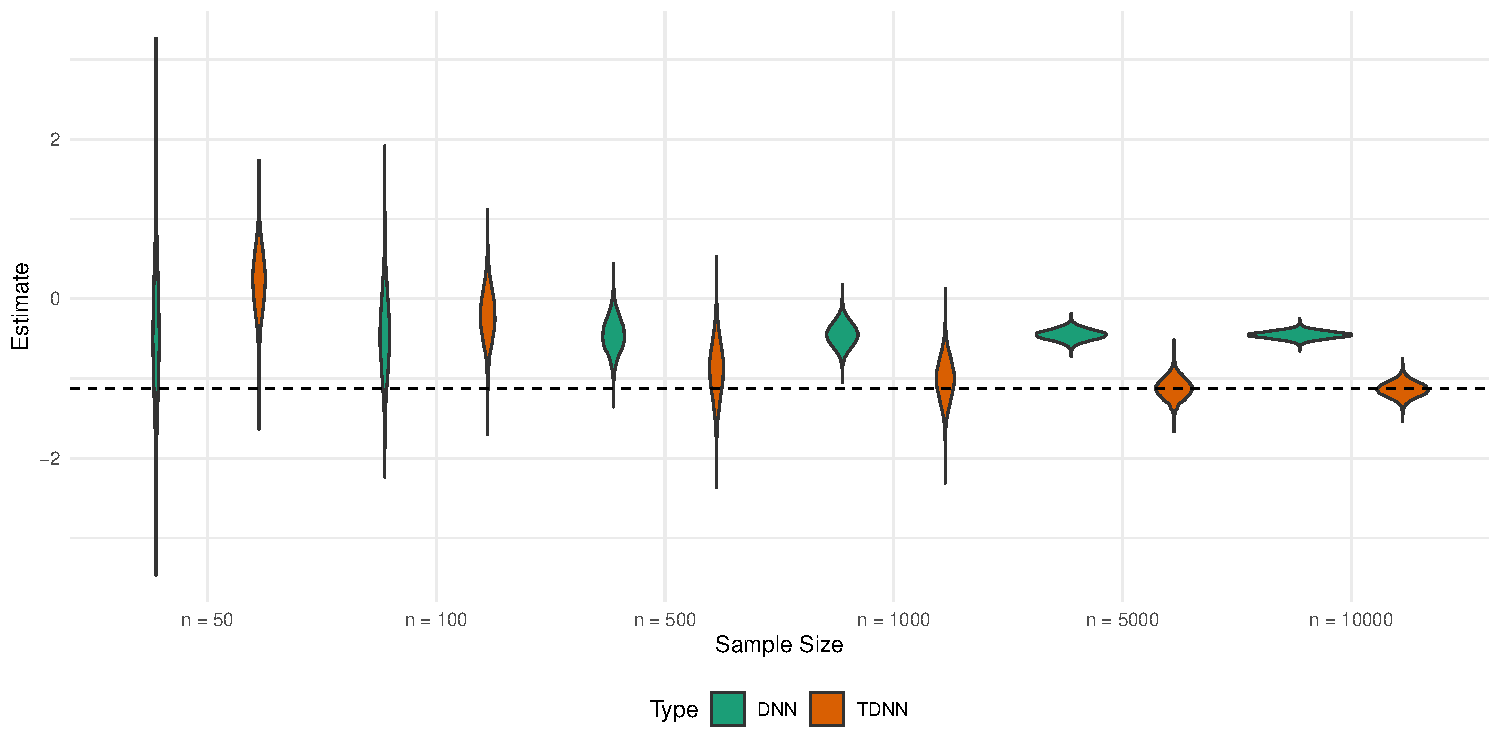
\includegraphics[width = \textwidth]{../Code/Simulations/Graphics/TDNN_DNN.pdf}
	\caption{Comparison of the DNN ($s = 20$) and TDNN ($s_1 = 20, s_2 = 50$) Estimators for different sample sizes.
		The dashed line indicates the value of the unknown regression function at the point of interest.
		Simulation Setup replicates Setting 1 from \citet{demirkaya_optimal_2024} for 10000 Monte Carlo Replications.}
	\label{fig:TDNN_bias_cor}
\end{figure}
As can be seen in Figure~\ref{fig:TDNN_bias_cor}, a suitable choice of subsampling scales can effectively reduce the bias of the TDNN estimator compared to the DNN estimator.
This reinforces the idea that the TDNN estimator can be a useful tool in practice that has the potential to improve on well-established nearest neighbor methods.

\newpage
As a second, potentially more illustrative example, we consider the estimation of a function of two arguments.
Specifically, we consider the function $\mu(x) = 5 \cdot \left(\cos(x_1) + \cos(x_2)\right)$ on $[0,1]^2$ with heteroskedastic error terms whose variance is determined by $\sigma_{\varepsilon}^2(x) = \frac{1}{16}\left(x_1^2 + x_2^2\right)^2$.
The resulting surface is shown in Figure~\ref{fig:reg_surface}.

\begin{figure}[H]
	\centering
	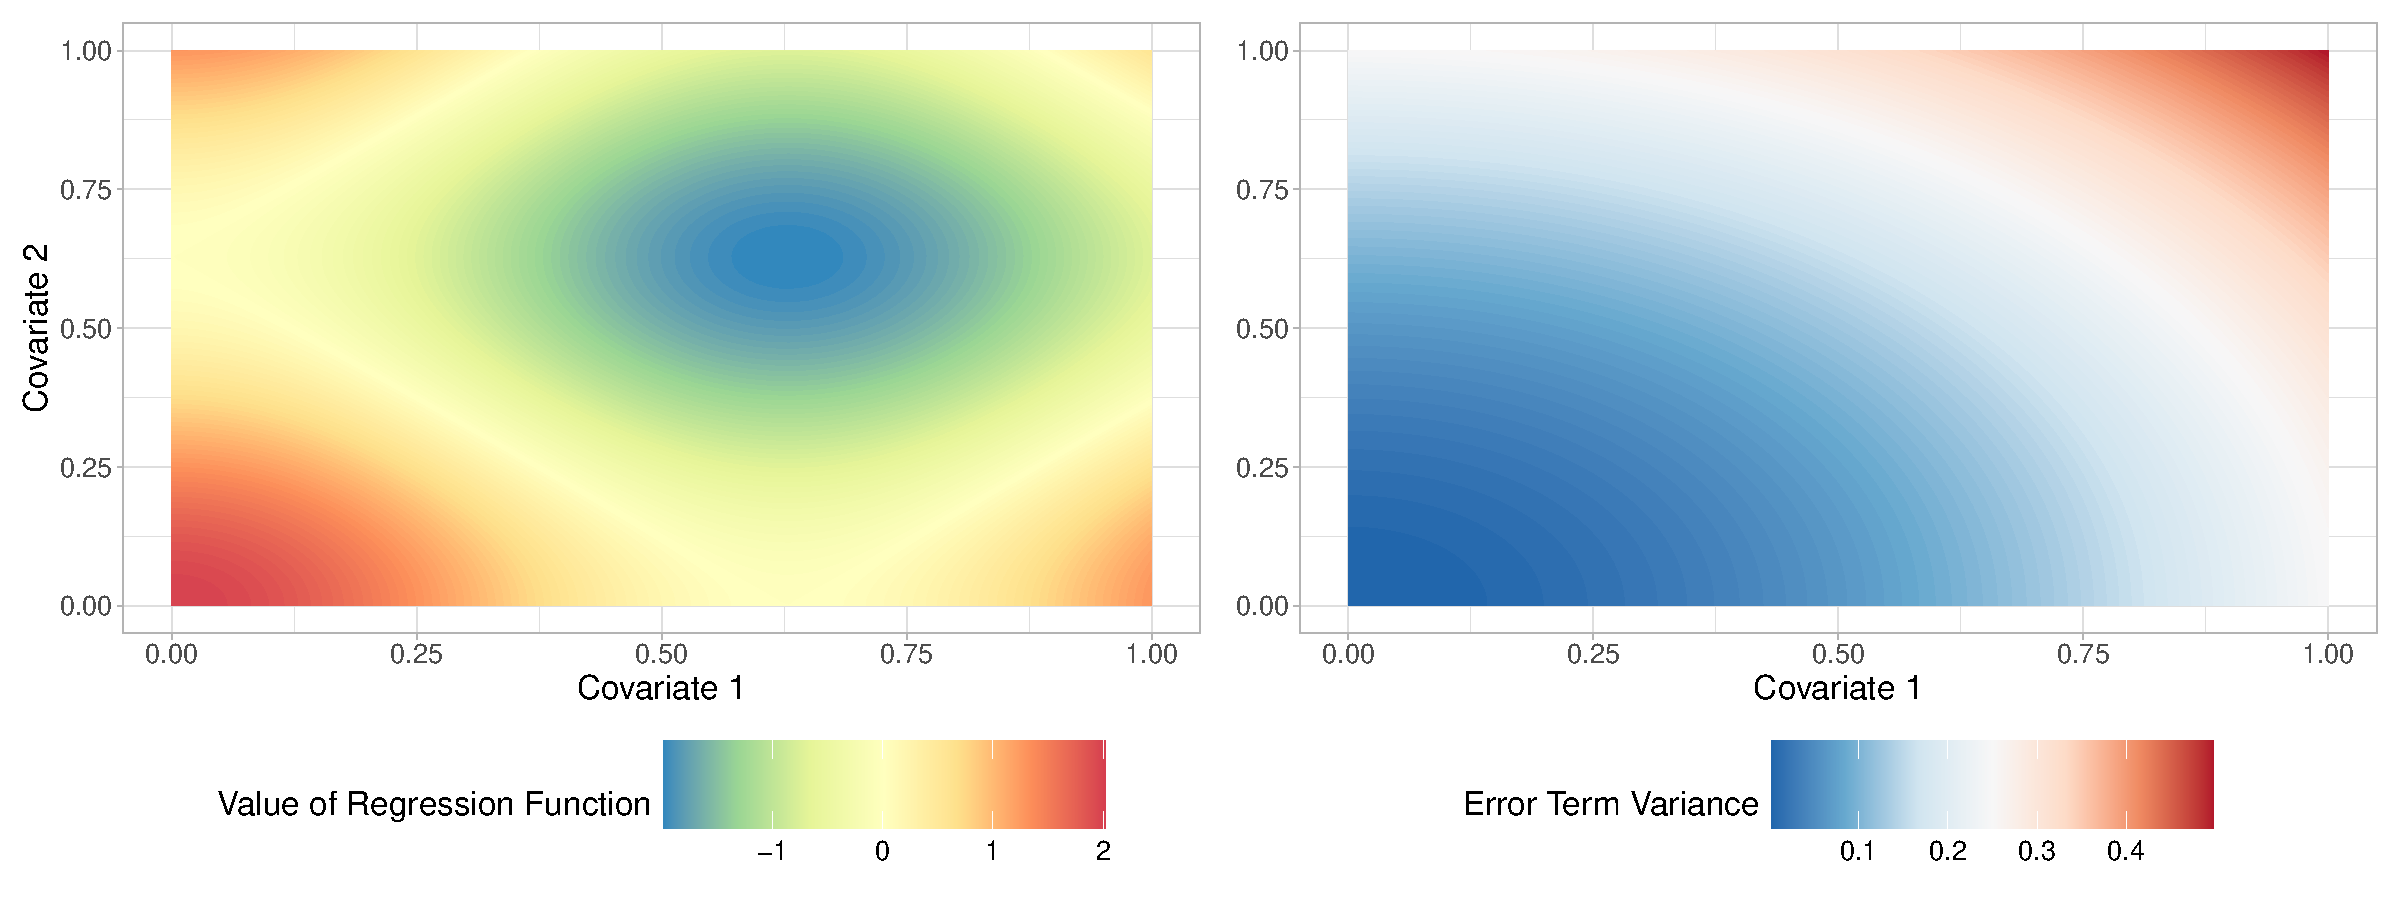
\includegraphics[width = \textwidth]{../Graphics/Reg_Exmp1.pdf}
	\caption{Value of the Regression Function (left) and Variance of the Error Term (right)}
	\label{fig:reg_surface}
\end{figure}
To analyze the behavior of the estimator in this setting, we run a number of Monte Carlo simulations each consisting of 10000 simulation runs.
While the theoretical analysis was of purely asymptotic nature, these simulation results can provide a modicum of guidance when it comes to choices such as the kernel orders employed in the estimation procedure.
Each run consists of 10000 observations that are uniformly distributed on ${[0,1]}^2$, and we find the following concerning the estimators bias and variance given different kernel orders $s_1$ and $s_2$.
\begin{figure}[H]
	\centering
	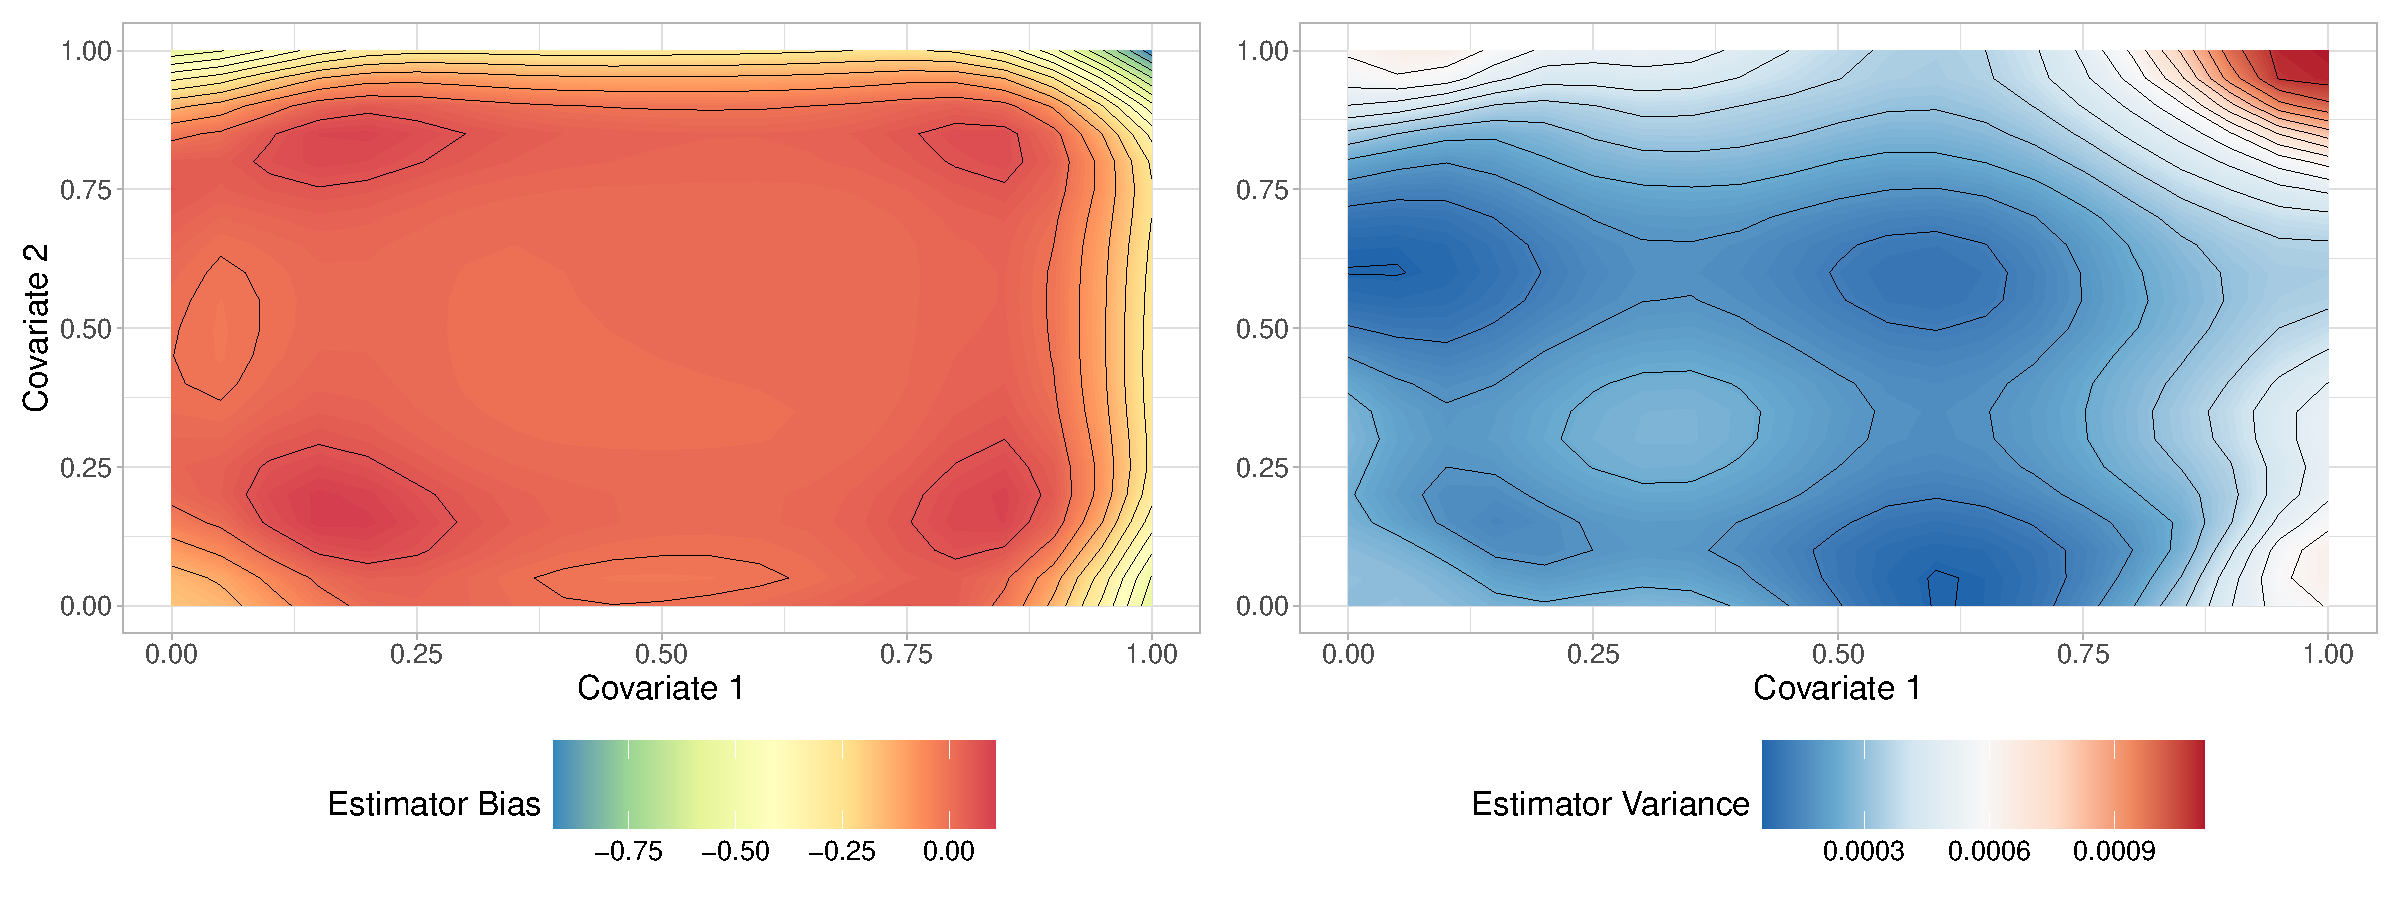
\includegraphics[width = \textwidth]{../Code/Simulations/Graphics/Reg_Exp1/TDNN/Plot_TDNN_n10000s_10_25.RDS.pdf}
	\caption{Approximate Bias (left) and Variance (right) of the TDNN Estimator with $s_1 = 10$ and $s_2 = 25$}
	\label{fig:est_bias_var_2}
\end{figure}
\begin{figure}[H]
	\centering
	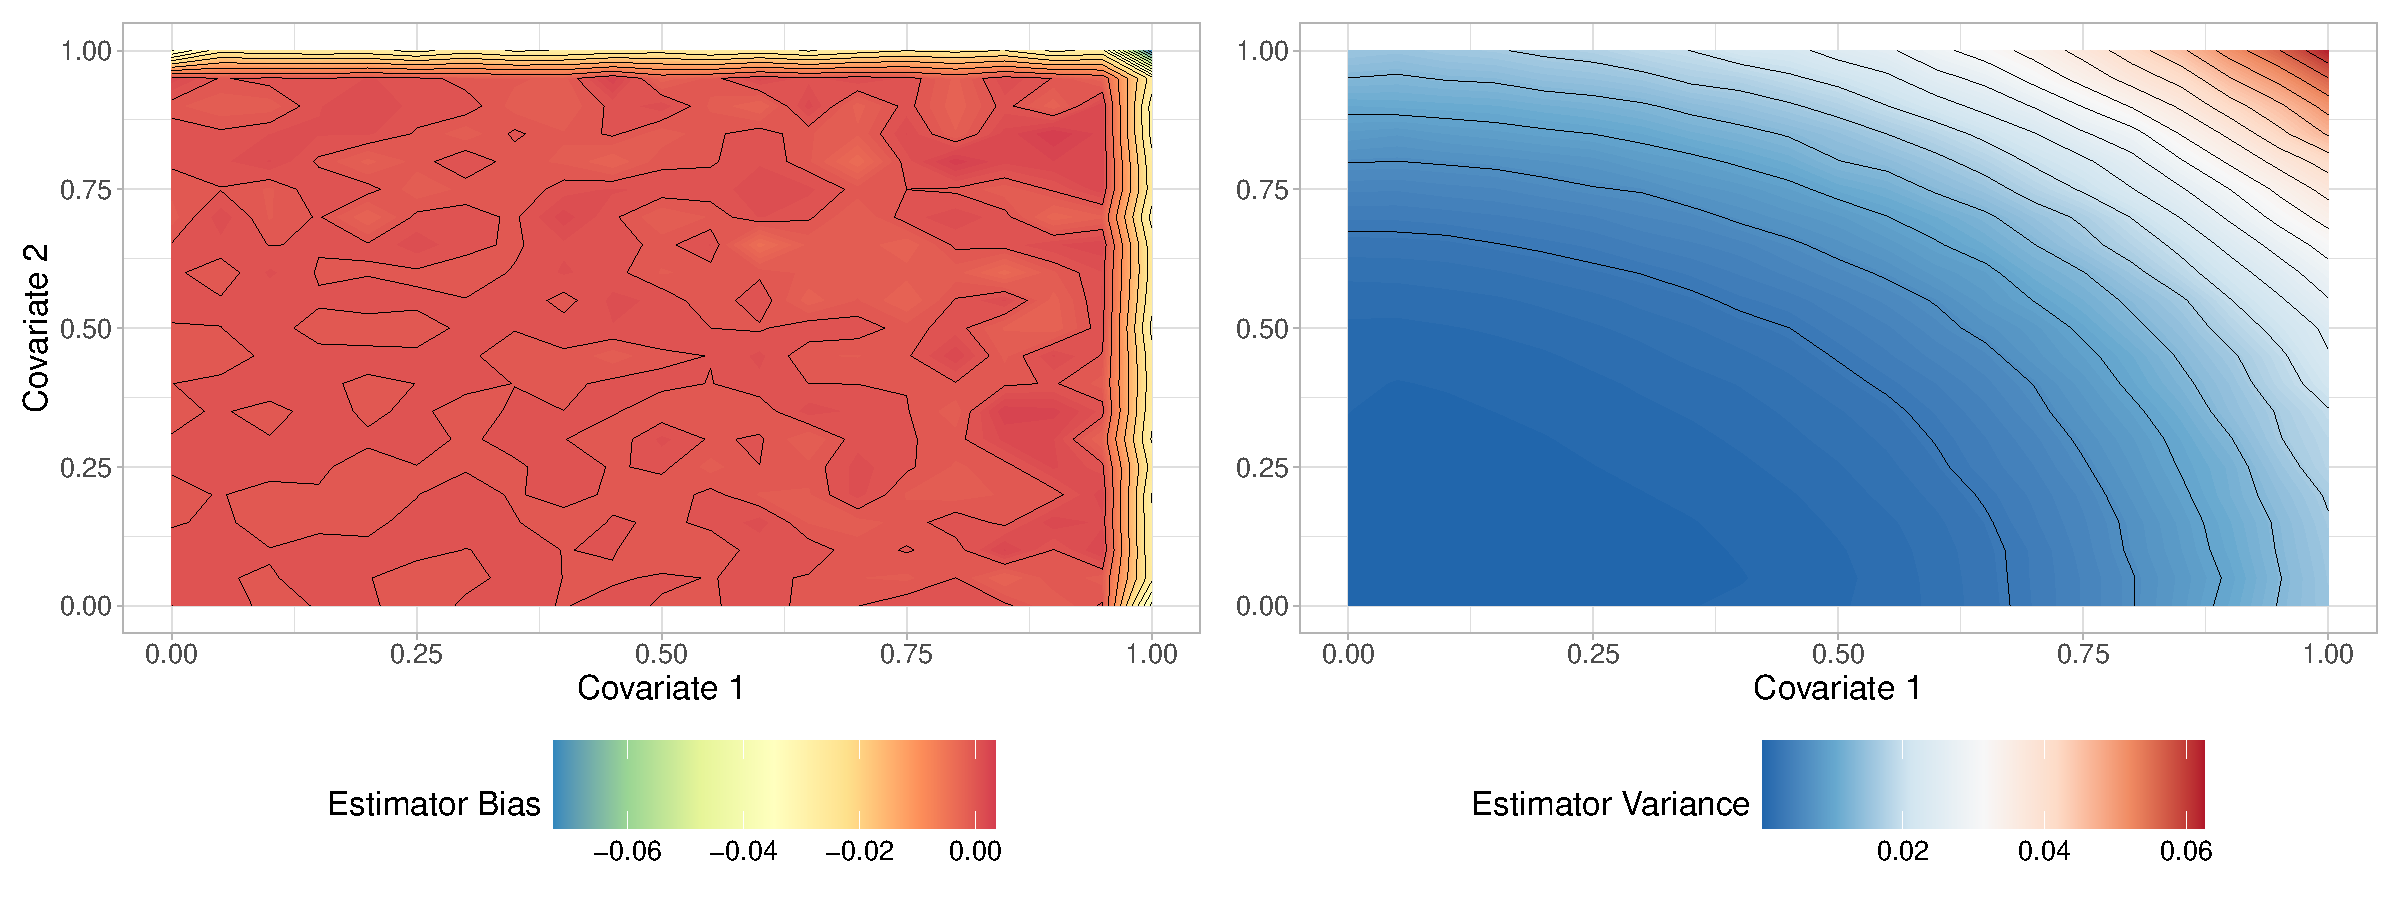
\includegraphics[width = \textwidth]{../Code/Simulations/Graphics/Reg_Exp1/TDNN/Plot_TDNN_n10000s_1000_2500.RDS.pdf}
	\caption{Approximate Bias (left) and Variance (right) of the TDNN Estimator with $s_1 = 1000$ and $s_2 = 2500$}
	\label{fig:est_bias_var}
\end{figure}


\subsection{CATE-Estimation}
\hrule

\begin{figure}[H]
	\centering
	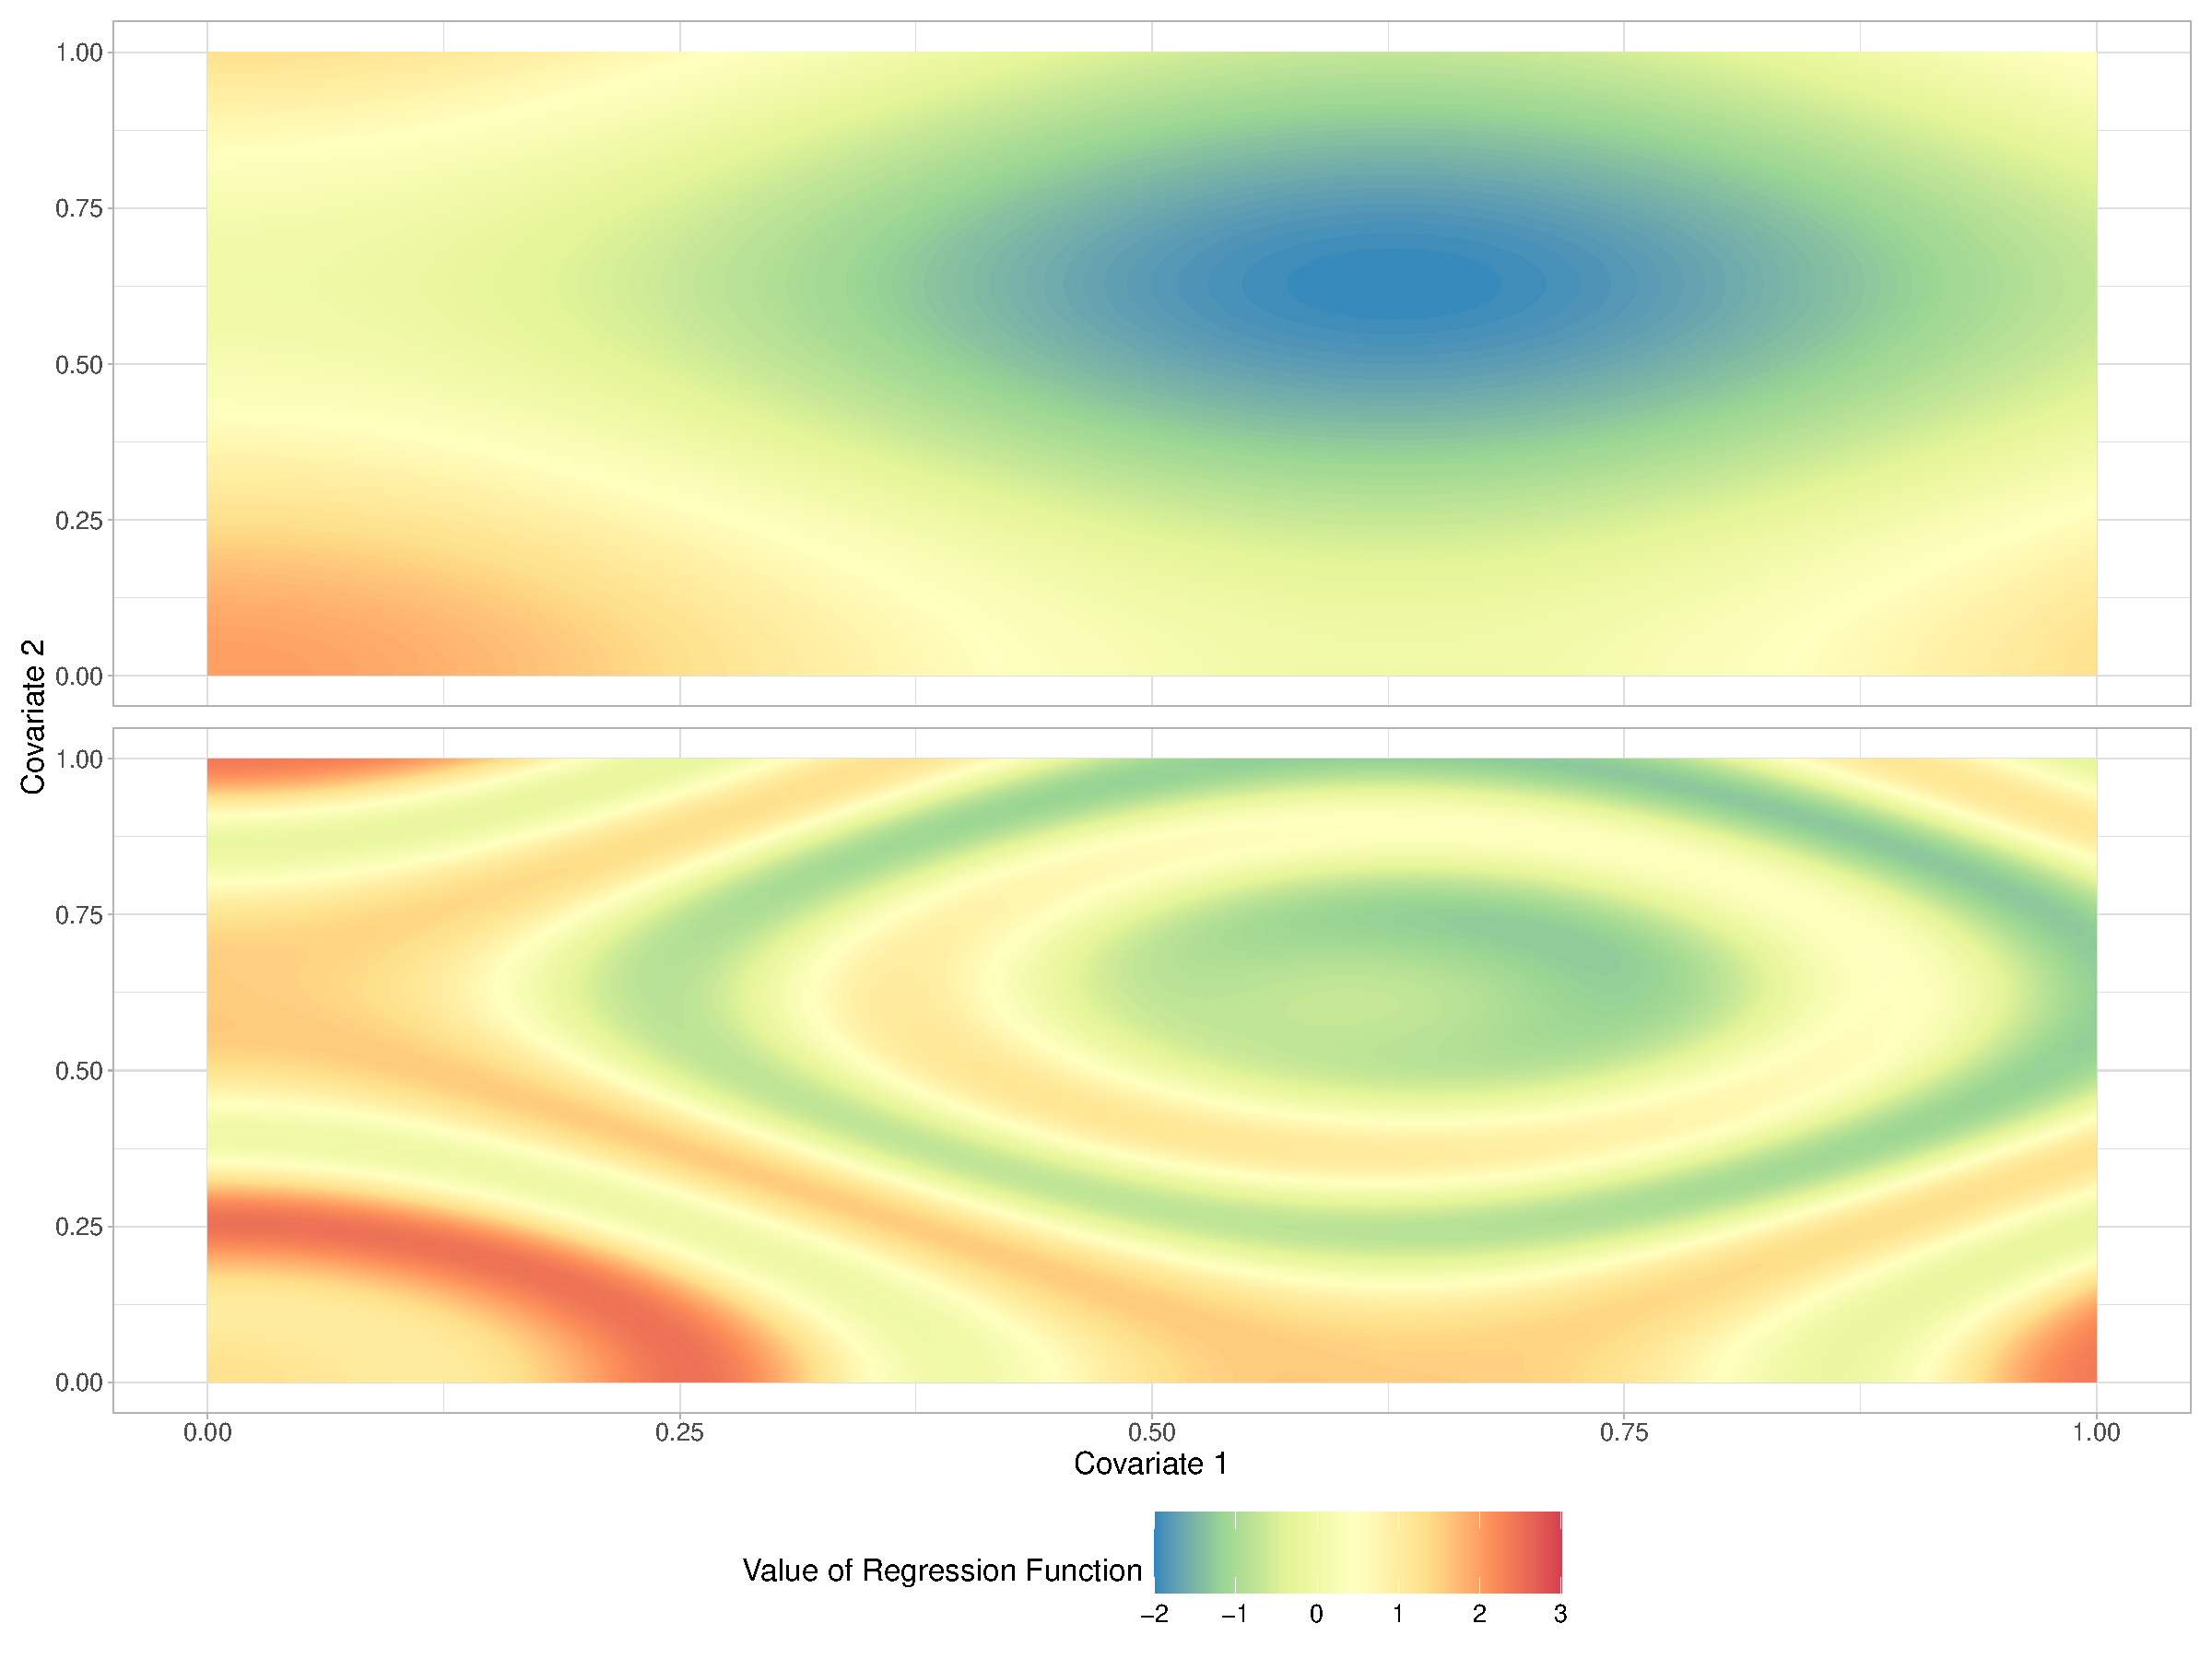
\includegraphics[width = \textwidth]{../Graphics/CATE_Exmp1.pdf}
	\caption{Value of the Regression Functions $\mu_0$ (upper) and $\mu_1$ (lower).	Error term structure remains unchanged.}
	\label{fig:CATE_surfaces}
\end{figure}

{\color{red} LOREM IPSUM}
\section{Application}\label{sec:application}
\hrule

I apply the method presented in this paper to the estimation of CATE in the well-studied \textit{National Job Training Partnership Act} (JTPA) Study.
Notable papers that have studied the same data set and might serve as useful points of reference include \citet{bloom_benefits_1997}, \citet{heckman_matching_1997}, \citet{abadie_instrumental_2002}, and \citet{kitagawa_who_2018}.
For the analysis presented in the following, I combined data provided by Josh Angrist in his data archive (\citet{abadie_replication_2008}) with data from the original data set provided by the W.E. Upjohn Institute for Employment Research to obtain the type of covariates to suitably illustrate the estimators performance in a real-world setting.
For this purpose, specifically to mimic a non-experimental setting, I restrict the data set to the individuals chosen to be eligible for treatment at random.
In essence, this takes the perspective of a decision maker that wants to evaluate the intent-to-treat CATE given observational data, a common scenario to determine eligibility criteria for policy measures.

{\color{red} LOREM IPSUM}
\section{Conclusion}\label{sec:conclusion}
\hrule
{\color{red} LOREM IPSUM}

\newpage
\printbibliography

\newpage
\appendix

\newpage
\section{Preparatory Definitions and Lemmas}
\hrule

\subsection{Definitions and Results on U-Statistics}
\hrule

Recall the definitions of Section \ref{sec:TDNN}.
First, for the DNN estimator and any $1 \leq c \leq s$, define
\begin{equation}\label{eq:xi_s_c}
	\xi_{s}^{c}\left(x\right)
	= \Var_{1:c}\left(\psi_{s}^{c}(x; Z_{1}, \dotsc, Z_{c})\right)
\end{equation}
where $Z_{c+1}^{\prime}, \ldots, Z_n^{\prime}$ are i.i.d.\ from $P$ and independent of $Z_1, \ldots, Z_n$ and thus
$\xi_{s}^{s}\left(x\right) = \Var\left(h_s\left(x; Z_1, \ldots, Z_s\right)\right)$.
% Then, I have the following result from the original paper.
Similarly, for the TDNN estimator and any $1 \leq c \leq s_2$, let
\begin{equation}\label{eq:zeta_s1s2_c}
	\zeta_{s_1, s_2}^{c}\left(x\right)
	= \Var_{1:c}\left(\psi_{s_1, s_2}^{c}(x; Z_{1}, \dotsc, Z_{c})\right)
\end{equation}
with an analogous definition of $Z^{\prime}$.
Standard results for U-statistics (see, for example, \citet{lee_u-statistics_2019}) give us a number of useful results.
First, an immediate result on the expectations of the Hoeffding-projection kernels.
\begin{align}\label{eq:H_k_expectation}
	\forall c = 1,2,\dotsc, j-1: \quad & \E_{D}\left[h_{s_1, s_2}^{(j)}\left(x; D\right) \, | \, Z_1 = \mathbf{z}_1, \dotsc, Z_c = \mathbf{z}_c\right] = 0
	\quad \text{and} \quad
	\E_{D}\left[h_{s_1, s_2}^{(j)}\left(x; D\right)\right] = 0
\end{align}
Second, I obtain a useful variance decomposition in terms of the Hoeffding-projection variances.
\begin{align}\label{eq:Var_decomp}
	\Var_{D}\left(\hat{\mu}_{s_1, s_2}\left(x; D\right)\right)
	 & = \sum_{j = 1}^{s_2} \binom{s_2}{j}^2 \Var_{D}\left(H_{s_1, s_2}^{j}\left(x; D\right)\right) \\
	%
	\Var_{D}\left(H_{s_1, s_2}^{j}\left(x; D\right)\right)
	 & = \binom{n}{j}^{-1} \Var_{D}\left(h_{s_1, s_2}^{(j)}\left(x; D\right)\right)
	=: \binom{n}{j}^{-1} V_{s_1, s_2}^{j}\left(x\right)
\end{align}
Third, the following equivalent expression for the kernel variance.
\begin{equation}\label{eq:k_var}
	\zeta_{s_1, s_2}^{s_2}\left(x\right)
	= \Var_{D}\left(h_{s_1, s_2}\left(x; D\right)\right)
	= \sum_{j = 1}^{s_2} \binom{s_2}{j}V_{s_1, s_2}^{j}
\end{equation}

\newpage
\section{Preparatory Lemmas}
\hrule

\subsection{Properties of the $\kappa$ Function}
\hrule

\begin{lem}[\citet{demirkaya_optimal_2024} - Lemma 12]\label{lem:dem12}\mbox{}\\*
	Let $D = \{Z_1, \dotsc, Z_s\}$ an i.i.d.\ sample drawn from $P$.
	The indicator functions $\kappa\left(x; Z_{i}, D\right)$ satisfy the following properties.
	\begin{enumerate}
		\item For any $i \neq j$, we have $\kappa\left(x; Z_{i}, D\right) \kappa\left(x;
			      Z_{j}, D\right)=0$ with probability one;
		\item $\sum_{i=1}^{s} \kappa\left(x; Z_{i}, D\right)=1$;
		\item $\forall i \in [s]: \quad \E_{1:s}\left[\kappa\left(x; Z_{i}, D\right)\right]=s^{-1}$
		\item $\E_{2: s}\left[\kappa\left(x; Z_1, D\right)\right]
			      = \left\{1-\varphi\left(B\left(x,\left\|X_1-x\right\|\right)\right)\right\}^{s-1}$
	\end{enumerate}
	Here $\E_{i: s}$ denotes the expectation with respect to $\left\{Z_{i}, Z_{i+1}, \dotsc, Z_s\right\}$.
	Furthermore, $\varphi$ denotes the probability measure on $\mathbb{R}^{d}$ induced by the random vector $X$.
\end{lem}

\hrule

\begin{lem}[\citet{demirkaya_optimal_2024} - Lemma 13]\label{lem:dem13}\mbox{}\\*
	For any $L^1$ function $f$ that is continuous at $x$, it holds that
	\begin{equation}
		\lim _{s \rightarrow \infty} \E_{1}\left[f\left(X_1\right) s \E_{2:s}\left[\kappa(x; Z_1, D)\right]\right]
		= f(x).
	\end{equation}
\end{lem}

\hrule

As an additional tool, we will make use of the following analogous results concerning products of two kernel functions with nonzero expectation.
These results will then be used to construct an analogon of Lemma \ref{lem:dem13} for the corresponding cases.
This will serve very similar purposes in the analysis of (conditional) covariance terms as the previous results serve for (conditional) expectations.
\vspace{0.5cm}
\hrule

\begin{lem}[]\label{lem:expec_kernel_prod}\mbox{}\\*
    Fix sample size $n$, subsampling scale $s$, and $c$ such that $0 < c \leq s \leq n$.
	Let $D = \left\{Z_1, Z_2, \dotsc, Z_c, Z_{c+1}, \dotsc Z_s \right\}$ be an i.i.d.\ data set drawn from $P$ as described in Setup~\ref{asm:npr_dgp}.
	Let $D^{\prime} = \left\{Z_1, Z_2, \dotsc, Z_c, Z_{c+1}^{\prime}, \dotsc Z_s^{\prime} \right\}$ be a second data set that shares the first $c$ observations with $D$.
	The remaining $s - c$ observations of $D^{\prime}$, i.e.\ $\left\{Z_{c+1}^{\prime}, \dotsc Z_s^{\prime} \right\}$, are i.i.d.\ draws from $P$ that are independent of $D$.

    Then the following three statements hold.
    \begin{equation}
        \forall i \in [c]: \quad
        \E_{D, D^{\prime}}\left[\kappa\left(x; Z_{i}, D\right)\kappa\left(x; Z_{i}, D^{\prime}\right)\right]
        = (2s - c)^{-1} = \omega(e^{-s})
    \end{equation}
    \begin{equation}
        \begin{aligned}
            \forall i \in [c] \; \forall j \in \{c+1, \dotsc, s\}: \quad
            \E_{D, D^{\prime}}\left[\kappa\left(x; Z_{i}, D\right)\kappa\left(x; Z_{j}^{\prime}, D^{\prime}\right)\right]
            & = \frac{1}{(2s - c)(2s-c-1)}\sum_{i = 0}^{s - c - 1}\binom{s - c - 1}{i}\binom{2s - c - 2}{i}^{-1} \\
            & = \omega(e^{-s})
        \end{aligned}
    \end{equation}
    \begin{equation}
        \begin{aligned}
            \forall i,j \in \{c+1, \dotsc, s\}: \quad
            \E_{D, D^{\prime}}\left[\kappa\left(x; Z_{i}, D\right)\kappa\left(x; Z_{j}^{\prime}, D^{\prime}\right)\right]
            & = \frac{2}{(2s-c)(2s-c-1)}\sum_{i = 0}^{s-c-1} \binom{s - c - 1}{i}\binom{2s - c - 1}{s-1+i}^{-1}\\
            %
            & = \omega(e^{-s})
        \end{aligned}
    \end{equation}
\end{lem}

\begin{proof}[Proof of Lemma \ref{lem:expec_kernel_prod}]\mbox{}\\*
    Without loss of generality, we will consider the cases of $i = 1$ and $j = c + 1$ for the first two equations.
    \begin{equation}
        \begin{aligned}
            \E_{D, D^{\prime}}\left[\kappa\left(x; Z_{1}, D\right)\kappa\left(x; Z_{1}, D^{\prime}\right)\right]
            & = \E_{D, D^{\prime}}\left[\kappa\left(x; Z_{1}, D_{1:c}\right)\kappa\left(x; Z_{1}, D_{(c+1):s}\right)\kappa\left(x; Z_{1}, D^{\prime}_{(c+1):s}\right)\right]\\
            %
            & = \E\left[\kappa\left(x; Z_{1}, D_{[2s - c]}\right)\right]
            = (2s - c)^{-1}
        \end{aligned}
    \end{equation}
    Considering the second case, we find the following.
    \begin{equation}
        \begin{aligned}
            & \E_{D, D^{\prime}}\left[\kappa\left(x; Z_{1}, D\right)\kappa\left(x; Z_{c+1}^{\prime}, D^{\prime}\right)\right]
            = \frac{1}{(2s - c)!} \sum_{i = 0}^{s - c - 1}\binom{s - c - 1}{i} i! \left((s - 1) + (s - c - 1 - i)\right)! \\
            %
            & \quad = \frac{1}{(2s - c)!}\sum_{i = 0}^{s - c - 1}\binom{s - c - 1}{i} i! \left(2s - c - 2 - i\right)! 
            = \frac{(2s - c - 2)!}{(2s - c)!}\sum_{i = 0}^{s - c - 1}\binom{s - c - 1}{i}\binom{2s - c - 2}{i}^{-1}
        \end{aligned}
    \end{equation}
    While unintuitive at first, the terms in this expression have intuitive meaning when we consider this as a combinatoric problem.
    Consider lining up the observations in order of their distance to the point of interest and counting the cases for which the expression in the expectation is equal to one.
    First, there are $(2s-c)!$ possible orderings of the observations with probability one, leading to the denominator.
    Next, notice that only those orderings where $\|X_{c+1}^{\prime} - x\| \leq \|X_{1}-x\|$ and $\|X_{1} - x\| \leq \|X_{i} - x\|$ for any $i = 2, \dotsc, c$ can possibly lead to a non-zero realization of the kernel term.
    Furthermore, out of the $(s-c-1)$ observations in $D^{\prime}_{(c+2):s}$, it is possible for $i = 0, \dotsc, s-c-1$ observations to lie at a distance to the point of interest that is smaller than $\|X_{1}-x\|$ but larger than $\|X_{c+1}^{\prime} - x\|$ in any permutation.
    The sum adjusts for those possible configurations.
    Next, we can make the following observation concerning the expression we just derived.
    \begin{equation}
        \begin{aligned}
            \E_{D, D^{\prime}}\left[\kappa\left(x; Z_{1}, D\right)\kappa\left(x; Z_{c+1}^{\prime}, D^{\prime}\right)\right]
            & \geq \frac{1}{(2s - c)(2s-c-1)}\sum_{i = 0}^{s - c - 1}\frac{(s - c - i)^{i}}{i!}\frac{i!}{(2s-c-2)^{i}} \\
            %
            & = \frac{1}{(2s - c)(2s-c-1)}\left(1 + \sum_{i = 0}^{s - c - 1}\left(\frac{s - c - i}{2s-c-2}\right)^{i}\right)\\
            %
            & \geq \frac{1}{(2s - c)^{2}}
        \end{aligned}
    \end{equation}
    We can now observe the following using the small Omega Bachmann-Landau notation.
    \begin{equation}
        \lim_{s \rightarrow \infty} \frac{(2s-c)^{-2}}{e^{-s}} = \infty
        \quad \implies \quad
        \E_{D, D^{\prime}}\left[\kappa\left(x; Z_{1}, D\right)\kappa\left(x; Z_{c+1}^{\prime}, D^{\prime}\right)\right]
        = \omega(e^{-x})
    \end{equation}
    
    Considering the third case, without loss of generality, we consider the case of $i = j = c+1$.
    We find the following.
    \begin{equation}
        \begin{aligned}
            & \E_{D, D^{\prime}}\left[\kappa\left(x; Z_{c+1}, D\right)\kappa\left(x; Z_{c+1}^{\prime}, D^{\prime}\right)\right]\\
            %
            & \quad  = \E_{D, D^{\prime}}\left[
                \kappa\left(x; Z_{c+1}, D_{1:c}\right)\kappa\left(x; Z_{c+1}^{\prime}, D_{1:c}\right)
                \kappa\left(x; Z_{c+1}, D_{(c+1):s}\right)\kappa\left(x; Z_{c+1}^{\prime}, D_{(c+1):s}^{\prime}\right)
            \right]\\
            %
            & \quad = \frac{2}{(2s - c)!} \sum_{i = 0}^{s-c-1} \binom{s - c - 1}{i}(s - 1 + i)!(s-c-1-i)! \\
            %
            & \quad = \frac{2(2s - c - 2)!}{(2s-c)!} \sum_{i = 0}^{s-c-1} \binom{s - c - 1}{i}\binom{2s - c - 2}{s-1+i}^{-1} \\
            %
            & \quad = \frac{2}{(2s-c)(2s-c-1)}\sum_{i = 0}^{s-c-1} \binom{s - c - 1}{i}\binom{2s - c - 2}{s-1+i}^{-1}
        \end{aligned}
    \end{equation}
    The third case follows from a similar combinatorial logic as the second.
    We consider without loss of generality the case that $\|X_{c+1}^{\prime} - x\| \leq \|X_{c+1}-x\|$ and adjust for this fact by multiplying the whole expression by two.
    Notice now that any number $i = 0, \dotsc, s-c-1$ of observations in $D^{\prime}_{(c+2):s}$ can be farther away from $x$ than $X_{c+1}$ or at a distance that is between $\|X_{c+1}^{\prime} - x\|$ and $\|X_{c+1}-x\|$.
    The summation adjusts for all possible permutations that fulfill this criterion.
    Furthermore, we can make the following observation.
    \begin{equation}
        \begin{aligned}
            & \E_{D, D^{\prime}}\left[\kappa\left(x; Z_{c+1}, D\right)\kappa\left(x; Z_{c+1}^{\prime}, D^{\prime}\right)\right]
            \geq \frac{1}{(2s-c)^{2}}\sum_{i = 0}^{s-c-1} \binom{s - c - 1}{i}\binom{2s - c - 2}{s-1+i}^{-1} \\
            %
            & \quad = \frac{1}{(2s-c)^{2}}\sum_{i = 0}^{s-c-1} \left(\frac{(s-c-1)!}{i!(s-c-1-i)!} \cdot \frac{(s-1+i)!(s-c-1-i)!}{(2s-c-2)!}\right)\\
            %
            & \quad = \frac{1}{(2s-c)^{2}} \cdot \frac{(s-c-1)!}{(2s-c-2)!}\sum_{i = 0}^{s-c-1} \frac{(s-1+i)!}{i!}\\
            %
            & \quad = \frac{1}{(2s-c)^{2}} \cdot \frac{(s-c-1)!}{(2s-c-2)!}\left(\frac{(2s-c-2)!}{(s-c-1)!} + \sum_{i = 0}^{s-c-2} \frac{(s-1+i)!}{i!}\right)\\
            %
            & \quad \geq \frac{1}{(2s-c)^{2}}
        \end{aligned}
    \end{equation}
        We can now observe the following using the small Omega Bachmann-Landau notation.
    \begin{equation}
        \lim_{s \rightarrow \infty} \frac{(2s-c)^{-2}}{e^{-s}} = \infty
        \quad \implies \quad
        \E_{D, D^{\prime}}\left[\kappa\left(x; Z_{c+1}, D\right)\kappa\left(x; Z_{c+1}^{\prime}, D^{\prime}\right)\right]
        = \omega(e^{-x})
    \end{equation}
\end{proof}

\hrule

\newpage
\begin{lem}[]\label{lem:cond_expec_kernel_prod}\mbox{}\\*
    Fix sample size $n$, subsampling scale $s$, and $c$ such that $0 < c \leq s \leq n$.
	Let $D = \left\{Z_1, Z_2, \dotsc, Z_c, Z_{c+1}, \dotsc Z_s \right\}$ be an i.i.d.\ data set drawn from $P$ as described in Setup~\ref{asm:npr_dgp}.
	Let $D^{\prime} = \left\{Z_1, Z_2, \dotsc, Z_c, Z_{c+1}^{\prime}, \dotsc Z_s^{\prime} \right\}$ be a second data set that shares the first $c$ observations with $D$.
	The remaining $s - c$ observations of $D^{\prime}$, i.e.\ $\left\{Z_{c+1}^{\prime}, \dotsc Z_s^{\prime} \right\}$, are i.i.d.\ draws from $P$ that are independent of $D$.

    Then, the following statements hold.
    \begin{equation}
        \begin{aligned}
            & \forall i \in [c]: \quad
            \E\left[\kappa\left(x; Z_{i}, D\right)\kappa\left(x; Z_{i}, D^{\prime}\right) \; \middle| \; X_i\right]
            = \left\{1-\varphi\left(B\left(x,\left\|X_{i}-x\right\|\right)\right)\right\}^{2s-c-1} 
        \end{aligned}
    \end{equation}
    \begin{equation}
        \begin{aligned}
            & \forall i \in [c] \; \forall j \in \{c+1, \dotsc, s\}: \quad
            \E\left[\kappa\left(x; Z_{i}, D\right)\kappa\left(x; Z_{j}^{\prime}, D^{\prime}\right) \; \middle| \; X_i, X_{j}^{\prime}\right]\\
            %
            & \quad = \1\left(\|X_{j}^{\prime} - x\| \leq \|X_{i} - x\|\right)
            \cdot \left\{1-\varphi\left(B\left(x,\left\|X_{i}-x\right\|\right)\right)\right\}^{s-1} 
            \cdot \left\{1-\varphi\left(B\left(x,\left\|X_{j}^{\prime}-x\right\|\right)\right)\right\}^{s-c-1}
        \end{aligned}
    \end{equation}
    \begin{equation}
        \begin{aligned}
            & \forall i,j \in \{c+1, \dotsc, s\}: \quad
            \E\left[\kappa\left(x; Z_{i}, D\right)\kappa\left(x; Z_{j}^{\prime}, D^{\prime}\right) \; \middle| \; X_{i}, X_{j}^{\prime}\right] \\ 
            %
            & \quad = \left\{1-\varphi\left(B\left(x, \min\left(\left\|X_{i} - x\right\|, \left\|X_{j}^{\prime}-x\right\|\right)\right)\right)\right\}^{s-c-1}
            \cdot \left\{1-\varphi\left(B\left(x,\max\left(\left\|X_{i} - x\right\|, \left\|X_{j}^{\prime}-x\right\|\right)\right)\right)\right\}^{s-1}
        \end{aligned}
    \end{equation}
\end{lem}

\begin{proof}[Proof of Lemma \ref{lem:cond_expec_kernel_prod}]\mbox{}\\*
    Without loss of generality, we will consider the cases of $i = 1$ for the first equation.
    \begin{equation}
        \begin{aligned}
            & \E\left[\kappa\left(x; Z_{1}, D\right)\kappa\left(x; Z_{1}, D^{\prime}\right) \; \middle| \; X_1\right]
            = \E\left[\kappa\left(x; Z_{1}, D_{[c]}\right)
            \kappa\left(x; Z_{1}, D_{(c+1):s}\right)
            \kappa\left(x; Z_{1}, D^{\prime}_{(c+1):s}\right) 
            \; \middle| \; X_1\right] \\
            %
            & \quad = \E\left[\kappa\left(x; Z_{1}, D_{[c]}\right)\; \middle| \; X_1\right]
            \cdot \E\left[\kappa\left(x; Z_{1}, D_{(c+1):s}\right)\; \middle| \; X_1\right]
            \cdot \E\left[\kappa\left(x; Z_{1}, D_{(c+1):s}^{\prime}\right)\; \middle| \; X_1\right]\\
            %
            & \quad = \left\{1-\varphi\left(B\left(x,\left\|X_{i}-x\right\|\right)\right)\right\}^{c-1}
            \cdot \left\{1-\varphi\left(B\left(x,\left\|X_{i}-x\right\|\right)\right)\right\}^{s-c}
            \cdot \left\{1-\varphi\left(B\left(x,\left\|X_{i}-x\right\|\right)\right)\right\}^{s-c} \\
            %
            & \quad = \left\{1-\varphi\left(B\left(x,\left\|X_{i}-x\right\|\right)\right)\right\}^{2s-c-1}
        \end{aligned}
    \end{equation}
    Without loss of generality, we will consider the cases of $i = 1$ and $j = c + 1$ for the second equation.
    \begin{equation}
    \begin{aligned}
        & \E\left[\kappa\left(x; Z_{1}, D\right)\kappa\left(x; Z_{c+1}^{\prime}, D^{\prime}\right) \; \middle| \; X_1, X_{c+1}^{\prime}\right]\\
        %
        & = \E\left[
                \E\left[
                    \kappa\left(x; Z_{1}, D_{1:c}\right)
                    \kappa\left(x; Z_{1}, D_{(c+1):s}\right)
                    \kappa\left(x; Z_{c+1}^{\prime}, D_{1:c}\right) 
                    \kappa\left(x; Z_{c+1}^{\prime}, D^{\prime}_{(c+1):s}\right) 
                \; \middle| \; X_1, \dotsc, X_{c}, X_{c+1}^{\prime}\right] 
            \; \middle| \; X_1, X_{c+1}^{\prime}\right] \\
		%
        & = \E\left[
                \E\left[
                    \kappa\left(x; Z_{1}, D_{(c+1):s}\right)
                    \cdot \kappa\left(x; Z_{c+1}^{\prime}, D^{\prime}_{(c+1):s}\right)
                \; \middle| \; X_1, \dotsc, X_{c}, X_{c+1}^{\prime}\right] 
                \cdot \kappa\left(x; Z_{1}, D_{1:c}\right)
                \cdot \kappa\left(x; Z_{c+1}^{\prime}, D_{1:c}\right)
            \; \middle| \; X_1, X_{c+1}^{\prime}\right] \\
        %
        & = \E\left[
                \E\left[
                    \kappa\left(x; Z_{1}, D_{(c+1):s}\right)
                    \cdot \kappa\left(x; Z_{c+1}^{\prime}, D^{\prime}_{(c+1):s}\right)
                \; \middle| \; X_1, X_{c+1}^{\prime}\right] 
                \cdot \kappa\left(x; Z_{1}, D_{1:c}\right)
                \cdot \kappa\left(x; Z_{c+1}^{\prime}, D_{1:c}\right)
            \; \middle| \; X_1, X_{c+1}^{\prime}\right] \\
        %
        & = \E\left[
                    \kappa\left(x; Z_{1}, D_{(c+1):s}\right)
                    \cdot \kappa\left(x; Z_{c+1}^{\prime}, D^{\prime}_{(c+1):s}\right)
            \; \middle| \; X_1, X_{c+1}^{\prime}\right] 
            \cdot \E\left[
                \kappa\left(x; Z_{1}, D_{1:c}\right)
                \cdot \kappa\left(x; Z_{c+1}^{\prime}, D_{1:c}\right)
            \; \middle| \; X_1, X_{c+1}^{\prime}\right] \\
        %
        & = \E\left[\kappa\left(x; Z_{1}, D_{(c+1):s}\right)\; \middle| \; X_1\right] 
            \cdot \E\left[\kappa\left(x; Z_{c+1}^{\prime}, D^{\prime}_{(c+1):s}\right)
            \; \middle| \; X_{c+1}^{\prime}\right] 
            \cdot \1\left(\|X_{c+1}^{\prime} - x\| \leq \|X_{1} - x\|\right)
            \cdot \E\left[
                \kappa\left(x; Z_{1}, D_{1:c}\right)
            \; \middle| \; X_1\right] \\
        %
        & = \1\left(\|X_{c+1}^{\prime} - x\| \leq \|X_{1} - x\|\right)
        \cdot \E\left[\kappa\left(x; Z_{1}, D\right)\; \middle| \; X_1\right] 
        \cdot \E\left[\kappa\left(x; Z_{c+1}^{\prime}, D^{\prime}_{(c+1):s}\right)
            \; \middle| \; X_{c+1}^{\prime}\right] \\
        %
        & = \1\left(\|X_{c+1}^{\prime} - x\| \leq \|X_{1} - x\|\right)
            \cdot \left\{1-\varphi\left(B\left(x,\left\|X_1-x\right\|\right)\right)\right\}^{s-1}
            \cdot \left\{1-\varphi\left(B\left(x,\left\|X_{c+1}^{\prime}-x\right\|\right)\right)\right\}^{s-c-1}
    \end{aligned}
    \end{equation}
    For the third case, without loss of generality, we consider the case of $i = j = c+1$.
    \begin{equation}
		\begin{aligned}
			& \E\left[
            \kappa\left(x; Z_{c+1}, D\right)
            \kappa\left(x; Z_{c+1}^{\prime}, D^{\prime}\right) \; \middle| \; X_{c+1}, X_{c+1}^{\prime}\right] \\
            % 
			& \quad = \E\left[
                \E\left[
                    \kappa\left(x; Z_{c+1}, D\right)
                    \kappa\left(x; Z_{c+1}^{\prime}, D^{\prime}\right) 
                \; \middle| \; X_{1}, \dotsc, X_{c}, X_{c+1}, X_{c+1}^{\prime}\right]
                \; \middle| \; X_{c+1}, X_{c+1}^{\prime} \right]\\
            % 
			& \quad = \E\left[
            \E\left[
                \kappa\left(x; Z_{c+1}, D_{1:(c+1)}\right)
                \kappa\left(x; Z_{c+1}^{\prime}, D^{\prime}_{1:(c+1)}\right) \right. \right. \\
                & \quad \quad \left. \left.
                \kappa\left(x; Z_{c+1}, D_{(c+1):s}\right)
                \kappa\left(x; Z_{c+1}^{\prime}, D^{\prime}_{(c+1):s}\right)
                \; \middle| \; X_{1}, \dotsc, X_{c}, X_{c+1}, X_{c+1}^{\prime}\right]
                \; \middle| \; X_{c+1}, X_{c+1}^{\prime} \right]\\
            % 
            & \quad = \E\left[
            \E\left[
                \kappa\left(x; Z_{c+1}, D_{1:(c+1)}\right)
                \kappa\left(x; Z_{c+1}^{\prime}, D^{\prime}_{1:(c+1)}\right) \; \middle| \; X_{1}, \dotsc, X_{c}, X_{c+1}, X_{c+1}^{\prime}\right] \right. \\
                & \quad \quad  \left.
                \kappa\left(x; Z_{c+1}, D_{(c+1):s}\right)
                \kappa\left(x; Z_{c+1}^{\prime}, D^{\prime}_{(c+1):s}\right)
                \; \middle| \; X_{c+1}, X_{c+1}^{\prime} \right]\\
            % 
			& \quad = \E\left[
                \kappa\left(x; Z_{c+1}, D_{1:(c+1)}\right)
                \kappa\left(x; Z_{c+1}^{\prime}, D^{\prime}_{1:(c+1)}\right)
                \; \middle| \; X_{c+1}, X_{c+1}^{\prime}\right] \\
                & \quad \quad  
                \cdot \E\left[\kappa\left(x; Z_{c+1}, D_{(c+1):s}\right)\; \middle| \; X_{c+1}\right]
                \cdot \E\left[\kappa\left(x; Z_{c+1}^{\prime}, D^{\prime}_{(c+1):s}\right)\; \middle| \; X_{c+1}^{\prime} \right]
		\end{aligned}
	\end{equation}
    Without loss of generality, consider the case that $\|X_{c+1} - x\| \leq \|X_{c+1}^{\prime} - x\|$.
    \begin{equation}
        \E\left[
            \kappa\left(x; Z_{c+1}, D_{1:(c+1)}\right)
            \kappa\left(x; Z_{c+1}^{\prime}, D^{\prime}_{1:(c+1)}\right)
            \; \middle| \; X_{c+1}, X_{c+1}^{\prime}\right] 
        = \E\left[
            \kappa\left(x; Z_{c+1}^{\prime}, D^{\prime}_{1:(c+1)}\right)
            \; \middle| \; X_{c+1}^{\prime}\right]
    \end{equation}
    Furthermore, observe the following.
    \begin{equation}
        \E\left[\kappa\left(x; Z_{c+1}^{\prime}, D^{\prime}_{1:(c+1)}\right) \; \middle| \; X_{c+1}^{\prime}\right]
        \cdot \E\left[\kappa\left(x; Z_{c+1}^{\prime}, D^{\prime}_{(c+1):s}\right)\; \middle| \; X_{c+1}^{\prime} \right]
        = \E\left[\kappa\left(x; Z_{c+1}^{\prime}, D^{\prime}\right)\; \middle| \; X_{c+1}^{\prime} \right]
    \end{equation}
    Thus, we can find the following.
    \begin{equation}
        \begin{aligned}
            & \E\left[\kappa\left(x; Z_{1}, D\right)\kappa\left(x; Z_{c+1}^{\prime}, D^{\prime}\right) \; \middle| \; X_1, X_{c+1}^{\prime}\right]\\
            & \quad = \1\left(\|X_{c+1}^{\prime} - x\| \leq \|X_{c+1} - x\|\right)
            \cdot \left\{1-\varphi\left(B\left(x,\left\|X_{c+1} - x\right\|\right)\right)\right\}^{s-1}
            \cdot \left\{1-\varphi\left(B\left(x,\left\|X_{c+1}^{\prime}-x\right\|\right)\right)\right\}^{s-c-2}\\
            & \quad \quad + \1\left(\|X_{c+1}^{\prime} - x\| > \|X_{c+1} - x\|\right)
            \cdot \left\{1-\varphi\left(B\left(x,\left\|X_{c+1} - x\right\|\right)\right)\right\}^{s-c-1}
            \cdot \left\{1-\varphi\left(B\left(x,\left\|X_{c+1}^{\prime}-x\right\|\right)\right)\right\}^{s-1}\\
            %
            & \quad = \left\{1-\varphi\left(B\left(x, \min\left(\left\|X_{c+1} - x\right\|, \left\|X_{c+1}^{\prime}-x\right\|\right)\right)\right)\right\}^{s-c-1}
            \cdot \left\{1-\varphi\left(B\left(x,\max\left(\left\|X_{c+1} - x\right\|, \left\|X_{c+1}^{\prime}-x\right\|\right)\right)\right)\right\}^{s-1}
        \end{aligned}
    \end{equation}
\end{proof}

\newpage

\begin{lem}[]\label{lem:kernel_prod_dirac_convergence}\mbox{}\\*
    Fix sample size $n$, subsampling scale $s$, and $c$ such that $0 < c \leq s \leq n$.
	Let $D = \left\{Z_1, Z_2, \dotsc, Z_c, Z_{c+1}, \dotsc Z_s \right\}$ be an i.i.d.\ data set drawn from $P$ as described in Setup~\ref{asm:npr_dgp}.
	Let $D^{\prime} = \left\{Z_1, Z_2, \dotsc, Z_c, Z_{c+1}^{\prime}, \dotsc Z_s^{\prime} \right\}$ be a second data set that shares the first $c$ observations with $D$.
	The remaining $s - c$ observations of $D^{\prime}$, i.e.\ $\left\{Z_{c+1}^{\prime}, \dotsc Z_s^{\prime} \right\}$, are i.i.d.\ draws from $P$ that are independent of $D$.

    For any $L^{2}(\mathcal{X})$ function $f$ that is continuous at $x$, it holds that
    \begin{equation}
        \lim_{s \rightarrow \infty} \underbrace{\E_{1}\left[f^{2}(X_{1}) (2s - c) 
            \E_{2:s}\left[\kappa\left(x; Z_{1}, D\right)\kappa\left(x; Z_{1}, D^{\prime}\right)\right]
        \right]}_{(A)}
        = f^{2}(x)
    \end{equation}
    \begin{equation}
        \lim_{s \rightarrow \infty} \underbrace{\E_{1, (c+1)^{\prime}}\left[
            f(X_{1}) f(X_{c+1}^{\prime})
            \cdot \frac{\E_{D, D^{\prime}}\left[\kappa\left(x; Z_{1}, D\right)\kappa\left(x; Z_{c+1}^{\prime}, D^{\prime}\right) \; \middle| \; Z_{1}, Z_{c+1}^{\prime}\right]}{\E_{D, D^{\prime}}\left[\kappa\left(x; Z_{1}, D\right)\kappa\left(x; Z_{c+1}^{\prime}, D^{\prime}\right)\right]}
        \right]}_{(B)}
        = f^{2}(x)
    \end{equation}
    \begin{equation}
        \lim_{s \rightarrow \infty} \underbrace{\E_{c+1}\left[
            f(X_{c+1}) f(X_{c+1}^{\prime})
            \cdot \frac{\E_{D, D^{\prime}}\left[\kappa\left(x; Z_{c+1}, D\right)\kappa\left(x; Z_{c+1}^{\prime}, D^{\prime}\right) \; \middle| \; Z_{c+1}, Z_{c+1}^{\prime}\right]}{\E_{D, D^{\prime}}\left[\kappa\left(x; Z_{c+1}, D\right)\kappa\left(x; Z_{c+1}^{\prime}, D^{\prime}\right)\right]} 
        \right]}_{(C)}
        = f^{2}(x)
    \end{equation}
\end{lem}

\begin{proof}[Proof of Lemma \ref{lem:kernel_prod_dirac_convergence}]\mbox{}\\*
    We will largely argue along the same lines as the original proof in \citet{demirkaya_optimal_2024}.
    Thus, consider first the following inequalities.
    \begin{equation}
        \begin{aligned}
            \left|(A) - f^{2}(x)\right| 
            & = \left|\E_{1}\left[f^{2}(X_{1}) (2s - c) 
               \E_{2:s}\left[\kappa\left(x; Z_{1}, D\right)\kappa\left(x; Z_{1}, D^{\prime}\right)\right]
            \right] - f^{2}(x)\right| \\
            & \leq \E_{1}\left[\left|f^{2}(X_{1}) - f^{2}(x) \right| (2s - c) 
                \E_{2:s}\left[\kappa\left(x; Z_{1}, D\right)\kappa\left(x; Z_{1}, D^{\prime}\right)\right]
            \right]
        \end{aligned}
    \end{equation}
    \begin{equation}
        \begin{aligned}
            \left|(B) - f^{2}(x)\right| 
        & = \left|\E_{1, (c+1)^{\prime}}\left[
            f(X_{1}) f(X_{c+1}^{\prime})
            \cdot \frac{\E_{D, D^{\prime}}\left[\kappa\left(x; Z_{1}, D\right)\kappa\left(x; Z_{c+1}^{\prime}, D^{\prime}\right) \; \middle| \; Z_{1}, Z_{c+1}^{\prime}\right]}{\E_{D, D^{\prime}}\left[\kappa\left(x; Z_{1}, D\right)\kappa\left(x; Z_{c+1}^{\prime}, D^{\prime}\right)\right]}
        \right] - f^{2}(x)\right|\\
        & \leq \E_{1, (c+1)^{\prime}}\left[
            \left| f(X_{1}) f(X_{c+1}^{\prime}) - f^{2}(x)\right|
            \cdot \frac{\E_{D, D^{\prime}}\left[\kappa\left(x; Z_{1}, D\right)\kappa\left(x; Z_{c+1}^{\prime}, D^{\prime}\right) \; \middle| \; Z_{1}, Z_{c+1}^{\prime}\right]}{\E_{D, D^{\prime}}\left[\kappa\left(x; Z_{1}, D\right)\kappa\left(x; Z_{c+1}^{\prime}, D^{\prime}\right)\right]}
        \right]
        \end{aligned}
    \end{equation}
    \begin{equation}
        \begin{aligned}
            \left|(C) - f^{2}(x)\right| 
        & = \left|\E_{c+1}\left[
            f(X_{c+1}) f(X_{c+1}^{\prime})
            \cdot \frac{\E_{D, D^{\prime}}\left[\kappa\left(x; Z_{c+1}, D\right)\kappa\left(x; Z_{c+1}^{\prime}, D^{\prime}\right) \; \middle| \; Z_{c+1}, Z_{c+1}^{\prime}\right]}{\E_{D, D^{\prime}}\left[\kappa\left(x; Z_{c+1}, D\right)\kappa\left(x; Z_{c+1}^{\prime}, D^{\prime}\right)\right]} 
        \right] - f^{2}(x)\right| \\
        & \leq \E_{c+1}\left[
            \left|f(X_{c+1}) f(X_{c+1}^{\prime}) - f^{2}(x)\right|
            \cdot \frac{\E_{D, D^{\prime}}\left[\kappa\left(x; Z_{c+1}, D\right)\kappa\left(x; Z_{c+1}^{\prime}, D^{\prime}\right) \; \middle| \; Z_{c+1}, Z_{c+1}^{\prime}\right]}{\E_{D, D^{\prime}}\left[\kappa\left(x; Z_{c+1}, D\right)\kappa\left(x; Z_{c+1}^{\prime}, D^{\prime}\right)\right]} 
        \right]
        \end{aligned}
    \end{equation}
    Now, fix an arbitrary $\epsilon > 0$.
    By continuity of $f$ at $x$, there exists a $\delta > 0$, such that the following holds.
    \begin{equation}
        \forall X, X^{\prime} \in B(x, \delta): \quad 
        \left| f(X) \cdot f(X^{\prime}) - f^{2}(x) \right| < \epsilon
    \end{equation}
    We can consider decompositions of these terms in analogy to \citet{demirkaya_optimal_2024}, i.e. by considering cases with observations lying within this sphere or outside of it, and observe the following.
    \begin{equation}
        \begin{aligned}
            & \E_{1}\left[\left|f^{2}(X_{1}) - f^{2}(x) \right| (2s - c) 
                \E_{2:s}\left[\kappa\left(x; Z_{1}, D\right)\kappa\left(x; Z_{1}, D^{\prime}\right) 
                \1\left(X_1 \in B(x, \delta)\right)
                \right]
            \right]\\
            %
            & \quad \leq \epsilon \cdot \E_{1}\left[(2s - c) 
                \E_{2:s}\left[\kappa\left(x; Z_{1}, D\right)\kappa\left(x; Z_{1}, D^{\prime}\right) 
                \1\left(X_1 \in B(x, \delta)\right)
                \right]
            \right]\\
            %
            & \quad \leq \epsilon \cdot \E_{1}\left[(2s - c) 
                \E_{2:s}\left[\kappa\left(x; Z_{1}, D\right)\kappa\left(x; Z_{1}, D^{\prime}\right)
                \right]
            \right]
            = \epsilon
        \end{aligned}
    \end{equation}
    \begin{equation}
        \begin{aligned}
            & \E_{1, (c+1)^{\prime}}\left[
                \left| f(X_{1}) f(X_{c+1}^{\prime}) - f^{2}(x)\right|
                \cdot \frac{\E_{D, D^{\prime}}\left[\kappa\left(x; Z_{1}, D\right)\kappa\left(x; Z_{c+1}^{\prime}, D^{\prime}\right) \; \middle| \; Z_{1}, Z_{c+1}^{\prime}\right]}{\E_{D, D^{\prime}}\left[\kappa\left(x; Z_{1}, D\right)\kappa\left(x; Z_{c+1}^{\prime}, D^{\prime}\right)\right]}
                \1\left(X_1, X_{c+1}^{\prime} \in B(x, \delta)\right)
            \right]\\
            %
            & \quad \leq \epsilon \cdot \E_{1, (c+1)^{\prime}}\left[
                \frac{\E_{D, D^{\prime}}\left[\kappa\left(x; Z_{1}, D\right)\kappa\left(x; Z_{c+1}^{\prime}, D^{\prime}\right) \; \middle| \; Z_{1}, Z_{c+1}^{\prime}\right]}{\E_{D, D^{\prime}}\left[\kappa\left(x; Z_{1}, D\right)\kappa\left(x; Z_{c+1}^{\prime}, D^{\prime}\right)\right]}
                \1\left(X_1, X_{c+1}^{\prime} \in B(x, \delta)\right)
            \right] \\
            %
            & \quad \leq \epsilon \cdot \E_{1, (c+1)^{\prime}}\left[
                \frac{\E_{D, D^{\prime}}\left[\kappa\left(x; Z_{1}, D\right)\kappa\left(x; Z_{c+1}^{\prime}, D^{\prime}\right) \; \middle| \; Z_{1}, Z_{c+1}^{\prime}\right]}{\E_{D, D^{\prime}}\left[\kappa\left(x; Z_{1}, D\right)\kappa\left(x; Z_{c+1}^{\prime}, D^{\prime}\right)\right]}
            \right] 
            = \epsilon
        \end{aligned}
    \end{equation}
    \begin{equation}
        \begin{aligned}
            & \E_{c+1}\left[
                \left|f(X_{c+1}) f(X_{c+1}^{\prime}) - f^{2}(x)\right|
                \cdot \frac{\E_{D, D^{\prime}}\left[\kappa\left(x; Z_{c+1}, D\right)\kappa\left(x; Z_{c+1}^{\prime}, D^{\prime}\right) \; \middle| \; Z_{c+1}, Z_{c+1}^{\prime}\right]}{\E_{D, D^{\prime}}\left[\kappa\left(x; Z_{c+1}, D\right)\kappa\left(x; Z_{c+1}^{\prime}, D^{\prime}\right)\right]} 
                \1\left(X_{c+1}, X_{c+1}^{\prime} \in B(x, \delta)\right)
            \right] \\
            %
            & \quad \leq \epsilon \cdot \E_{c+1}\left[
                \frac{\E_{D, D^{\prime}}\left[\kappa\left(x; Z_{c+1}, D\right)\kappa\left(x; Z_{c+1}^{\prime}, D^{\prime}\right) \; \middle| \; Z_{c+1}, Z_{c+1}^{\prime}\right]}{\E_{D, D^{\prime}}\left[\kappa\left(x; Z_{c+1}, D\right)\kappa\left(x; Z_{c+1}^{\prime}, D^{\prime}\right)\right]} 
                \1\left(X_{c+1}, X_{c+1}^{\prime} \in B(x, \delta)\right)
            \right]\\
            %
            & \quad \leq \epsilon \cdot \E_{c+1}\left[
                \frac{\E_{D, D^{\prime}}\left[\kappa\left(x; Z_{c+1}, D\right)\kappa\left(x; Z_{c+1}^{\prime}, D^{\prime}\right) \; \middle| \; Z_{c+1}, Z_{c+1}^{\prime}\right]}{\E_{D, D^{\prime}}\left[\kappa\left(x; Z_{c+1}, D\right)\kappa\left(x; Z_{c+1}^{\prime}, D^{\prime}\right)\right]}
            \right]
            = \epsilon
        \end{aligned}
    \end{equation}
    Considering next the parts of the expectation that are not covered by the previous cases, we can find the following.
    As in the original proof, we use the fact that if $X$ or $X^{\prime}$ do not lie within $B(x, \delta)$, then the following holds 
    \begin{equation}
        B(x, \delta) \subseteq B(x, \max\left(\|X - x\|, \|X^{\prime} - x\|\right)).
    \end{equation}
    This allows us to find the following.
    \begin{equation}
        \begin{aligned}
            & \E_{1}\left[\left|f^{2}(X_{1}) - f^{2}(x) \right| (2s - c) 
                \E_{2:s}\left[\kappa\left(x; Z_{1}, D\right)\kappa\left(x; Z_{1}, D^{\prime}\right) 
                \left(1 - \1\left(X_1 \in B(x, \delta)\right)\right)
                \right]
            \right] \\
            %
            & \quad \leq
            \E_{1}\left[\left|f^{2}(X_{1}) - f^{2}(x) \right| (2s - c) 
                \left\{1-\varphi\left(B\left(x,\delta\right)\right)\right\}^{2s-c-1}
                \left(1 - \1\left(X_1 \in B(x, \delta)\right)\right)
                \right] \\
            %
            & \quad \leq (2s - c) 1\cdot \left\{1-\varphi\left(B\left(x,\delta\right)\right)\right\}^{2s-c-1}
            \cdot \E_{1}\left[\left|f^{2}(X_{1}) - f^{2}(x) \right| \right]
        \end{aligned}
    \end{equation}
    In the second case, first recall the form of the conditional expectation from Lemma \ref{lem:cond_expec_kernel_prod}.
    \begin{equation}
        \begin{aligned}
            & \E\left[\kappa\left(x; Z_{1}, D\right)\kappa\left(x; Z_{c+1}^{\prime}, D^{\prime}\right) \; \middle| \; X_1, X_{c+1}^{\prime}\right]\\
            %
            & \quad = \1\left(\|X_{c+1}^{\prime} - x\| \leq \|X_{1} - x\|\right)
            \cdot \left\{1-\varphi\left(B\left(x,\left\|X_1-x\right\|\right)\right)\right\}^{s-1}
            \cdot \left\{1-\varphi\left(B\left(x,\left\|X_{c+1}^{\prime}-x\right\|\right)\right)\right\}^{s-c-1}
        \end{aligned}
    \end{equation}
    The indicator variable in this expression is only non-zero if $\max\left(\|X_{1} - x\|, \|X_{c+1}^{\prime} - x\|\right) = \|X_{1} - x\|$.
    Thus, in light of the conditioning, we can observe the following.
    \begin{equation}
        B(x, \delta) \subseteq B(x, \|X_{1} - x\|)
    \end{equation}
    Thus, we can make the following observation.
    \begin{equation}
        \begin{aligned}
            & \E_{1, (c+1)^{\prime}}\left[
                \left| f(X_{1}) f(X_{c+1}^{\prime}) - f^{2}(x)\right|
                \cdot \frac{\E_{D, D^{\prime}}\left[\kappa\left(x; Z_{1}, D\right)\kappa\left(x; Z_{c+1}^{\prime}, D^{\prime}\right) \; \middle| \; Z_{1}, Z_{c+1}^{\prime}\right]}{\E_{D, D^{\prime}}\left[\kappa\left(x; Z_{1}, D\right)\kappa\left(x; Z_{c+1}^{\prime}, D^{\prime}\right)\right]}
                \left(1 - \1\left(X_1, X_{c+1}^{\prime} \in B(x, \delta)\right)\right)
            \right]\\
            %
            & \quad \overset{\text{Lem \ref{lem:expec_kernel_prod}}}{\leq}
            (2s-c)^{2} \cdot \E_{1, (c+1)^{\prime}}\Big[
                \left| f(X_{1}) f(X_{c+1}^{\prime}) - f^{2}(x)\right|  \\
                & \quad \quad \quad \cdot \E_{D, D^{\prime}}\left[\kappa\left(x; Z_{1}, D\right)\kappa\left(x; Z_{c+1}^{\prime}, D^{\prime}\right) \; \middle| \; Z_{1}, Z_{c+1}^{\prime}\right]
                \left(1 - \1\left(X_1, X_{c+1}^{\prime} \in B(x, \delta)\right)\right)
            \Big]\\
            %
            & \quad \overset{\text{Lem \ref{lem:cond_expec_kernel_prod}}}{=} 
            (2s-c)^{2} \cdot \E_{1, (c+1)^{\prime}}\Big[
                \left| f(X_{1}) f(X_{c+1}^{\prime}) - f^{2}(x)\right|  
                 \cdot \1\left(\|X_{c+1}^{\prime} - x\| \leq \|X_{1} - x\|\right) \\
            & \quad \quad \quad \cdot \left\{1-\varphi\left(B\left(x,\left\|X_1-x\right\|\right)\right)\right\}^{s-1}
            \cdot \left\{1-\varphi\left(B\left(x,\left\|X_{c+1}^{\prime}-x\right\|\right)\right)\right\}^{s-c-1}
                \cdot \left(1 - \1\left(X_1, X_{c+1}^{\prime} \in B(x, \delta)\right)\right)
            \Big]\\
            %
            & \quad \leq 
            (2s-c)^{2} \cdot \left\{1-\varphi\left(B\left(x, \delta \right)\right)\right\}^{s-1} \cdot \E_{1, (c+1)^{\prime}}\Big[
                \left| f(X_{1}) f(X_{c+1}^{\prime}) - f^{2}(x)\right| \cdot \1\left(\delta < \|X_{c+1}^{\prime} - x\| \leq \|X_{1} - x\|\right)
            \Big]\\
            %
            & \quad \leq (2s-c)^{2} \cdot \left\{1-\varphi\left(B\left(x, \delta \right)\right)\right\}^{s-1} \cdot 
            \E_{1, (c+1)^{\prime}}\left[\left| f(X_{1}) f(X_{c+1}^{\prime}) - f^{2}(x)\right|\right]
        \end{aligned}
    \end{equation}
    Similarly, considering the third case, we observe the following.
    \begin{equation}
        \begin{aligned}
            & \E_{c+1}\left[
                \left|f(X_{c+1}) f(X_{c+1}^{\prime}) - f^{2}(x)\right|
                \cdot \frac{\E_{D, D^{\prime}}\left[\kappa\left(x; Z_{c+1}, D\right)\kappa\left(x; Z_{c+1}^{\prime}, D^{\prime}\right) \; \middle| \; Z_{c+1}, Z_{c+1}^{\prime}\right]}{\E_{D, D^{\prime}}\left[\kappa\left(x; Z_{c+1}, D\right)\kappa\left(x; Z_{c+1}^{\prime}, D^{\prime}\right)\right]} 
                \left(1 - \1\left(X_{c+1}, X_{c+1}^{\prime} \in B(x, \delta)\right)\right)
            \right]\\
            %
            & \quad \overset{\text{Lem \ref{lem:expec_kernel_prod}}}{\leq} 
                (2s-c)^{2} \cdot\E_{c+1}\Big[
                \left|f(X_{c+1}) f(X_{c+1}^{\prime}) - f^{2}(x)\right|\\
                & \quad \quad \quad \cdot \E_{D, D^{\prime}}\left[\kappa\left(x; Z_{c+1}, D\right)\kappa\left(x; Z_{c+1}^{\prime}, D^{\prime}\right) \; \middle| \; Z_{c+1}, Z_{c+1}^{\prime}\right]
                \left(1 - \1\left(X_{c+1}, X_{c+1}^{\prime} \in B(x, \delta)\right)\right)
            \Big]\\
            %
            & \quad \overset{\text{Lem \ref{lem:cond_expec_kernel_prod}}}{=} 
                (2s-c)^{2} \cdot
                \E_{c+1}\Big[\left|f(X_{c+1}) f(X_{c+1}^{\prime}) - f^{2}(x)\right|
                \cdot \left\{1-\varphi\left(B\left(x, \min\left(\left\|X_{c+1} - x\right\|, \left\|X_{c+1}^{\prime}-x\right\|\right)\right)\right)\right\}^{s-c-1} \\
                & \quad \quad \quad \cdot \left\{1-\varphi\left(B\left(x,\max\left(\left\|X_{c+1} - x\right\|, \left\|X_{c+1}^{\prime}-x\right\|\right)\right)\right)\right\}^{s-1}
                \cdot \left(1 - \1\left(X_{c+1}, X_{c+1}^{\prime} \in B(x, \delta)\right)\right)
            \Big]\\
            %
            & \quad \leq (2s-c)^{2} \cdot
                \E_{c+1}\Big[\left|f(X_{c+1}) f(X_{c+1}^{\prime}) - f^{2}(x)\right|
                \cdot \left\{1-\varphi\left(B\left(x, \min\left(\left\|X_{c+1} - x\right\|, \left\|X_{c+1}^{\prime}-x\right\|\right)\right)\right)\right\}^{s-c-1} \\
                & \quad \quad \quad \cdot \left\{1-\varphi\left(B\left(x,\delta\right)\right)\right\}^{s-1}
                \cdot \left(1 - \1\left(X_{c+1}, X_{c+1}^{\prime} \in B(x, \delta)\right)\right)
            \Big]\\
            %
            & \quad \leq (2s-c)^{2} \cdot \left\{1-\varphi\left(B\left(x,\delta\right)\right)\right\}^{s-1} \cdot
                \E_{c+1}\Big[\left|f(X_{c+1}) f(X_{c+1}^{\prime}) - f^{2}(x)\right|\Big]
        \end{aligned}
    \end{equation}
    Concerning the resulting terms in these three expressions, we can then make the following observations.
    \begin{equation}
        \begin{aligned}
            \E\Big[\left|f^{2}(X) - f^{2}(x)\right|\Big]
            & \leq \E\Big[f^{2}(X)\Big] + f^{2}(x)
            = \|f\|_{L_2}^{2} + f^{2}(x)
        \end{aligned}
    \end{equation}
    \begin{equation}
        \begin{aligned}
            \E\Big[\left|f(X) f(X^{\prime}) - f^{2}(x)\right|\Big]
            & \leq \E\Big[\left|f(X) f(X^{\prime})\right|\Big] + f^{2}(x)
            \leq \E\Big[\left|f(X)\right|\cdot \left|f(X^{\prime})\right|\Big] + f^{2}(x)
            = \|f\|_{L^{1}}^{2} + f^{2}(x)
        \end{aligned}
    \end{equation}
    As $f$ is an $L^{2}(\mathcal{X})$ function on a bounded domain, observe that $\|f\|_{L^{1}}$ is finite.
    Thus, we can find the following.
    \begin{equation}
        \begin{aligned}
            \E_{1}\left[\left|f^{2}(X_{1}) - f^{2}(x) \right| (2s - c) 
                \E_{2:s}\left[\kappa\left(x; Z_{1}, D\right)\kappa\left(x; Z_{1}, D^{\prime}\right) 
                \left(1 - \1\left(X_1 \in B(x, \delta)\right)\right)
                \right]
            \right]
            \longrightarrow 0 \quad \text{as} \quad s \rightarrow \infty
        \end{aligned}
    \end{equation}
    \begin{equation}
        \begin{aligned}
            & \E_{1, (c+1)^{\prime}}\left[
                \left| f(X_{1}) f(X_{c+1}^{\prime}) - f^{2}(x)\right|
                \cdot \frac{\E_{D, D^{\prime}}\left[\kappa\left(x; Z_{1}, D\right)\kappa\left(x; Z_{c+1}^{\prime}, D^{\prime}\right) \; \middle| \; Z_{1}, Z_{c+1}^{\prime}\right]}{\E_{D, D^{\prime}}\left[\kappa\left(x; Z_{1}, D\right)\kappa\left(x; Z_{c+1}^{\prime}, D^{\prime}\right)\right]}
                \left(1 - \1\left(X_1, X_{c+1}^{\prime} \in B(x, \delta)\right)\right)
            \right]\\
            %
            & \quad \longrightarrow 0 \quad \text{as} \quad s \rightarrow \infty
        \end{aligned}
    \end{equation}
    \begin{equation}
        \begin{aligned}
            & \E_{c+1}\left[
                \left|f(X_{c+1}) f(X_{c+1}^{\prime}) - f^{2}(x)\right|
                \cdot \frac{\E_{D, D^{\prime}}\left[\kappa\left(x; Z_{c+1}, D\right)\kappa\left(x; Z_{c+1}^{\prime}, D^{\prime}\right) \; \middle| \; Z_{c+1}, Z_{c+1}^{\prime}\right]}{\E_{D, D^{\prime}}\left[\kappa\left(x; Z_{c+1}, D\right)\kappa\left(x; Z_{c+1}^{\prime}, D^{\prime}\right)\right]} 
                \left(1 - \1\left(X_{c+1}, X_{c+1}^{\prime} \in B(x, \delta)\right)\right)
            \right]\\
            %
            & \quad \longrightarrow 0 \quad \text{as} \quad s \rightarrow \infty
        \end{aligned}
    \end{equation}
    Combining these findings, for large enough $s$ we can bound the terms $\|(A) - f^{2}(x)\|$, $\|(B) - f^{2}(x)\|$, and $\|(C) - f^{2}(x)\|$ by $2\epsilon$, respectively.
    As $\epsilon$ was arbitrary this concludes the proof.
\end{proof}

\hrule

\begin{lem}[]\label{lem:expec_kernel_prod_bound}\mbox{}\\*
    Fix sample size $n$, subsampling scale $s$, and $c$ such that $0 < c \leq s \leq n$.
	Let $D = \left\{Z_1, Z_2, \dotsc, Z_c, Z_{c+1}, \dotsc Z_s \right\}$ be an i.i.d.\ data set drawn from $P$ as described in Setup~\ref{asm:npr_dgp}.
	Let $D^{\prime} = \left\{Z_1, Z_2, \dotsc, Z_c, Z_{c+1}^{\prime}, \dotsc Z_s^{\prime} \right\}$ be a second data set that shares the first $c$ observations with $D$.
	The remaining $s - c$ observations of $D^{\prime}$, i.e.\ $\left\{Z_{c+1}^{\prime}, \dotsc Z_s^{\prime} \right\}$, are i.i.d.\ draws from $P$ that are independent of $D$.

    Then the following inequalities hold.
    \begin{equation}
        \begin{aligned}
            \forall i \in [c] \; \forall j \in \{c+1, \dotsc, s\}: \quad
            \E_{D, D^{\prime}}\left[\kappa\left(x; Z_{i}, D\right)\kappa\left(x; Z_{j}^{\prime}, D^{\prime}\right)\right]
            & \leq \frac{s}{(2s - c)(2s-c-1)(c+1)}
        \end{aligned}
    \end{equation}
    \begin{equation}
        \begin{aligned}
            \forall i,j \in \{c+1, \dotsc, s\}: \quad
            \E_{D, D^{\prime}}\left[\kappa\left(x; Z_{i}, D\right)\kappa\left(x; Z_{j}^{\prime}, D^{\prime}\right)\right]
            & \leq \frac{2(s-c)}{(2s-c)^{2}(2s-c-1)}
        \end{aligned}
    \end{equation}
\end{lem}

\begin{proof}[Proof of Lemma \ref{lem:expec_kernel_prod_bound}]\mbox{}\\*
    Recall the results of Lemma \ref{lem:expec_kernel_prod} and make the following observations.
    \begin{equation}
        \begin{aligned}
            & \E_{D, D^{\prime}}\left[\kappa\left(x; Z_{i}, D\right)\kappa\left(x; Z_{j}^{\prime}, D^{\prime}\right)\right]
            = \frac{1}{(2s - c)(2s-c-1)}\sum_{i = 0}^{s - c - 1}\binom{s - c - 1}{i}\binom{2s - c - 2}{i}^{-1}\\
            %
            & \quad \leq \frac{1}{(2s - c)(2s-c-1)}\sum_{i = 0}^{s - c - 1}\frac{(s - c - 1)^{i}}{i!} \cdot \frac{i!}{(2s - c - 1 - i)^{i}}
            = \frac{1}{(2s - c)(2s-c-1)}\sum_{i = 0}^{s - c - 1}\left(\frac{s - c - 1}{2s - c - 1 - i}\right)^{i}\\
            %
            & \quad \leq \frac{1}{(2s - c)(2s-c-1)}\sum_{i = 0}^{s - c - 1}\left(\frac{s - c - 1}{2s - c - 1 - i}\right)^{i}
            \leq \frac{1}{(2s - c)(2s-c-1)}\sum_{i = 0}^{s - c - 1}\left(\frac{s - c - 1}{s}\right)^{i}\\
            %
            & \quad \leq \frac{1}{(2s - c)(2s-c-1)}\sum_{i = 0}^{\infty}\left(\frac{s - c - 1}{s}\right)^{i}
            = \frac{s}{(2s - c)(2s-c-1)(c+1)}
        \end{aligned}
    \end{equation}
    Similarly, for the second case, we can make the following observation.
    \begin{equation}
        \begin{aligned}
            & \E_{D, D^{\prime}}\left[\kappa\left(x; Z_{i}, D\right)\kappa\left(x; Z_{j}^{\prime}, D^{\prime}\right)\right]
            = \frac{2}{(2s-c)(2s-c-1)} \sum_{i = 0}^{s-c-1} \binom{s - c - 1}{i}\binom{2s - c - 1}{s-1+i}^{-1}\\
            %
            & \quad = \frac{2}{(2s-c)(2s-c-1)} \sum_{i = 0}^{s-c-1} \binom{s - c - 1}{i}\binom{2s - c - 1}{s - c - i}^{-1}\\
            %
            & \quad = \frac{2}{(2s-c)(2s-c-1)} \sum_{i = 0}^{s-c-1} \frac{(s - c - 1)!}{(s - c - 1 - i)! i!}\frac{(s - 1 + i)! (s - c - i)!}{(2s - c - 1)!}\\
            %
            & \quad = \frac{2}{(2s-c)(2s-c-1)} \cdot \frac{(s - c - 1)!(s-1)!}{(2s - c - 1)!} \cdot \sum_{i = 0}^{s-c-1} (s-c-i) \binom{s-1+i}{i}\\
            %
            & \quad \leq \frac{2}{(2s-c)(2s-c-1)} \cdot \frac{(s - c)!(s-1)!}{(2s - c - 1)!} \cdot \sum_{i = 0}^{s-c-1} \binom{s-1+i}{i}\\
            %
            & \quad = \frac{2}{(2s-c)(2s-c-1)} \cdot \binom{2s-c}{s-c}^{-1} \cdot \binom{2s - c - 1}{s-c-1}
            = \frac{2(s-c)}{(2s-c)^{2}(2s-c-1)}
        \end{aligned}
    \end{equation}
\end{proof}

\hrule

\begin{lem}[\citet{peng_bias_2021} - Lemma 1]\label{lem:peng1}\mbox{}\\*
	Suppose that $\sum X_{i}^2 \xrightarrow{p} 1, \sum \E\left[X_{i}^2\right] \rightarrow 1$, and $\sum_{i=1}^n \E\left[Y_{i}^2\right] \rightarrow 0$, then
	\begin{equation}
		\sum\left[X_{i}+Y_{i}\right]^2 \xrightarrow{p} 1 
        \quad \text { and } \quad 
        \E\left[\sum\left(X_{i}+Y_{i}\right)^2\right] \rightarrow 1.
	\end{equation}
\end{lem}

\hrule

\begin{lem}[Honesty of the DNN/TDNN Estimators]\label{lem:honesty}\mbox{}\\*
	The DNN and TDNN estimator kernels $\kappa\left(\cdot, \cdot, D_{\ell}\right)$ are Honest in the sense of \citet{wager_estimation_2018}.
	\begin{equation*}
		\kappa\left(x, X_{i}, D_{\ell}\right) \indep Y_{i} \mid X_{i}, D_{\ell,-i},
	\end{equation*}
	where $\indep$ denotes conditional independence and $D_{\ell,-i} = \{Z_l \, | \, l \in \ell \backslash \{i\}\}$.
\end{lem}


\newpage
\subsection{Properties of the Score Function}
\hrule

Recall that the Neymann-orthogonal score function for the conditional average treatment effect takes the following form.
\begin{equation}
    \begin{aligned}
        m\left(z; \theta, \eta\right)
		& = \mu^{1}\left(x\right) - \mu^{0}\left(x\right) 
        + \left(\frac{w}{\pi\left(x\right)} - \frac{1 - w}{1 - \pi\left(x\right)}\right) \cdot \left(y - \mu^{w}\left(x\right)\right) -  \theta\left(x\right)
	\end{aligned}
\end{equation}
Many arguments in later parts of the proofs rely on properties of the derivatives of this score function.
Thus, in the following Lemmas, I will derive the relevant derivatives with respect to changes in the nuisance parameters.
% Thus, introduce the following notation to simplify the notation of the matrices to follow.
% \begin{equation}
%     m\left(z; \eta\right) = \mu^{1} - \mu^{0} + \left(\frac{w}{\pi} - \frac{1 - w}{1 - \pi}\right) \cdot \left(y - \mu^{w}\right)
% \end{equation}

% \begin{lem}[Score Jacobian w.r.t. Nuisance Parameters]\label{lem:score_jacobian}\mbox{}\\*
%     \begin{equation}
%         \begin{aligned}
%             \mathbb{J}_{m}(z)
%             & = \begin{bmatrix}
%                 \frac{\partial}{\partial \mu^{0}} m\left(z; \eta\right)\\
%                 \frac{\partial}{\partial \mu^{1}} m\left(z; \eta\right)\\
%                 \frac{\partial}{\partial \pi} m\left(z; \eta\right)
%             \end{bmatrix} 
%             = \begin{bmatrix}
%                 -1 + \frac{1 - w}{1 - \pi} \\
%                 1 - \frac{w}{\pi} \\
%                 -\left(\frac{w}{\pi^2} + \frac{1-w}{\left(1-\pi\right)^{2}}\right)  \cdot \left(y - \mu^{w}\right)
%             \end{bmatrix} 
%         \end{aligned}
%     \end{equation}
% \end{lem}

% \begin{proof}[Proof of Lemma \ref{lem:score_jacobian}]\mbox{}\\*
%     Follows from simple calculus arguments.
% \end{proof}

% \hrule

\begin{lem}[Score Gateaux Derivative w.r.t. Nuisance Parameters]\label{lem:score_gateaux_derivative}\mbox{}\\*
    
    {\color{red} LOREM IPSUM}
\end{lem}

\begin{proof}[Proof of Lemma \ref{lem:score_gateaux_derivative}]\mbox{}\\*
    \begin{equation}
        \begin{aligned}
                & \mathbb{D}_{\eta} m(z, \eta_{0}) 
                = \left[\frac{\partial}{\partial r} m\left(z; \eta_{0}(z) + r \cdot (\eta(z) - \eta_{0}(z) \right)\right]_{r = 0}\\
                %
                & \quad = \Bigg[ 
                    (\mu^{0}(x) - \mu_{0}^{0}(x)) \cdot \left(-1 + \frac{1 - w}{1 - \left[\pi_{0}(x) + r(\pi(x) - \pi_{0}(x))\right]}\right)
                     + (\mu^{1}(x) - \mu_{0}^{1}(x)) \cdot \left(1 - \frac{w}{\pi_{0}(x) + r(\pi(x) - \pi_{0}(x))}\right) \\
                    & \quad \quad - (\pi(x) - \pi_{0}(x)) \cdot \left(\frac{w}{\left[\pi_{0}(x) + r(\pi(x) - \pi_{0}(x))\right]^{2}} + \frac{1-w}{\left(1-\left[\pi_{0}(x) + r(\pi(x) - \pi_{0}(x))\right]\right)^{2}}\right) \\
                    & \quad \quad \cdot \left[y - \left(\mu_{0}^{w}(x) + r \cdot (\mu^{w}(x) - \mu_{0}^{w}(x))\right)\right]
                \Bigg]_{r = 0} \\
                %
                & \quad = (\mu^{0}(x) - \mu_{0}^{0}(x)) \cdot \left(-1 + \frac{1 - w}{1 - \pi_{0}(x) }\right)
                     + (\mu^{1}(x) - \mu_{0}^{1}(x)) \cdot \left(1 - \frac{w}{\pi_{0}(x)}\right) \\
                    & \quad \quad - (\pi(x) - \pi_{0}(x)) \cdot \left(\frac{w}{\pi_{0}^{2}(x)} + \frac{1-w}{\left(1-\pi_{0}(x)\right)^{2}}\right) \cdot \left[y - \mu_{0}^{w}(x)\right]
        \end{aligned}
    \end{equation}
\end{proof}

\hrule

\begin{lem}[Score Gateaux Derivative Bounds]\label{lem:score_gateaux_derivative_bd}\mbox{}\\*
    We can bound the first Gateaux derivative of the score function at a point $x$ in the following way.
    \begin{equation}
        \left| \mathbb{D}_{\eta} m(z, \eta_{0}) \right| \leq \left(\left| \mu^{0}(x) - \mu_{0}^{0}(x) \right| + \left| \mu^{1}(x) - \mu_{0}^{1}(x) \right|\right) \cdot \frac{2}{\mathfrak{p}}
            + \left| \pi(x) - \pi_{0}(x) \right| \cdot \frac{2}{\mathfrak{p}^{2}} \cdot \left| \varepsilon \right|
    \end{equation}
\end{lem}

\begin{proof}[Proof of Lemma \ref{lem:score_gateaux_derivative_bd}]\mbox{}\\*
    \begin{equation}
        \begin{aligned}
            \left| \mathbb{D}_{\eta} m(z, \eta_{0}) \right|
            & \leq \left|(\mu^{0}(x) - \mu_{0}^{0}(x)) \cdot \left(-1 + \frac{1 - w}{1 - \pi_{0}(x) }\right)\right|
            + \left| (\mu^{1}(x) - \mu_{0}^{1}(x)) \cdot \left(1 - \frac{w}{\pi_{0}(x)}\right)\right|\\
            & \quad + \left| (\pi(x) - \pi_{0}(x)) \cdot \left(\frac{w}{\pi_{0}^{2}(x)} + \frac{1-w}{\left(1-\pi_{0}(x)\right)^{2}}\right) \cdot \left[y - \mu_{0}^{w}(x)\right]\right| \\
            %
            & \leq \left| \mu^{0}(x) - \mu_{0}^{0}(x) \right| \cdot \left|\frac{\pi_{0}(x) - w}{1 - \pi_{0}(x)}\right|
            + \left| \mu^{1}(x) - \mu_{0}^{1}(x) \right| \cdot \left|\frac{\pi_{0}(x) - w}{\pi_{0}(x)}\right|\\
            & \quad + \left| \pi(x) - \pi_{0}(x) \right| \cdot \left|\frac{w}{\pi_{0}^{2}(x)} + \frac{1-w}{\left(1-\pi_{0}(x)\right)^{2}} \right| \cdot \left| \varepsilon \right| \\
            %
            & \leq \left(\left| \mu^{0}(x) - \mu_{0}^{0}(x) \right| + \left| \mu^{1}(x) - \mu_{0}^{1}(x) \right|\right) \cdot \frac{2}{\mathfrak{p}}
            + \left| \pi(x) - \pi_{0}(x) \right| \cdot \frac{2}{\mathfrak{p}^{2}} \cdot \left| \varepsilon \right|
        \end{aligned}
    \end{equation}
\end{proof}

% \hrule

% \begin{lem}[Score Hessian w.r.t. Nuisance Parameters]\label{lem:score_hessian}\mbox{}\\*
%     \begin{equation}
%         \begin{aligned}
%             \mathbb{H}_{m}(z)
%             & = \begin{bmatrix}
%                 \frac{\partial^2}{\partial \left(\mu^{0}\right)^2} m\left(z; \eta\right)   & & \\
%                 %
%                 \frac{\partial^2}{\partial \mu^{0} \partial \mu^{1}} m\left(z; \eta\right) & \frac{\partial^2}{\partial \left(\mu^{0}\right)^2} m\left(z; \eta\right) & \\
%                 %
%                 \frac{\partial^2}{\partial \pi \partial \mu^{0}} m\left(z; \eta\right)     & \frac{\partial^2}{\partial \pi \partial \mu^{1}} m\left(z; \eta\right) & \frac{\partial^2}{\partial \pi^2} m\left(z; \eta\right)
%             \end{bmatrix} 
%             = \begin{bmatrix}
%                 0  & & \\
%                 %
%                 0 & 0 & \\
%                 %
%                 \frac{1-w}{\left(1-\pi\right)^{2}} & \frac{w}{\pi^2} & 2\left(\frac{w}{\pi^3} - \frac{1-w}{\left(1-\pi\right)^{3}}\right)  \cdot \left(y - \mu^{w}\right)
%             \end{bmatrix}
%         \end{aligned}
%     \end{equation}
% \end{lem}

% \begin{proof}[Proof of Lemma \ref{lem:score_hessian}]\mbox{}\\*
%     Follows from simple calculus arguments.
% \end{proof}

\hrule

\begin{lem}[Score 2nd Gateaux Derivative w.r.t. Nuisance Parameters]\label{lem:score_2gateaux_derivative}\mbox{}\\*
    {\color{red} LOREM IPSUM}
\end{lem}

\begin{proof}[Proof of Lemma \ref{lem:score_2gateaux_derivative}]\mbox{}\\*
    \begin{equation}
        \begin{aligned}
            & \mathbb{D}_{\eta}^{2} m(z, \eta_{0}) 
            = \left[\frac{\partial^{2}}{\partial r^{2}} m\left(z; \eta_{0}(z) + r\left(\eta(z) - \eta_{0}(z)\right)\right)\right]_{r = 0}\\
            %
            & \quad = \Bigg[
                \frac{\partial}{\partial r} \Bigg\{
                    (\mu^{0}(x) - \mu_{0}^{0}(x)) \cdot \left(-1 + \frac{1 - w}{1 - \left[\pi_{0}(x) + r(\pi(x) - \pi_{0}(x))\right]}\right)
                     + (\mu^{1}(x) - \mu_{0}^{1}(x)) \cdot \left(1 - \frac{w}{\pi_{0}(x) + r(\pi(x) - \pi_{0}(x))}\right) \\
                    & \quad \quad - (\pi(x) - \pi_{0}(x)) \cdot \left(\frac{w}{\left[\pi_{0}(x) + r(\pi(x) - \pi_{0}(x))\right]^{2}} + \frac{1-w}{\left(1-\left[\pi_{0}(x) + r(\pi(x) - \pi_{0}(x))\right]\right)^{2}}\right)  \\
                    & \quad \quad \times \left[y - \left(\mu_{0}^{w}(x) + r \cdot (\mu^{w}(x) - \mu_{0}^{w}(x))\right)\right]        
                \Bigg\}
            \Bigg]_{r = 0} \\
            %
            & \quad = \Bigg[
                \left(\pi(x) - \pi_{0}(x)\right) \cdot \left\{\frac{(1 - w)\cdot \left(\mu^{0}(x) - \mu_{0}^{0}(x)\right)}{\left(1 - \left[\pi_{0}(x) + r(\pi(x) - \pi_{0}(x))\right]\right)^{2}} + \frac{w \cdot \left(\mu^{1}(x) - \mu_{0}^{1}(x)\right)}{\left(\pi_{0}(x) + r(\pi(x) - \pi_{0}(x))\right)^2}\right\} \\
                & \quad \quad + 2 \left(\pi(x) - \pi_{0}(x)\right)^{2} \cdot \left(
                    \frac{w}{\left[\pi_{0}(x) + r(\pi(x) - \pi_{0}(x))\right]^{3}} 
                    + \frac{1-w}{\left(1-\left[\pi_{0}(x) + r(\pi(x) - \pi_{0}(x))\right]\right)^{3}}\right) 
                    \cdot \left[y - \left(\mu_{0}^{w}(x) + r \cdot (\mu^{w}(x) - \mu_{0}^{w}(x))\right)\right] \\
                & \quad \quad + (\pi(x) - \pi_{0}(x)) \cdot \left(\mu^{w}(x) - \mu_{0}^{w}(x)\right) \cdot \left(\frac{w}{\left[\pi_{0}(x) + r(\pi(x) - \pi_{0}(x))\right]^{2}} + \frac{1-w}{\left(1-\left[\pi_{0}(x) + r(\pi(x) - \pi_{0}(x))\right]\right)^{2}}\right)
            \Bigg]_{r = 0} \\
            %
            & \quad = \left(\pi(x) - \pi_{0}(x)\right) \cdot \left(\frac{(1 - w)\cdot \left(\mu^{0}(x) - \mu_{0}^{0}(x)\right)}{\left(1 - \pi_{0}(x)\right)^{2}} + \frac{w \cdot \left(\mu^{1}(x) - \mu_{0}^{1}(x)\right)}{\pi_{0}^2(x)}\right) \\
                & \quad \quad + 2 \left(\pi(x) - \pi_{0}(x)\right)^{2} \cdot \left(
                    \frac{w}{\pi_{0}^{3}(x)} 
                    + \frac{1-w}{\left(1-\pi_{0}(x)\right)^{3}}\right) 
                    \cdot \left(y - \mu_{0}^{w}(x)\right) 
                    + (\pi(x) - \pi_{0}(x)) \cdot \left(\mu^{w}(x) - \mu_{0}^{w}(x)\right) \cdot \left(\frac{w}{\pi_{0}^{2}(x)} + \frac{1-w}{\left(1-\pi_{0}(x)\right)^{2}}\right) \\
            %
            & = \quad 2\left(\pi(x) - \pi_{0}(x)\right) \cdot \Bigg\{
                \left(\pi(x) - \pi_{0}(x)\right) \cdot \left(\frac{w}{\pi_{0}^{3}(x)} + \frac{1-w}{\left(1-\pi_{0}(x)\right)^{3}}\right) \cdot \left(y - \mu_{0}^{w}(x)\right)
                +  \left(\mu^{w}(x) - \mu_{0}^{w}(x)\right) \cdot \left(\frac{w}{\pi_{0}^{2}(x)} + \frac{1-w}{\left(1-\pi_{0}(x)\right)^{2}}\right)
            \Bigg\}
        \end{aligned}
    \end{equation}
\end{proof}

\hrule

\begin{lem}[Score 2nd Gateaux Derivative Bounds]\label{lem:score_2gateaux_derivative_bd}\mbox{}\\*
    We can bound the second Gateaux derivative of the score function at a point $x$ in the following way.
    \begin{equation}
        \mathbb{D}_{\eta}^{2} m(z, \eta_{0}) 
        \leq \frac{2 \cdot \left|\pi(x) - \pi_{0}(x)\right|}{\mathfrak{p}^2} \Bigg\{
                \frac{\left|\pi(x) - \pi_{0}(x)\right|}{\mathfrak{p}} \cdot \left|\varepsilon\right|
                +  \max_{w = 1,2} \left|\mu^{w}(x) - \mu_{0}^{w}(x)\right|
            \Bigg\}
    \end{equation}
\end{lem}

\begin{proof}[Proof of Lemma \ref{lem:score_2gateaux_derivative_bd}]\mbox{}\\*
    \begin{equation}
        \begin{aligned}
            \mathbb{D}_{\eta}^{2} m(z, \eta_{0}) 
            & \leq 2\left|\pi(x) - \pi_{0}(x)\right| \cdot \Bigg\{
                \left|\pi(x) - \pi_{0}(x)\right| \cdot \frac{1}{\mathfrak{p}^{3}} \cdot \left|\varepsilon\right|
                +  \left|\mu^{w}(x) - \mu_{0}^{w}(x)\right| \cdot \frac{1}{\mathfrak{p}^2}
            \Bigg\}\\
            %
            & = \frac{2 \cdot \left|\pi(x) - \pi_{0}(x)\right|}{\mathfrak{p}^2} \Bigg\{
                \frac{\left|\pi(x) - \pi_{0}(x)\right|}{\mathfrak{p}} \cdot \left|\varepsilon\right|
                +  \max_{w = 1,2} \left|\mu^{w}(x) - \mu_{0}^{w}(x)\right|
            \Bigg\}
        \end{aligned}
    \end{equation}
\end{proof}


\newpage
\subsection{Consequences of DDML Rate-Assumptions}
\hrule

Recall first the conditions imposed in Assumption \ref{asm:DDML_Rate_Cond}.
\begin{align}
    r_{n}^{\prime}
    & :=\sup_{\eta \in \mathcal{T}_{n}}\left(\E_{Z}\left[\left|m\left(Z; \theta_0, \eta\right)-m\left(Z; \theta_0, \eta_0\right)\right|^2\right]\right)^{1 / 2} 
    \leq \delta_{n}\\
    %
    \lambda_{n}^{\prime}
    & :=\sup_{r \in(0,1), \eta \in \mathcal{T}_{n}}\left|\partial_r^2 \E_{Z}\left[m\left(Z; \theta_0, \eta_0+r\left(\eta-\eta_0\right)\right)\right]\right| 
    \leq \delta_{n} / \sqrt{n}
\end{align}

We are interested in how these conditions translate into statements on the Oracle-Hoeffding decomposition errors.
Thus, recall the form of the error terms as introduced in Equation \ref{eq:DNNDML2_ResidDecomp}.
\begin{equation}
    R_{c}\left(x; \mathbf{D}_{\ell}\right) 
    = \chi_{s}^{(c)}\left(x; \mathbf{D}_{\ell}, \hat{\eta}\right) - \chi_{s,0}^{(c)}\left(x; \mathbf{D}_{\ell}\right)
\end{equation}
More specifically, we are interested in the part absent the centering term as these mostly cancel out across the error terms of different order.
\begin{equation}
    \tilde{R}_{c}\left(x; \mathbf{D}_{\ell}\right)
    = R_{c}\left(x; \mathbf{D}_{\ell}\right) - (-1)^{c} \cdot \left(\E_{D}\left[\chi_{s}(x; \mathbf{D}_{[s]}, \hat{\eta}) - \chi_{s,0}\left(x; \mathbf{D}_{[s]}\right)\right]\right)
\end{equation}

\hrule

\begin{boxD}
    \begin{lem}[]\label{lem:rate_cond_errors1}\mbox{}\\*
    {\color{red} LOREM IPSUM}
\end{lem}    
\end{boxD}

\begin{proof}[Proof of Lemma \ref{lem:rate_cond_errors1}]\mbox{}\\*
    Consider the following argument.
    \begin{equation}
        \begin{aligned}
            & \sup_{\eta \in \mathcal{T}_{n}}\left(
                \E_{Z}\left[
                    \left|\chi_{s}^{(1)}\left(x; Z, \eta\right) 
                    - \chi_{s,0}^{(1)}\left(x; Z\right)
                    + \left(\E_{D}\left[\chi_{s}(x; \mathbf{D}_{[s]}, \hat{\eta}) - \chi_{s,0}\left(x; \mathbf{D}_{[s]}\right)\right]\right)
                    \right|^2
                \right]
            \right)^{1 / 2} \\
            %
            & \quad = \sup_{\eta \in \mathcal{T}_{n}}\left(
                \E_{Z}\left[\left|\vartheta_{s}^{1}\left(x; Z, \eta\right)
            - \vartheta_{s,0}^{1}\left(x; Z\right) \right|^{2}\right]
            \right)^{1 / 2}\\
            %
            & \quad = \sup_{\eta \in \mathcal{T}_{n}}\Bigg(
                \E_{Z}\Bigg[\Big|
                \left(m\left(Z, \theta_{0}, \eta\right) - m\left(Z, \theta_{0}, \eta_{0}\right)\right) \cdot \E_{D}\left[\kappa(x; Z_{1}, \mathbf{D}_{[s]}) \, \middle| \, Z_1 = Z \right]  \\
            & \quad + (s-1) \cdot \E_{D}\left[\kappa(x; Z_{2}, \mathbf{D}_{[s]})\cdot \left(m\left(Z_{2}, \theta_{0}, \eta\right)
            - m\left(Z_{2}, \theta_{0}, \eta_{0}\right)\right) \, \middle| \, Z_1 = Z \right] 
            \Big|^{2}\Bigg]
            \Bigg)^{1 / 2}\\
            %
            & \quad \overset{\triangle\text{-ineq.}}{\leq} \sup_{\eta \in \mathcal{T}_{n}}\Bigg\{
                \left(\E_{Z}\Bigg[\Big|\left(m\left(Z, \theta_{0}, \eta\right) - m\left(Z, \theta_{0}, \eta_{0}\right)\right) \cdot \E_{D}\left[\kappa(x; Z_{1}, \mathbf{D}_{[s]}) \, \middle| \, Z_1 = Z \right] \Big|^{2}\Bigg]\right)^{1/2}\\
                & \quad \quad + (s-1) \left(\E_{Z}\Bigg[\Big|\E_{D}\left[\kappa(x; Z_{2}, \mathbf{D}_{[s]})\cdot \left(m\left(Z_{2}, \theta_{0}, \eta\right)
            - m\left(Z_{2}, \theta_{0}, \eta_{0}\right)\right) \, \middle| \, Z_1 = Z \right]\Big|^{2}\Bigg]\right)^{1/2}\Bigg\}
        \end{aligned}
    \end{equation}
    Continuing from this step, we can further observe the following.
    \begin{equation}
        \begin{aligned}
            & \sup_{\eta \in \mathcal{T}_{n}}\left(
                \E_{Z}\left[
                    \left|\chi_{s}^{(1)}\left(x; Z, \eta\right) 
                    - \chi_{s,0}^{(1)}\left(x; Z\right)
                    + \left(\E_{D}\left[\chi_{s}(x; \mathbf{D}_{[s]}, \hat{\eta}) - \chi_{s,0}\left(x; \mathbf{D}_{[s]}\right)\right]\right)\right|^2
                \right]
            \right)^{1 / 2} \\
            %
            & \quad \leq
             \sup_{\eta \in \mathcal{T}_{n}}\left(\E_{Z}\Bigg[\left(m\left(Z, \theta_{0}, \eta\right) - m\left(Z, \theta_{0}, \eta_{0}\right)\right)^{2} \cdot \E_{D}\left[\kappa(x; Z_{1}, \mathbf{D}_{[s]}) \, \middle| \, Z_1 = Z \right]^{2}\Bigg]\right)^{1/2}\\
            & \quad \quad + (s-1) \sup_{\eta \in \mathcal{T}_{n}} \left(\E_{Z}\Bigg[\E_{D}\left[\kappa(x; Z_{2}, \mathbf{D}_{[s]})\cdot \left(m\left(Z_{2}, \theta_{0}, \eta\right)
            - m\left(Z_{2}, \theta_{0}, \eta_{0}\right)\right) \, \middle| \, Z_1 = Z \right]^{2}\Bigg]\right)^{1/2} \\
            %
            & \quad \leq 
            \sup_{\eta \in \mathcal{T}_{n}}\left(\E_{Z}\Bigg[\left(m\left(Z, \theta_{0}, \eta\right) - m\left(Z, \theta_{0}, \eta_{0}\right)\right)^{2} \Bigg]\right)^{1/2}
            + (s-1) \sup_{\eta \in \mathcal{T}_{n}} \left(\E_{Z}\left[\left(m\left(Z, \theta_{0}, \eta\right)
            - m\left(Z_{2}, \theta_{0}, \eta_{0}\right)\right)^{2}\right]\right)^{1/2}\\
            %
            & \quad = s r_{n}^{\prime}
        \end{aligned}
    \end{equation}
    {\color{red} LOREM IPSUM}
\end{proof}

\hrule

\begin{boxD}
    \begin{lem}[]\label{lem:rate_cond_errors2}\mbox{}\\*
    {\color{red} LOREM IPSUM}
\end{lem}    
\end{boxD}

\begin{proof}[Proof of Lemma \ref{lem:rate_cond_errors2}]\mbox{}\\*
    \begin{equation}
        \begin{aligned}
            & \sup_{r \in(0,1), \eta \in \mathcal{T}_{n}}\left|
                \partial_r^2 \E_{Z}\left[
                    \vartheta_{s}^{1}\left(x; Z, \eta_{0} + r\left(\eta-\eta_{0}\right)\right)
                \right]
            \right| 
            = \sup_{r \in(0,1), \eta \in \mathcal{T}_{n}}\left|
                \partial_r^2 \E_{Z}\left[
                    \E_{D}\left[\chi_{s}(x; \mathbf{D}_{[s]}, \eta_{0} + r\left(\eta-\eta_{0}\right)) \, \middle| \, Z_1 = Z\right]
                \right]
            \right| \\
            %
            & \quad = \sup_{r \in(0,1), \eta \in \mathcal{T}_{n}}\left|
                \partial_r^2 \E_{D}\left[\chi_{s}(x; \mathbf{D}_{[s]}, \eta_{0} + r\left(\eta-\eta_{0}\right))\right]
            \right| \\
            %
            & \quad =  \sup_{r \in(0,1), \eta \in \mathcal{T}_{n}}\left|
                \partial_r^2  \E_{D}\left[
                    m(Z, \theta_{0}, \eta_{0} + r\left(\eta-\eta_{0}\right)) \cdot \kappa(x; Z, \mathbf{D}_{[s]})
                \right]
            \right| \\
            %
            & \quad =  \sup_{r \in(0,1), \eta \in \mathcal{T}_{n}}\left|
                \partial_r^2  \E_{1}\left[
                    m(Z_1, \theta_{0}, \eta_{0} + r\left(\eta-\eta_{0}\right)) \cdot s \E_{2:s}\left[\kappa(x; Z_{1}, \mathbf{D}_{[s]})\right]
                \right]
            \right|
        \end{aligned}
    \end{equation}
    Now, assuming that the neighborhood $\mathcal{T}_{n}$ for sufficiently large $n$ is such that the conditions of the appropriate version of the dominated convergence theorem hold (or more precisely, the conditions for the measure theoretic version of the Leibniz integral rule), we can pull the derivative inside the expectation.
    \begin{equation}
        \begin{aligned}
            & \sup_{r \in(0,1), \eta \in \mathcal{T}_{n}}\left|
                \partial_r^2 \E_{Z}\left[
                    \vartheta_{s}^{1}\left(x; Z, \eta_{0} + r\left(\eta-\eta_{0}\right)\right)
                \right]
            \right| 
            = \sup_{r \in(0,1), \eta \in \mathcal{T}_{n}}\left| \E_{1}\left[
                    \partial_r^2 m(Z_1, \theta_{0}, \eta_{0} + r\left(\eta-\eta_{0}\right)) \cdot s \E_{2:s}\left[\kappa(x; Z_{1}, \mathbf{D}_{[s]})\right]
                \right]
            \right| \\
            %
            & \quad  {\color{red} LOREM IPSUM}
        \end{aligned}
    \end{equation}
    
    {\color{blue} effectively, we need a decaying second derivative in a shrinking neighborhood of $x$.
    $\E_{2:s}\left[\kappa(x; Z_{1}, \mathbf{D}_{[s]})\right]$ decays exponentially $\implies$ maybe I can formulate this as a subgaussian/subexponential growth of the error relative to the point of interest.
    This might be easier to do with a slightly weaker but more explicit rate condition that I would need to show for the CATE moment.}
    {\color{red} LOREM IPSUM}
\end{proof}

\begin{boxD}
    \begin{lem}
        {\color{red} LOREM IPSUM}
    \end{lem}    
\end{boxD}

\begin{proof}
    \begin{equation}
        \begin{aligned}
            & \sup_{\eta \in \mathcal{T}_{n}}\left(
                \E_{D}\left[
                    \left|\chi_{s}(x; \mathbf{D}_{[s]}, \eta) - \chi_{s,0}\left(x; \mathbf{D}_{[s]}\right)
                    \right|^2
                \right]
            \right)^{1 / 2} \\
            %
            & \quad = \sup_{\eta \in \mathcal{T}_{n}}\left(
                \E_{D}\left[
                    \left|\sum_{i = 1}^{s} \kappa(x; Z_{i}, \mathbf{D}_{[s]}
                    \left(m(Z_{i}, \eta) - m(Z_{i}, \eta_{0})\right)
                    \right|^2
                \right]
            \right)^{1 / 2} \\
            %
            & \quad \leq \sup_{\eta \in \mathcal{T}_{n}}\left(
                \E_{D}\left[\sum_{i = 1}^{s}\kappa(x; Z_{i}, \mathbf{D}_{[s]})
                    \left| m(Z_{i}, \eta) - m(Z_{i}, \eta_{0})\right|^2
                \right]
            \right)^{1 / 2} \\
            %
            & \quad = \sqrt{s}\cdot \sup_{\eta \in \mathcal{T}_{n}}\left(
                 \E_{D}\left[\1\left(\kappa(x; Z, \mathbf{D}_{[s]}) = 1\right)
                    \left| m(Z, \eta) - m(Z, \eta_{0})\right|^2
                \right]
            \right)^{1 / 2} \\
            %
            & \quad \leq \sqrt{s} \cdot \sup_{\eta \in \mathcal{T}_{n}}\left(
                \E_{D}\left[\left| m(Z, \eta) - m(Z, \eta_{0})\right|^2\right]
            \right)^{1 / 2} \\
            %
            & \quad = \sqrt{s} \cdot r_{n}^{\prime}
        \end{aligned}
    \end{equation}
\end{proof}

\begin{boxD}
    \begin{lem}
        {\color{red} LOREM IPSUM}
    \end{lem}    
\end{boxD}

\begin{proof}
    \begin{equation}
        \begin{aligned}
            & \sup_{r \in(0,1), \eta \in \mathcal{T}_{n}}\left|
                \partial_r^2 \E_{D}\left[
                    \chi_{s}\left(x; \mathbf{D}_{[s]}, \eta_{0} + r\left(\eta-\eta_{0}\right)\right)
                \right]
            \right| \\
            %
            & \quad = \sup_{r \in(0,1), \eta \in \mathcal{T}_{n}}\left|
                \partial_r^2 \E_{D}\left[
                    \sum_{i = 1}^{s}\kappa(x; Z_{i}, \mathbf{D}_{[s]})
                    m\left(Z_{i}, \eta_{0} + r\left(\eta-\eta_{0}\right)\right)
                \right]
            \right| \\
            %
            & \quad = s \cdot \sup_{r \in(0,1), \eta \in \mathcal{T}_{n}}\left|
                \partial_r^2 \E_{D}\left[
                    \1\left(\kappa(x; Z, \mathbf{D}_{[s]}) = 1\right) 
                    m\left(Z, \eta_{0} + r\left(\eta-\eta_{0}\right)\right)
                \right]
            \right| \\
        \end{aligned}
    \end{equation}
\end{proof}

\newpage
\section{Proofs for Results in Section~\ref{sec:TDNN}}
\hrule

\subsection{NPR-Estimators - Asymptotic Normality}
\hrule

\newpage
\subsection{Oracle-CATE-Estimator - Asymptotic Normality}
\hrule

\begin{proof}[Proof of Theorem \ref{thm:DNNDML2_anorm_0}]\mbox{}\\*
    We begin by making observations about the terms of interest in Theorem \ref{thm:peng1}.
    \begin{equation}
        \begin{aligned}
            \zeta_{s}^{s}(x)
            & = \Var_{D}\left(\chi_{s,0}\left(x; Z_{1}, \dotsc, Z_{s}\right)\right)
            \leq \E_{D}\left[\chi_{s,0}^{2}\left(x; Z_{1}, \dotsc, Z_{s}\right)\right]
            = \Omega_{s}(x)\\
            %
            & \overset{Lem \ref{lem:CATE_omega_s}}{\lesssim} \left(\mu_{0}^{1}\left(x\right) - \mu_{0}^{0}\left(x\right)\right)^2 + \frac{\overline{\sigma}^2_{\varepsilon}}{\mathfrak{p}\left(1 - \mathfrak{p}\right)} + o(1)
        \end{aligned}
    \end{equation}
    Similarly, we can observe the following.
    \begin{equation}
        \begin{aligned}
            \zeta_{s}^{1}(x)
            & = \Var_{Z}\left(\vartheta_{s,0}^{1}\left(x; Z\right)\right)
            \overset{\text{Lem \ref{lem:CATE_zeta_s1_ub}}}{\gtrsim} 
            \frac{1}{2s} \cdot \left(\pi(x) \beta^{2}\left(1 , x\right) + \left(1-\pi(x)\right) \beta^{2}\left(0 , x\right) \right)\cdot \sigma^{2}(x) - o(s^{-1})
        \end{aligned}
    \end{equation}
    Using these terms, we can check the condition that $\frac{s}{n} \frac{\zeta_{s}^{s}}{s \zeta_{s}^{1}} \rightarrow 0$.
    \begin{equation}
        \begin{aligned}
            \frac{s}{n} \frac{\zeta_{s}^{s}(x)}{s \zeta_{s}^{1}(x)}
            \sim \frac{s}{n} \cdot \frac{\left(\mu_{0}^{1}\left(x\right) - \mu_{0}^{0}\left(x\right)\right)^2 + \frac{\overline{\sigma}^2_{\varepsilon}}{\mathfrak{p}\left(1 - \mathfrak{p}\right)}}{\frac{1}{2s} \cdot \left(\pi(x) \beta^{2}\left(1 , x\right) + \left(1-\pi(x)\right) \beta^{2}\left(0 , x\right) \right)\cdot \sigma^{2}(x)}
            = O(s/n)
        \end{aligned}
    \end{equation}
    As $s/n \rightarrow 0$ this shows that the desired condition holds.
\end{proof}

\newpage
\subsection{CATE-Estimator - Asymptotic Normality}
\hrule
Recall the decomposition of the DNN-DML2 estimator introduced in equation \ref{eq:DNNDML2_Decomp}.
\begin{equation}
    \begin{aligned}
        \hat{\theta}\left(x; \mathbf{D}\right)
        & = \underbrace{\underbrace{\E_{D}\left[\hat{\theta}_{0}\left(x; \mathbf{D}\right)\right]}_{\text{Centering-Term}}
        + \underbrace{\frac{s}{n}\sum_{i = 1}^{n} \chi_{s,0}^{(1)}\left(x; Z_{i}\right)}_{\text{Oracle-H\'ajek-Projection}}
        + \underbrace{\sum_{j = 2}^{s} \binom{s}{j} \binom{n}{j}^{-1}\sum_{\ell \in L_{n,j}} \chi_{s,0}^{(j)}\left(x; \mathbf{D}_{\ell}\right)}_{\text{Oracle-H\'ajek-Residual}}}_{\text{Oracle-Hoeffding-Projection}}\\
        & \quad \quad + \underbrace{\binom{n}{s}^{-1}\sum_{\ell \in L_{n,s}}\left(\chi_{s}\left(x; \mathbf{D}_{\ell}, \hat{\eta}\right) - \chi_{s,0}\left(x; \mathbf{D}_{\ell}\right)\right)}_{\text{First-Stage Approximation Error}}
    \end{aligned}
\end{equation}
We can furthermore decompose the error component in the following two ways that will be used in further arguments.
\begin{equation}
    \begin{aligned}
        & \binom{n}{s}^{-1} \sum_{\ell \in L_{n,s}}\left(\chi_{s}\left(x; \mathbf{D}_{\ell}, \hat{\eta}\right) - \chi_{s,0}\left(x; \mathbf{D}_{\ell}\right)\right)
        = \underbrace{\sum_{i = 1}^{n - s + 1} \frac{\binom{n-i}{s-1}}{\binom{n}{s}} \left(m(Z_{(i)}, \hat{\eta}_{k_{(i)}}) - m(Z_{(i)}, \eta_{0})\right)}_{\text{Weighted-NN Error Representation}} \\
        %
        & \quad = \underbrace{\frac{s}{K} \sum_{k = 1}^{K} \frac{1}{m} \sum_{i \in \mathcal{I}_{k}}\left(\underbrace{\chi_{s}^{(1)}\left(x; Z_{i}, \hat{\eta}_{k}\right) - \chi_{s,0}^{(1)}\left(x; Z_{i}\right)}_{R_{1,k}\left(x; Z_{i}\right)}\right)}_{\text{Oracle-H\'ajek-Projection Error}}
         + \underbrace{\sum_{j = 2}^{s} \binom{s}{j} \binom{n}{j}^{-1}\sum_{\ell \in L_{n,j}} R_{j}\left(x; \mathbf{D}_{\ell}\right)}_{\text{Higher-Order Error Terms}}
    \end{aligned}
\end{equation}
where we have the following definition from Equation \ref{eq:DNNDML2_ResidDecomp}.
\begin{equation}
    \begin{aligned}
        \chi_{s}^{(c)}\left(x; \mathbf{D}_{\ell}, \hat{\eta}\right)
        & = \chi_{s,0}^{(c)}\left(x; \mathbf{D}_{\ell}\right) + \underbrace{\chi_{s}^{(c)}\left(x; \mathbf{D}_{\ell}, \hat{\eta}\right) - \chi_{s,0}^{(c)}\left(x; \mathbf{D}_{\ell}\right)}_{R_{c}\left(x; \mathbf{D}_{\ell}\right)}
    \end{aligned}
\end{equation}
Recall that we are ultimately even more interested in the approximation errors of the following form.
\begin{equation}
    \tilde{R}_{c}\left(x; \mathbf{D}_{\ell}\right)
     = R_{c}\left(x; \mathbf{D}_{\ell}\right) - (-1)^{c} \cdot \left(\E_{D}\left[\chi_{s}(x; \mathbf{D}_{[s]}, \hat{\eta}) - \chi_{s,0}\left(x; \mathbf{D}_{[s]}\right)\right]\right)
\end{equation}
This follows from the following combinatorial fact describing the elimination of centering terms in successive Hoeffding projection terms.
\begin{equation}
    \sum_{j = 1}^{s-1}(-1)^{j+1} \binom{s}{j} = 1 + (-1)^{s}
\end{equation}
Additionally, define the following empirical process notation, where $f$ is any $Q$-integrable function on $\mathcal{Z}$.
\begin{equation}
    \begin{aligned}
        \mathbb{G}_{m,k}\left[f(Z)\right]
        & = \sqrt{\frac{1}{m}} \sum_{i \in I_{k}} \Big(f(Z_i) - \E_{Z}\left[f(Z)\right]\Big)
    \end{aligned}
\end{equation}
    
\newpage

\begin{lem}[Behavior of First-Stage Approximation Error]\label{lem:fs_approx_error}\mbox{}\\*
    Concerning the first-stage approximation error, the following holds.
        \begin{equation}
         \binom{n}{s}^{-1}\sum_{\ell \in L_{n,s}}\left(\chi_{s}\left(x; \mathbf{D}_{\ell}, \hat{\eta}\right) - \chi_{s,0}\left(x; \mathbf{D}_{\ell}\right)\right)
         = O_{p}\left(s \cdot \left(n^{-1/2} r_{n}^{\prime} + \lambda_{n}^{\prime}\right)\right)
    \end{equation}
    Furthermore, if $s = o(\sqrt{n})$, this implies that 
    \begin{equation}
        \binom{n}{s}^{-1}\sum_{\ell \in L_{n,s}}\left(\chi_{s}\left(x; \mathbf{D}_{\ell}, \hat{\eta}\right) - \chi_{s,0}\left(x; \mathbf{D}_{\ell}\right)\right)
        \longrightarrow_{p} 0.
    \end{equation}
\end{lem}

\begin{proof}[Proof of Lemma \ref{lem:fs_approx_error}]\mbox{}\\*
    Recall first the weighted nearest neighbor representation of the first-stage approximation error.
    \begin{equation}
        \begin{aligned}
            \mathbf{R}\left(x; \mathbf{D}_{\ell}, \hat{\eta}\right)
            := \binom{n}{s}^{-1}\sum_{\ell \in L_{n,s}}\left(\chi_{s}\left(x; \mathbf{D}_{\ell}, \hat{\eta}\right) - \chi_{s,0}\left(x; \mathbf{D}_{\ell}\right)\right) 
            = \sum_{i = 1}^{n - s + 1} \frac{\binom{n-i}{s-1}}{\binom{n}{s}} \left(m(Z_{(i)}, \hat{\eta}_{k_{(i)}}) - m(Z_{(i)}, \eta_{0})\right)
        \end{aligned}
    \end{equation}
    Now, fix an arbitrary fold $k \in [K]$ and consider the corresponding terms of the sum shown above.
    \begin{equation}
        \begin{aligned}
            \left| \mathbf{R}_{k}\left(x; \mathbf{D}_{\ell}, \hat{\eta}\right) \right|
            & = \left| \sum_{i \in I_{k}} \frac{\binom{n - \rk(x; X_{i}, \mathbf{D})}{s-1}}{\binom{n}{s}} \left(m(Z_{i}, \hat{\eta}_{k}) - m(Z_{i}, \eta_{0})\right) \right|
            \leq \sum_{i \in I_{k}} \frac{\binom{n - \rk(x; X_{i}, \mathbf{D})}{s-1}}{\binom{n}{s}} \left|m(Z_{i}, \hat{\eta}_{k}) - m(Z_{i}, \eta_{0}) \right|
        \end{aligned}
    \end{equation}
    Observe, that given $\mathbf{D}_{I_{k}^{C}}$ this is a sum of identically distributed but dependent random variables where the dependence arises from the interdependence of the weights assigned to each observation.
    We can provide an upper bound to this sum by removing the interdependence and assigning the highest possible weight to each observation.
    \begin{equation}\label{eq:equal_weight_ineq}
        \begin{aligned}
            \left| \mathbf{R}_{k}\left(x; \mathbf{D}_{\ell}, \hat{\eta}\right) \right| 
            & \leq \sum_{i \in I_{k}} \frac{\binom{n - 1}{s-1}}{\binom{n}{s}} \left|m(Z_{i}, \hat{\eta}_{k}) - m(Z_{i}, \eta_{0}) \right|
            = \frac{s}{n} \sum_{i \in I_{k}} \left|m(Z_{i}, \hat{\eta}_{k}) - m(Z_{i}, \eta_{0}) \right| \\
            %
            & = \frac{s}{k} \left(\frac{1}{m} \sum_{i \in I_{k}} \left|m(Z_{i}, \hat{\eta}_{k}) - m(Z_{i}, \eta_{0}) \right|\right)
        \end{aligned}
    \end{equation}
    Clearly, this is a very lax upper bound as the weights decay at a considerable rate and a more nuanced approach to bounding this term has the potential to improve the conditions obtained as part of this proof.
    Now we can take the ideas from \citet{chernozhukov_doubledebiased_2018} and apply part of the proof strategy of Theorem 3.1 to this sum.
    Thus observe the following.
    \begin{equation}
        \begin{aligned}
            \left| \mathbf{R}_{k}\left(x; \mathbf{D}_{\ell}, \hat{\eta}\right) \right| 
            & \leq \frac{s}{k} \cdot \frac{\mathcal{I}_{3,k} + \mathcal{I}_{4,k}}{\sqrt{m}}
        \end{aligned}
    \end{equation}
    Here, we use the following definitions.
    \begin{align}
        \mathcal{I}_{3,k} 
        & = \Big|\mathbb{G}_{m,k}\left[m(Z, \hat{\eta}_{k})\right] 
        - \mathbb{G}_{m,k}\left[m(Z, \eta_{0})\right]\Big|\\
        %
        \mathcal{I}_{4,k} 
        & := \sqrt{m} \cdot \left|
        \E_{Z}\left[m(Z, \hat{\eta}_{k}) \, \middle| \, \mathbf{D}_{I_{k}^{C}}\right]
        - \E_{Z}\left[m(Z, \eta_{0}) \right]\right|
    \end{align}
    Continuing along the lines of the original proof, we can then find the following conditional on the event $\mathcal{E}_{n}$.
    \begin{equation}
        \begin{aligned}
            \E_{D}\left[\mathcal{I}_{3,k}^{2} \, \middle| \, \mathbf{D}_{I_{k}^{C}}\right]
            & = \E_{D}\left[ \left(\mathbb{G}_{m,k}\left[m\left(Z, \hat{\eta}_{k}\right)\right] 
            - \mathbb{G}_{m,k}\left[m\left(Z, \eta_{0}\right)\right]\right)^{2} \, \middle| \, \mathbf{D}_{I_{k}^{C}}\right]
            = \E_{D}\left[\left|m\left(Z, \hat{\eta}_{k}\right) - m\left(Z, \eta_{0}\right)\right|^{2}
            \, \middle| \, \mathbf{D}_{I_{k}^{C}}\right]\\
            %
            & \overset{\mathcal{E}_{n}}{\leq} \sup_{\eta \in \mathcal{T}_{n}} 
             \E_{D}\left[\left|m\left(Z, \eta\right) - m\left(Z, \eta_{0}\right)\right|^{2}
            \, \middle| \, \mathbf{D}_{I_{k}^{C}}\right]\\
            %
            & \leq \sup_{\eta \in \mathcal{T}_{n}} 
            \E_{D}\left[\left|m\left(Z, \eta\right) - m\left(Z, \eta_{0}\right)\right|^{2}\right]
            \overset{\text{Asm \ref{asm:DDML_Rate_Cond}}}{=} (r_{n}^{\prime})^{2}
        \end{aligned}
    \end{equation}
    Using Lemma 6.1 from \citet{chernozhukov_doubledebiased_2018}, we can thus find the following.
    \begin{equation}
        \mathcal{I}_{3,k} = O_{p}(r_{n}^{\prime})
    \end{equation}
    Continuing with $\mathcal{I}_{4,k}$, introduce the following function.
    \begin{equation}
        \begin{aligned}
            f_{k}(r) 
            & := \E_{Z}\left[m\left(Z, \eta_{0} + r \left(\hat{\eta}_{k} - \eta_{0}\right)\right) \, \middle| \, \mathbf{D}_{I_{k}^{C}}\right] - \E_{Z}\left[m\left(Z, \eta_{0}\right) \right] 
            \quad \text{for} \quad r \in [0,1]
        \end{aligned}
    \end{equation}
    Then, using a Taylor expansion, we can rewrite as follows.
    \begin{equation}
        f_{k}(r) = f_{k}(0) + f_{k}^{\prime}(0) + \frac{1}{2} f_{k}^{\prime\prime}(\tilde{r})
        \quad \text{for some} \quad \tilde{r} \in (0,1)
    \end{equation}
    Observe now that $f_{k}(0) = 0$, and furthermore by Neyman-orthogonality $f_{k}^{\prime}(0) = 0$.
    Thus, $f_{k}(r) = \frac{1}{2} f_{k}^{\prime\prime}(\tilde{r})$ for some $\tilde{r} \in (0,1)$.
    On the even $\mathcal{E}_{n}$, we can furthermore observe the following.
    \begin{equation}
        \left| f_{k}^{\prime\prime}(\tilde{r}) \right| 
        \leq \sup_{r \in (0,1)} \left| f_{k}^{\prime\prime}(r) \right|
        \overset{\text{Asm \ref{asm:DDML_Rate_Cond}}}{\leq} \lambda_{n}^{\prime}
    \end{equation}
    Combining these findings, we obtain the following result.
    \begin{equation}
         \mathbf{R}_{k}\left(x; \mathbf{D}_{\ell}, \hat{\eta}\right)
         = O_{p}\left(s \cdot \left(n^{-1/2} r_{n}^{\prime} + \lambda_{n}^{\prime}\right)\right)
    \end{equation}
    Since $k$ is fixed, we thus obtain the desired result.
    \begin{equation}
        \sqrt{n} \cdot \mathbf{R}\left(x; \mathbf{D}_{\ell}, \hat{\eta}\right)
         = O_{p}\left(s \cdot \left(r_{n}^{\prime} + \sqrt{n} \cdot \lambda_{n}^{\prime}\right)\right)
    \end{equation}
    If the subsampling scale $s$ is of order $o\left(\min\left\{1/r_{n}^{\prime}, \left(\sqrt{n} \cdot \lambda_{n}^{\prime}\right)^{-1}\right\}\right)$ this term is thus asymptotically negligible.
\end{proof}


\newpage 
\begin{lem}[Behavior of Oracle-H\'ajek-Projection Error]\label{lem:ps_hajek_error}\mbox{}\\*
    
\end{lem}

\begin{proof}[Proof of Lemma \ref{lem:ps_hajek_error}]\mbox{}\\*
    Consider first the average Oracle-error within a given fold $k$ and observe the following.
    \begin{equation}
        \begin{aligned}
            \bar{R}_{1, k}\left(x\right)
            & = \frac{1}{m}\sum_{l \in I_{k}}\tilde{R}_{1, k}\left(x, Z_{l}\right)
            % = \frac{1}{m}\sum_{l \in I_{k}}
            % \left(\chi_{s}^{(1)}\left(x; Z_l, \hat{\eta}_{k}\right) - \chi_{s,0}^{(1)}\left(x; Z_l\right)\right) \\
            % %
            = \frac{1}{m}\sum_{l \in I_{k}}
            \left(\vartheta_{s}^{1}\left(x; Z_l, \hat{\eta}_{k}\right)
            - \vartheta_{s,0}^{1}\left(x; Z_l\right) 
            \right)
            % %
            % & = \frac{1}{m}\sum_{l \in I_{k}}
            % \E_{D}\left[\chi_{s}(x; \mathbf{D}_{[s]}, \hat{\eta}_{k}) - \chi_{s,0}(x; \mathbf{D}_{[s]})\, \middle| \, Z_1 = Z_l \right]
            % %
            % & = \frac{1}{m s!}\sum_{l \in I_{k}}
            % \E_{D}\left[\sum_{i = 1}^{n}\kappa(x; Z_{i}, \mathbf{D}_{[s]})
            % \left(m\left(Z_{i}, \hat{\eta}_{k}\right) - m\left(Z_{i}, \eta_{0}\right)\right) \, \middle| \, Z_1 = Z_l \right]
            % %
            % & = \frac{1}{m s!}\sum_{l \in I_{k}}
            % \Bigg\{
            %     \underbrace{\E_{D}\left[\kappa(x; Z_{1}, \mathbf{D}_{[s]})m\left(Z_{1}, \hat{\eta}_{k}\right)\, \middle| \, Z_1 = Z_l \right]}_{(A_{l})}
            %     - \underbrace{m\left(Z_{l}, \eta_{0}\right)\E_{D}\left[\kappa(x; Z_{1}, \mathbf{D}_{[s]}) \, \middle| \, Z_1 = Z_l \right]}_{(B_{l})}  \\
            % & \quad \quad  + (s-1) \left( \underbrace{\E_{D}\left[\kappa(x; Z_{2}, \mathbf{D}_{[s]})m\left(Z_{2}, \hat{\eta}_{k}\right)\, \middle| \, Z_1 = Z_l \right]}_{(C_{l})}
            % - \underbrace{\E_{D}\left[\kappa(x; Z_{2}, \mathbf{D}_{[s]})m\left(Z_{2}, \eta_{0}\right) \, \middle| \, Z_1 = Z_l \right]}_{(D_{l})} \right)
            % \Bigg\}
        \end{aligned}
    \end{equation}
    Here, in analogy to step 3 in the proof of Theorem 3.1 in \citet{chernozhukov_doubledebiased_2018}, we can now observe the following which follows from the triangle inequality.
    \begin{equation}
        \begin{aligned}
            \left|\bar{R}_{1, k}\left(x\right)\right|
            & \leq \sqrt{\frac{1}{m}} \cdot \left(\mathcal{I}_{3,k}^{(1)} + \mathcal{I}_{4,k}^{(1)}\right)
        \end{aligned}
    \end{equation}
    where we use the following two definitions.
    \begin{align}
        \mathcal{I}_{3,k}^{(1)} 
        & := \left|\mathbb{G}_{m,k}\left[\vartheta_{s}^{1}\left(x; Z, \hat{\eta}_{k}\right)\right] 
        - \mathbb{G}_{m,k}\left[\vartheta_{s,0}^{1}\left(x; Z\right) \right]\right|\\
        %
        \mathcal{I}_{4,k}^{(1)} 
        & := \sqrt{m} \cdot \left|
        \E_{Z}\left[\vartheta_{s}^{1}\left(x; Z, \hat{\eta}_{k}\right) \, \middle| \, \mathbf{D}_{I_{k}^{C}}\right]
        - \E_{Z}\left[\vartheta_{s,0}^{1}\left(x; Z\right) \right]\right|
    \end{align}
    Notice that conditional on $\mathbf{D}_{I_{k}^{C}}$ the first-stage estimate $\hat{\eta}_{k}$ is non-stochastic.
    This allows us to make the following observation given the event $\mathcal{E}_{n}$ obtains.
    \begin{equation}
        \begin{aligned}
            \E_{D}\left[\left(\mathcal{I}_{3,k}^{(1)}\right)^{2} \, \middle| \, \mathbf{D}_{I_{k}^{C}}\right] 
            & = \E_{D}\left[ \left(\mathbb{G}_{m,k}\left[\vartheta_{s}^{1}\left(x; Z, \hat{\eta}_{k}\right)\right] 
            - \mathbb{G}_{m,k}\left[\vartheta_{s,0}^{1}\left(x; Z\right)\right]\right)^{2} \, \middle| \, \mathbf{D}_{I_{k}^{C}}\right]
            = \E_{D}\left[\left|\vartheta_{s}^{1}\left(x; Z, \hat{\eta}_{k}\right) - \vartheta_{s,0}^{1}\left(x; Z\right)\right|^{2}
            \, \middle| \, \mathbf{D}_{I_{k}^{C}}\right]\\
            %
            & \overset{\mathcal{E}_{n}}{\leq} \sup_{\eta \in \mathcal{T}_{n}} 
             \E_{D}\left[\left|\vartheta_{s}^{1}\left(x; Z, \eta\right) - \vartheta_{s,0}^{1}\left(x; Z\right)\right|^{2}
            \, \middle| \, \mathbf{D}_{I_{k}^{C}}\right]\\
            %
            & \leq \sup_{\eta \in \mathcal{T}_{n}} 
             \E_{D}\left[\left|\vartheta_{s}^{1}\left(x; Z, \eta\right) - \vartheta_{s,0}^{1}\left(x; Z\right)\right|^{2}\right]
             \overset{\text{Lem \ref{lem:rate_cond_errors1}}}{=} \left(\frac{r_{n}^{\prime}}{(s-1)!}\right)^{2}
        \end{aligned}
    \end{equation}
    By \citet{chernozhukov_doubledebiased_2018} Lemma 6.1, this allows us to draw the following conclusion.
    \begin{equation}
        \begin{aligned}
            \mathcal{I}_{3,k}^{(1)} = O_{p}\left(\frac{r_{n}^{\prime}}{(s-1)!}\right)
        \end{aligned}
    \end{equation}  
    Next, to bound $\mathcal{I}_{4,k}^{(1)}$, we introduce a function analogous to the proof presented in \citet{chernozhukov_doubledebiased_2018}.
    \begin{equation}
        \begin{aligned}
            f_{k}^{(1)}(r) 
            & := \E_{Z}\left[\vartheta_{s}^{1}\left(x; Z, \eta_{0} + r \left(\hat{\eta}_{k} - \eta_{0}\right)\right) \, \middle| \, \mathbf{D}_{I_{k}^{C}}\right] - \E_{Z}\left[\vartheta_{s,0}^{1}\left(x; Z\right) \right] 
            \quad \text{for} \quad r \in [0,1]
        \end{aligned}
    \end{equation}
    Using a Taylor expansion, we obtain the following for some $\tilde{r} \in (0,1)$.
    \begin{equation}
        f_{k}^{(1)}(1)
        = f_{k}^{(1)}(0) + \left[\frac{\partial}{\partial r}f_{k}^{(1)}(r)\right]_{r = 0} + \frac{1}{2}\left[\frac{\partial^{2}}{\partial r^{2}}f_{k}^{(1)}(r)\right]_{r = \tilde{r}}
    \end{equation}
    It can be easily recognized that $f_{k}^{(1)}(0) = 0$.
    Additionally, by Neyman orthogonality, we find that $\left[\frac{\partial}{\partial r}f_{k}^{(1)}(r)\right]_{r = 0} = 0$.
    Thus, on the event $\mathcal{E}_{n}$ we find the following.
    \begin{equation}
        \begin{aligned}
            \mathcal{I}_{4,k}^{(1)}
            & = \sqrt{n} \cdot f_{k}^{(1)}(1)
            = \sqrt{n} \cdot \frac{1}{2}\left[\frac{\partial^{2}}{\partial r^{2}}f_{k}^{(1)}(r)\right]_{r = \tilde{r}}
            \leq \sqrt{n} \cdot \sup_{x \in (0,1)} \frac{1}{2}\left[\frac{\partial^{2}}{\partial r^{2}}f_{k}^{(1)}(r)\right]_{r = x}
            \overset{\text{Lem \ref{lem:rate_cond_errors2}}}{\leq} {\color{red} LOREM IPSUM}
        \end{aligned}
    \end{equation}
    Combining these bounds, we obtain the following intermediate result.
    \begin{equation}
        \begin{aligned}
            \bar{R}_{1, k}\left(x\right)
            & = O_{p}\left(\sqrt{\frac{1}{n}} \cdot \frac{r_{n}^{\prime}}{(s-1)!} + {\color{red} LOREM IPSUM}\right)
        \end{aligned}
    \end{equation}
    Now, recognizing that since $k$ is fixed, we can apply this logic to each individual fold, we obtain the desired result.
    \begin{equation}
        \begin{aligned}
            \frac{s}{K} \sum_{k = 1}^{K} \bar{R}_{1, k}\left(x\right) 
            = O_{p}\left(\sqrt{\frac{1}{n}} \cdot \frac{s \cdot r_{n}^{\prime}}{(s-1)!} + {\color{red} LOREM IPSUM}\right)
        \end{aligned}
    \end{equation}
{\color{red} LOREM IPSUM}
\end{proof}

\newpage

To obtain results on the asymptotic distribution of the proposed estimator it remains to analyze the behavior of the higher-order error terms due to the first-stage estimation error.
Thus, similar to the analysis presented in Lemma \ref{lem:ps_hajek_error}, we obtain the following result.

\begin{lem}[Behavior of Higher-Order Error Terms]\label{lem:HO_error}\mbox{}\\*
    
\end{lem}

\begin{proof}[Proof of Lemma \ref{lem:HO_error}]\mbox{}\\*
    Consider a data set $\mathbf{D}_{[n]}$ and an arbitrary subset $\ell \subseteq [n]$ such that $1 < \left|\ell\right| \leq s$.
    Recognize that for each such subset there is exactly one observation $Z^{*}\left(\mathbf{D}_{\ell}\right)$ in $\mathbf{D}_{\ell}$ that is closest to the point of interest $x$.
    Let $k^{*}\left(\mathbf{D}_{\ell}\right) \in [K]$ denote the fold to which this closest observation belongs.
    Now, define the following random variables for $j = 2, \dotsc, s$ and $k \in [K]$.
    \begin{equation}
        m_{k}^{(j)}
        = \sum_{\ell \in L_{n,j}} \1\left(k^{*}\left(\mathbf{D}_{\ell}\right) = k\right) 
        \quad \text{and} \quad
        \mathbf{M}_{k}^{(j)}
        = \left\{\ell \in L_{n,j} \, \middle| \,  \1\left(k^{*}\left(\mathbf{D}_{\ell}\right) = k\right) \right\}
    \end{equation}
    Choose now an arbitrary $k \in [K]$ and consider the following argument.
    \begin{equation}
        \begin{aligned}
            \bar{R}_{j, k}\left(x\right) 
            & := \binom{s}{j}\binom{n}{j}^{-1} \sum_{\ell \in \mathbf{M}_{k}^{(j)}} \left(\vartheta_{s}^{j}(x; \mathbf{D}_{\ell}, \hat{\eta}_{k}) - \vartheta_{s,0}^{j}(x; \mathbf{D}_{\ell})\right) \\
            %
            & = \binom{s}{j}\binom{n}{j}^{-1} \sum_{\ell \in \mathbf{M}_{k}^{(j)}} \E_{D}\left[\chi_{s}(x; \mathbf{D}_{[s]}, \hat{\eta}_{k}) - \chi_{s,0}(x; \mathbf{D}_{[s]}) \, \middle| \, \mathbf{D}_{[j]} = \mathbf{D}_{\ell}\right] \\
            %
            & = \binom{s}{j}\binom{n}{j}^{-1} \sum_{\ell \in \mathbf{M}_{k}^{(j)}} \E_{D}\left[
                \sum_{i = 1}^{s}\frac{\1\left(\kappa(x; Z_{i}, \mathbf{D}_{[s]}) = 1\right)}{s!} \left(m(Z_{i}, \hat{\eta}_{k_i}) - m(Z_{i}, \eta_{0})\right)
            \, \middle| \, \mathbf{D}_{[j]} = \mathbf{D}_{\ell}\right] \\
            %
            & = \binom{s}{j}\binom{n}{j}^{-1}  \sum_{\ell \in \mathbf{M}_{k}^{(j)}} \Bigg\{\E_{D}\left[
                \sum_{i = 1}^{j}\frac{\1\left(\kappa(x; Z_{i}, \mathbf{D}_{[s]}) = 1\right)}{s!} \left(m(Z_{i}, \hat{\eta}_{k}) - m(Z_{i}, \eta_{0})\right)
                \, \middle| \, \mathbf{D}_{[j]} = \mathbf{D}_{\ell}\right]\\
                & \quad \quad + \E_{D}\left[\sum_{i = j + 1}^{s}\frac{\1\left(\kappa(x; Z_{i}, \mathbf{D}_{[s]}) = 1\right)}{s!} \left(m(Z_{i}, \hat{\eta}_{k_i}) - m(Z_{i}, \eta_{0})\right)
            \, \middle| \, \mathbf{D}_{[j]} = \mathbf{D}_{\ell}\right] \Bigg\}\\
            %
            & = \binom{s}{j}\binom{n}{j}^{-1} \sum_{\ell \in \mathbf{M}_{k}^{(j)}} \Bigg\{\frac{1}{s!} \E_{D}\left[
                m(Z^{*}\left(\mathbf{D}_{\ell}\right), \hat{\eta}_{k}) - m(Z^{*}\left(\mathbf{D}_{\ell}\right), \eta_{0})\right]\\
                & \quad \quad + \frac{s-j}{s!}\E_{D}\left[\1\left(\kappa(x; Z_{s}, \mathbf{D}_{[s]}) = 1\right) \left(m(Z_{s}, \hat{\eta}_{k_s}) - m(Z_{s}, \eta_{0})\right)
            \, \middle| \, \mathbf{D}_{[j]} = \mathbf{D}_{\ell}\right] \Bigg\}\\
        \end{aligned}
    \end{equation}
\end{proof}

\hrule

\newpage
\section{Proofs for Results in Section~\ref{sec:pw_inf}}
\hrule

\subsection{Closed Form Representations}
\hrule

\begin{proof}[Proof of Theorem~\ref{thm:JK_closed_form}]\mbox{}\\*
	Recall the closed form representation of the DNN estimator as presented in Equation~\ref{eq:DNN_closed_form} and its asymptotic approximation in Equation~\ref{eq:DNN_approx_closed_form}.
	\begin{equation}
		\tilde{\mu}_{s}(x; \mathbf{D}_n)
		= \binom{n}{s}^{-1} \sum_{i = 1}^{n - s + 1}\binom{n - i}{s - 1}Y_{(i)}
		\approx \sum_{i = 1}^{n - s + 1} \alpha_{s} {\left(1 - \alpha_{s}\right)}^{i - 1} Y_{(i)}
	\end{equation}
	Plugging into the Jackknife variance estimator for the DNN estimator now gives us the following where we assume that $n$ is sufficiently large for $n - s + 1$ to be larger than $s$.
	\begin{equation}
		\begin{aligned}
			\hat{\omega}_{\text{JK}}^{2}
			 & = \frac{n - 1}{n}\sum_{i = 1}^{n} {\left(\tilde{\mu}_{s}(x; \mathbf{D}_{n, -i}) - \tilde{\mu}_{s}(x; \mathbf{D}_n)\right)}^2 \\
			%
			 & =
		\end{aligned}
	\end{equation}
	Even more simple, we can use the approximate weights to find the following representation.
	For this purpose recall that $\alpha_{s} = s/n$ and define $\tilde{\alpha}_s = s/(n-1)$.
	Thus, $\tilde{\alpha}_s = \frac{n}{n-1}\alpha_{s}$.
	\begin{equation}
		\begin{aligned}
			\hat{\omega}_{\text{JK}}^{2}
			 & = \frac{n - 1}{n}\sum_{i = 1}^{n} {\left(\tilde{\mu}_{s}(x; \mathbf{D}_{n, -i}) - \tilde{\mu}_{s}(x; \mathbf{D}_n)\right)}^2 \\
			 %
			 & \approx \frac{n - 1}{n} \left[
				\sum_{i = 1}^{n - s + 1} \left(
				\sum_{j = 1}^{i - 1}\left(\tilde{\alpha}_{s}{\left(1 - \tilde{\alpha}_{s}\right)}^{j - 1} - \alpha_{s}{\left(1 - \alpha_{s}\right)}^{j - 1}
				\right) Y_{(j)} \right. \right.\\
				& \quad \quad \quad \quad \quad +  \left.\sum_{j = i + 1}^{n - s + 2}\left(\tilde{\alpha}_{s}{\left(1 - \tilde{\alpha}_{s}\right)}^{j - 1} - \alpha_{s}{\left(1 - \alpha_{s}\right)}^{j}
				\right) Y_{(j)}
				-  \alpha_{s}{\left(1 - \alpha_{s}\right)}^{i - 1} Y_{(i)}
				\right)^2\\
				& \quad \quad \left. + \sum_{i = n - s + 2}^{n} {\left(\sum_{j = 1}^{n - s + 1} 
					\left(\tilde{\alpha}_{s}{\left(1 - \tilde{\alpha}_{s}\right)}^{j - 1} - \alpha_{s}{\left(1 - \alpha_{s}\right)}^{j - 1}
					\right) Y_{(j)}\right)}^2
				\right]\\
				%
				& = \alpha_{s}^2 \cdot \frac{n - 1}{n} \left[
					\sum_{i = 1}^{n - s + 1} \left(
					\sum_{j = 1}^{i - 1}\left(\frac{n}{n-1}{\left(\frac{n - 1 - s}{n - 1}\right)}^{j - 1} - {\left(\frac{n - s}{n}\right)}^{j - 1}
					\right) Y_{(j)} \right. \right.\\
					& \quad \quad \quad \quad \quad +  \left.\sum_{j = i + 1}^{n - s + 2}\left(\frac{n}{n-1}{\left(\frac{n - 1 - s}{n - 1}\right)}^{j - 1} - {\left(\frac{n - s}{n}\right)}^{j}
					\right) Y_{(j)}
					-  {\left(\frac{n - s}{n}\right)}^{i - 1} Y_{(i)}
					\right)^2\\
					& \quad \quad \left. + \sum_{i = n - s + 2}^{n} {\left(\sum_{j = 1}^{n - s + 1} 
						\left(\frac{n}{n-1}{\left(\frac{n - 1 - s}{n - 1}\right)}^{j - 1} - {\left(\frac{n - s}{n}\right)}^{j - 1}
						\right) Y_{(j)}\right)}^2
					\right]
		\end{aligned}
	\end{equation}

	The closed form of the Jackknife variance estimator for the TDNN estimator follows from the same approach.

		{\color{red} LOREM IPSUM}
\end{proof}

\newpage
\section{Lemmas for Variance Estimation Results}
\hrule

\subsection{NPR - Kernel (Conditional) Expectations}\label{subsec:KernelCondExp}
\hrule
As part of deriving consistency results for the variance estimators under consideration, we need to do a careful analysis of the Kernel of the DNN and TDNN estimators.
In this section of the appendix we will thus derive the expectations of the kernel and its corresponding H\'ajek projection.
First, we start with the nonparametric regression setup.
\vspace{0.5cm}
\hrule

\begin{lem}[NPR - DNN Kernel Expectation]\label{lem:DNN_k_exp}\mbox{}\\*
	Let $x$ denote a point of interest.
	Then
	\begin{equation}
		\E_D\left[h_s\left(x; D\right)\right]
		= \E_{1}\left[Y_1 s \E_{2:s}\left[\kappa(x; Z_1, D)\right]\right]
		  \longrightarrow \mu\left(x\right) \quad \text{as} \quad s \rightarrow \infty
	\end{equation}
\end{lem}
\hrule
\begin{proof}[Proof of Lemma~\ref{lem:DNN_k_exp}]
	This result follows immediately from Lemma~\ref{lem:dem13} and the following observation.
    \begin{equation}
		\begin{aligned}
			\E_{1}\left[Y_1 s \E_{2:s}\left[\kappa(x; Z_1, D)\right]\right]
			 & = \E_{1}\left[\left(\mu\left(X_1\right) + \varepsilon_1\right) s \E_{2:s}\left[\kappa(x; Z_1, D)\right]\right]                                   \\
			%
			 & = \E_{1}\left[\left(\mu\left(X_1\right) + \E\left[\varepsilon_1 \, \middle| \, X_1\right]\right) s \E_{2:s}\left[\kappa(x; Z_1, D)\right]\right] \\
			%
			 & = \E_{1}\left[\mu\left(X_1\right) s \E_{2:s}\left[\kappa(x; Z_1, D)\right]\right]
			\overset{\text{(Lem~\ref{lem:dem13})}}{\longrightarrow} \mu\left(x\right)
			\quad \text{as} \quad s \rightarrow \infty
		\end{aligned}
	\end{equation}
\end{proof}

\hrule

\begin{lem}[NPR - DNN Haj\'ek Kernel Expectation]\label{lem:psi_s_1}\mbox{}\\*
	Let $z_1 = (x_1, y_1)$ denote a specific realization of $Z$ and $x$ denote a point of interest.
	Then
	\begin{equation}
		\psi_{s}^{1}\left(x; z_1\right)
		= \varepsilon_1 \E_D\left[\kappa\left(x; Z_1, D\right)\, \Big| \, X_1 = x_1 \right]
		+ \E_{D}\left[\sum_{i = 2}^{s} \kappa\left(x; Z_{i}, D\right) \mu(X_{i})\, \Big| \, X_1 = x_1 \right]
	\end{equation}
\end{lem}
\hrule
\begin{proof}[Proof of Lemma~\ref{lem:psi_s_1}]
	\begin{equation}
		\begin{aligned}
			\psi_{s}^{1}\left(x; z_1\right)
			 & = \E_{D}\left[h_{s}\left(x; D\right) \, | \, Z_1 = z_1 \right]
			= \E_{D}\left[\sum_{i = 1}^{s} \kappa\left(x; Z_{i}, D\right) Y_{i} \, \Big| \, Z_1 = z_1 \right] \\
			%
			 & = \E_{D}\left[\left(\mu(x_1) + \varepsilon_1\right)\kappa\left(x; Z_1, D\right)
			+ \sum_{i = 2}^{s} \kappa\left(x; Z_{i}, D\right) \mu(X_{i})\, \Big| \, Z_1 = z_1 \right]         \\
			%
			 & = \varepsilon_1 \E_D\left[\kappa\left(x; Z_1, D\right)\, \Big| \, X_1 = x_1 \right]
			+ \E_{D}\left[\sum_{i = 2}^{s} \kappa\left(x; Z_{i}, D\right) \mu(X_{i})\, \Big| \, X_1 = x_1 \right]
		\end{aligned}
	\end{equation}
\end{proof}


\newpage
\subsection{CATE - Kernel (Conditional) Expectations}
\hrule
Next, we address the CATE estimation setup, where we first consider the scenario where the nuisance parameters are assumed to be known a priori.
In a second step, we will show that asymptotically, the estimation of nuisance parameters as described in Definition \ref{def:CATE_DNN_DML}, does not alter the asymptotic analysis of the estimator.
For clarity, we point out that in contexts relating to the estimation of the conditional average treatment effect, the kernel or score function $h_s$ could hypothetically signify the first or second stage kernel.
As the first stage is effectively covered by the nonparametric regression setup, we will take $h_s$ in these contexts to mean the kernel weighted Neyman-orthogonal score associated with the CATE.
\vspace{0.5cm}
\hrule

\begin{lem}[CATE - DNN Kernel Expectation]\label{lem:CATE_DNN_k_exp}\mbox{}\\*
	Let $x$ denote a point of interest.
	Then
	\begin{equation}
		\begin{aligned}
			\E_D\left[h_s\left(x; D\right)\right]
			& = \E_{1}\left[\left(\mu_{1}\left(X_1\right) - \mu_{0}\left(X_1\right) + \beta\left(W_{1}, X_1\right)\left(Y_{1} - \mu_{W_{1}}\left(X_1\right)\right)\right)
			s\left(1 - \psi\left(B\left(x, \|X_1 - x\|\right)\right)\right)^{s-1}\right]\\
			%
			& \longrightarrow \operatorname{CATE}(x) \quad \text{as} \quad s \rightarrow \infty
		\end{aligned}
	\end{equation}
\end{lem}
\hrule
\begin{proof}[Proof of Lemma \ref{lem:CATE_DNN_k_exp}]
	This result follows immediately from Lemma \ref{lem:limit_res}.
	% \begin{equation}
	% 	\begin{aligned}
	% 		\E_D\left[h_s\left(x; D\right)\right]
	% 		& = \E_D\left[\sum_{i = 1}^{s} \kappa\left(x; Z_{i}, D\right) \left(\mu_{1}\left(X_{i}\right) - \mu_{0}\left(X_{i}\right) + \beta\left(W_{i}, X_{i}\right)\left(Y_{i} - \mu_{W_{i}}\left(X_{i}\right)\right)\right)\right]\\
	% 		%
	% 		& = s \E_{1}\left[\left(\mu_{1}\left(X_1\right) - \mu_{0}\left(X_1\right) + \beta\left(W_{1}, X_1\right)\left(Y_{1} - \mu_{W_{1}}\left(X_1\right)\right)\right)
	% 		\cdot \E_{2:s}\left[\kappa\left(x; Z_1, D\right)\, | \, X_1 \right]\right]\\
	% 		%
	% 		& = \E_{1}\left[\left(\mu_{1}\left(X_1\right) - \mu_{0}\left(X_1\right) + \beta\left(W_{1}, X_1\right)\varepsilon_1\right)
	% 		\cdot s\left(1 - \psi\left(B\left(x, \|X_1 - x\|\right)\right)\right)^{s-1}\right]\\
	% 		%
	% 		& \longrightarrow \mu_{1}\left(x\right) - \mu_{0}\left(x\right)
	% 		= \operatorname{CATE}\left(x\right) 
	% 		\quad \text{as} \quad s \rightarrow \infty
	% 	\end{aligned}
	% \end{equation}
\end{proof}

\hrule

\begin{lem}[CATE - DNN Haj\'ek Kernel Expectation]\label{lem:CATE_chi_s_1}\mbox{}\\*
	Let $z_1 = (x_1, W_{1}, y_1)$ denote a specific realization of $Z$ and $x$ denote a point of interest.
	Then
	\begin{equation}
		\psi_{s}^{1}\left(x; z_1\right)
		= \beta\left(W_{1}, X_1\right)\varepsilon_{1} \cdot \E\left[\kappa\left(x; Z_1, D\right) \; \middle| \; X_1 = x_1\right]
		+ \E_{D}\left[\sum_{i = 1}^{s} \kappa\left(x; Z_{i}, D\right) \left(\mu_{1}\left(X_{i}\right) - \mu_{0}\left(X_{i}\right)\right)
		\, \Big| \, Z_1 = z_1 \right]
	\end{equation}
\end{lem}
\hrule
\begin{proof}[Proof of Lemma \ref{lem:CATE_chi_s_1}]
	\begin{equation}
		\begin{aligned}
			\psi_{s}^{1}\left(x; z_1\right)
			 & = \E_{D}\left[h_{s}\left(x; D\right) \, | \, Z_1 = z_1 \right] \\
			 %
			 & = \E_{D}\left[\sum_{i = 1}^{s} \kappa\left(x; Z_{i}, D\right) \left(\mu_{1}\left(X_{i}\right) - \mu_{0}\left(X_{i}\right) + \beta\left(W_{i}, X_{i}\right)\left(Y_{i} - \mu_{W_{i}}\left(X_{i}\right)\right)\right)
			 \, \Big| \, Z_1 = z_1 \right]\\
			 %
			 & = \left(\mu_{1}\left(X_1\right) - \mu_{0}\left(X_1\right) + \beta\left(W_{1}, X_1\right)\varepsilon_{1}\right)\E\left[\kappa\left(x; Z_1, D\right) \; \middle| \; X_1 = x_1\right]\\
			 & \quad + \E_{D}\left[\sum_{i = 2}^{s} \kappa\left(x; Z_{i}, D\right) \left(\mu_{1}\left(X_{i}\right) - \mu_{0}\left(X_{i}\right)\right)
			 \, \Big| \, Z_1 = z_1 \right]\\
			 %
			 & = \beta\left(W_{1}, X_1\right)\varepsilon_{1} \cdot \E\left[\kappa\left(x; Z_1, D\right) \; \middle| \; X_1 = x_1\right]
			 + \E_{D}\left[\sum_{i = 1}^{s} \kappa\left(x; Z_{i}, D\right) \left(\mu_{1}\left(X_{i}\right) - \mu_{0}\left(X_{i}\right)\right)
			 \, \Big| \, Z_1 = z_1 \right]
		\end{aligned}
	\end{equation}
\end{proof}


% \begin{lem}[TDNN Haj\'ek Kernel Expectation]\label{lem:psi_s1s2_1}\mbox{}\\*
% 	Let $z_1 = (x_1, y_1)$ denote a specific realization of $Z$ and $x$ denote a point of interest.
% 	Let $D = \left\{Z_1, \dotsc, Z_{s_2} \right\}$ and $D^{\prime} = \left\{Z_1^{\prime}, \dotsc, Z_{s_1}^{\prime} \right\}$ denote two independent and i.i.d. samples drawn from $P$.
% 	Furthermore, let $X \sim P$ and $X \indep D,D^{\prime}$.
% 	Then
% 	\begin{equation}
% 		\begin{aligned}
% 			\psi_{s_1, s_2}^{1}\left(x; z_1\right)
% 			 & = w_{1}^{*} \left(
% 			\frac{s_2}{s_1}\left(\varepsilon_1 \E_{D^{\prime}}\left[\kappa\left(x; Z_1^{\prime}, D^{\prime}\right)\, \Big| \, X_1^{\prime} = x_1 \right]
% 				+ \E_{D^{\prime}}\left[\sum_{i = 1}^{s} \kappa\left(x; Z_{i}^{\prime}, D^{\prime}\right) \mu(X_{i}^{\prime})\, \Big| \, X_1 ^{\prime}= x_1 \right]\right)
% 			+ \frac{s_2}{s_2 - s_1}\E\left[\mu(X)\right]\right)                                                                                          \\
% 			 & \quad + w_{2}^{*} \left(\varepsilon_1 \E_D\left[\kappa\left(x; Z_1, D\right)\, \Big| \, X_1 = x_1 \right]
% 			+ \E_{D}\left[\sum_{i = 1}^{s} \kappa\left(x; Z_{i}, D\right) \mu(X_{i})\, \Big| \, X_1 = x_1 \right]\right) \\
% 		\end{aligned}
% 	\end{equation}
% \end{lem}

% \begin{proof}[Proof of Lemma \ref{lem:psi_s1s2_1}]
% 	\begin{equation}
% 		\begin{aligned}
% 			\psi_{s_1, s_2}^{1}\left(x; z_1\right)
% 			 & = \E_{D}\left[w_{1}^{*} \tilde{\mu}_{s_1}\left(x; D\right)
% 				+ w_{2}^{*} h_{s_2}\left(x; D\right)\, | \, Z_1 = z_1\right]
% 			= \E_{D}\left[h_{s_1, s_2}\left(x; D\right) \, | \, Z_1 = z_1 \right]                                                             \\
% 			%
% 			 & = w_{1}^{*} \E_{D}\left[\tilde{\mu}_{s_1}\left(x; D\right)\, | \, Z_1 = z_1\right]
% 			+ w_{2}^{*} \E_D\left[h_{s_2}\left(x; D\right)\, | \, Z_1 = z_1\right]                                                            \\
% 			%
% 			 & = w_{1}^{*} \E_{D}\left[\binom{s_2}{s_1}^{-1}\sum_{\ell \in L_{s_2, s_1}}h_{s_1}\left(x; D_\ell\right)\, | \, Z_1 = z_1\right]
% 			+ w_{2}^{*} \E_D\left[h_{s_2}\left(x; D\right)\, | \, Z_1 = z_1\right]                                                            \\
% 			%
% 			 & = w_{1}^{*} \binom{s_2}{s_1}^{-1}\left(\E_{D}\left[
% 				\sum_{\ell \in L_{s_1 - 1}\left([s_2]\backslash \{1\}\right)}h_{s_1}\left(x; D_{\ell \cup 1}\right)
% 				\sum_{\ell \in L_{s_1}\left([s_2]\backslash \{1\}\right)}h_{s_1}\left(x; D_\ell\right)
% 				\, | \, Z_1 = z_1\right]
% 			\right)                                                                                                                                                      \\
% 			 & \quad + w_{2}^{*} \E_D\left[h_{s_2}\left(x; D\right)\, | \, Z_1 = z_1\right]                                                   \\
% 			%
% 			 & = w_{1}^{*} \binom{s_2}{s_1}^{-1}\left(
% 			\binom{s_2-1}{s_1-1}\E_{1:s_1}\left[h_{s_1}\left(x; D_{[s_1]}\right) \, | \, Z_1 = z_1 \right]
% 			+ \binom{s_2-1}{s_1}\E_{2:(s_1+1)}\left[h_{s_1}\left(x; D_{2:(s_1+1)}\right)\right]
% 			\right)                                                                                                                                                      \\
% 			 & \quad + w_{2}^{*} \E_D\left[h_{s_2}\left(x; D\right)\, | \, Z_1 = z_1\right]                                                   \\
% 			%
% 			 & = w_{1}^{*} \binom{s_2}{s_1}^{-1}\left(
% 			\binom{s_2-1}{s_1-1}\psi_{s_1}^{1}\left(x; \mathbf{z_1}\right)
% 			+ \binom{s_2-1}{s_1}\E_{2:(s_1+1)}\left[h_{s_1}\left(x; D_{2:(s_1+1)}\right)\right]
% 			\right) + w_{2}^{*} \psi_{s_2}^{1}\left(x; \mathbf{z_1}\right)
% 		\end{aligned}
% 	\end{equation}
% 	Using Lemmas \ref{lem:DNN_k_exp} and \ref{lem:psi_s_1}, we can further simplify this term significantly.
% 	\begin{equation}
% 		\begin{aligned}
% 			\psi_{s_1, s_2}^{1}\left(x; z_1\right)
% 			 & = w_{1}^{*} \left(\frac{s_2}{s_1}\psi_{s_1}^{1}\left(x; \mathbf{z_1}\right)
% 			+ \frac{s_2}{s_2 - s_1}\E\left[\mu(X)\right]\right)
% 			+ w_{2}^{*} \psi_{s_2}^{1}\left(x; \mathbf{z_1}\right)                                                                                       \\
% 			%
% 			 & = w_{1}^{*} \left(
% 			\frac{s_2}{s_1}\left(\varepsilon_1 \E_{D^{\prime}}\left[\kappa\left(x; Z_1, D^{\prime}\right)\, \Big| \, X_1 = x_1 \right]
% 				+ \E_{D^{\prime}}\left[\sum_{i = 1}^{s} \kappa\left(x; Z_{i}, D^{\prime}\right) \mu(X_{i})\, \Big| \, X_1 = x_1 \right]\right)
% 			+ \frac{s_2}{s_2 - s_1}\E\left[\mu(X)\right]\right)                                                                                          \\
% 			 & \quad + w_{2}^{*} \left(\varepsilon_1 \E_D\left[\kappa\left(x; Z_1, D\right)\, \Big| \, X_1 = x_1 \right]
% 			+ \E_{D}\left[\sum_{i = 1}^{s} \kappa\left(x; Z_{i}, D\right) \mu(X_{i})\, \Big| \, X_1 = x_1 \right]\right) \\
% 			%
% 			 & \quad = {\color{red} LOREM IPSUM}
% 		\end{aligned}
% 	\end{equation}
% \end{proof}

\newpage


\newpage
\subsection{NPR - Kernel Variances \& Covariances}
\hrule
Similar to the previous section of proofs, we will continue by analyzing the variances and covariances of the kernels under consideration.
These results will play an important role in the derivation of consistency properties for the variance estimators.
Similar to the previous part, we will first consider the nonparametric regression setup and then proceed to the conditional average treatment effect setup.
\vspace{0.5cm}
\hrule
\begin{lem}[Adapted from \citet{demirkaya_optimal_2024}]\label{lem:omega_s}\mbox{}\\*
	Let $D = \{Z_1, \dotsc, Z_{s}\}$ be a vector of i.i.d.\ random variables drawn from $P$.
	Furthermore, let
	\begin{equation}
		\Omega_{s}\left(x\right)
		= \E\left[h_{s}^{2}\left(x; Z_1, \ldots,  Z_{s}\right)\right].
	\end{equation}
	Then,
	\begin{equation}
		\Omega_{s}\left(x\right)
		= \E_{1}\left[\left(\mu\left(X_1\right)+ \varepsilon_1\right)^2 s \E_{2:s}\left[\kappa\left(x; Z_1, D\right)\right]\right]
		\lesssim \mu^2(x) + \overline{\sigma}_{\varepsilon}^2 + o(1)
		\quad \text{as} \quad s \rightarrow \infty.
	\end{equation}
\end{lem}
\hrule
\begin{proof}[Proof of Lemma~\ref{lem:omega_s}]\mbox{}\\*
    This result follows immediately from Lemma~\ref{lem:dem13} and the following observation.
	\begin{equation}
		\begin{aligned}
			\Omega_{s}\left(x\right)
			 & = \E\left[h_{s}^{2}\left(x; Z_1, \ldots,  Z_{s}\right)\right]
			= \E_{D}\left[\left(\sum_{i = 1}^{s}\kappa\left(x; Z_{i}, D\right)Y_{i}\right)^2\right]
			= \E_{D}\left[\sum_{i = 1}^{s}\sum_{j = 1}^{s}\left(\kappa\left(x; Z_{i}, D\right)\kappa\left(x; Z_{j}, D\right)Y_{i}Y_{j}\right)\right] \\
			%
			 & = \E_{D}\left[s \kappa\left(x; Z_{1}, D\right)Y_{1}^2\right]
			= \E_{1}\left[Y_{1}^2 s \E_{2:s}\left[\kappa\left(x; Z_{1}, D\right)\right]\right]       
            = \E_{1}\left[\left(\mu\left(X_1\right) + \varepsilon_1\right)^2 s \E_{2:s}\left[\kappa(x; Z_1, D)\right]\right] \\
			%
			 & = \E_{1}\left[\left(\mu^2\left(X_1\right) + 2\mu\left(X_1\right)\varepsilon_1 + \varepsilon_1^2\right)s \E_{2:s}\left[\kappa(x; Z_1, D)\right]\right]                       \\
			%
			 & = \E_{1}\left[\left(\mu^2\left(X_1\right) + 2\mu\left(X_1\right) \E\left[\varepsilon_1 \, \middle| \, X_1\right] + \E\left[\varepsilon_1^2 \, \middle| \, X_1\right]\right)
			s \E_{2:s}\left[\kappa(x; Z_1, D)\right]\right]                                                                                                                                \\
			%
			 & = \E_{1}\left[\left(\mu^2\left(X_1\right) +\sigma_{\varepsilon}^{2}(X_1)\right) s \E_{2:s}\left[\kappa(x; Z_1, D)\right]\right]              \overset{\text{(Lem~\ref{lem:dem13})}}{\longrightarrow} \mu^2\left(x\right) +\sigma_{\varepsilon}^{2}(x)
			\quad \text{as} \quad s \rightarrow \infty
		\end{aligned}
	\end{equation}
    Furthermore, we have the following inequality.
    \begin{equation}
        \mu^2(x) + \sigma_{\varepsilon}^2(x) \leq \mu^2\left(x\right) + \overline{\sigma}_{\varepsilon}^{2}
    \end{equation}
	Thus, we obtain the desired result.
\end{proof}

\hrule

\begin{lem}\label{lem:omega_sc}\mbox{}\\*
	Let $D = \{Z_1, \dotsc, Z_{s}\}$ be a vector of i.i.d.\ random variables drawn from $P$.
	Let $D^{\prime} = \{Z_1, \dotsc, Z_{c}, Z_{c+1}^{\prime}, \dotsc,  Z_{s}^{\prime}\}$ where $Z_{c+1}^{\prime}, \dotsc,  Z_{s}^{\prime}$ are i.i.d.\ draws from $P$ that are independent of $D$.
	Furthermore, let
	\begin{equation}
		\Omega_{s}^{c}\left(x\right)
		= \E\left[h_{s}\left(x; Z_1, \ldots, Z_{c}, Z_{c+1}, \ldots, Z_{s}\right) \cdot
			h_{s}\left(x; Z_1, \ldots,Z_{c}, Z_{c+1}^{\prime}, \ldots, Z_{s}^{\prime}\right)\right].
	\end{equation}
	Then,
	\begin{equation}
		\Omega_{s}^{c}\left(x\right)
		\lesssim \mu^2(x) + \overline{\sigma}_{\varepsilon}^2 + o(1)
		\quad \text{as} \quad s \rightarrow \infty.
	\end{equation}
\end{lem}

\hrule

\begin{proof}[Proof of Lemma~\ref{lem:omega_sc}]
	\begin{equation}
		\begin{aligned}
			\Omega_{s}^{c}\left(x\right)
			 & = \E\left[h_{s}\left(x; Z_1, \ldots, Z_{c}, Z_{c+1}, \ldots, Z_{s}\right) \cdot
			h_{s}\left(x; Z_1, \ldots,Z_{c}, Z_{c+1}^{\prime}, \ldots, Z_{s}^{\prime}\right)\right]                                                                \\
			%
			 & = \E_{D, D^{\prime}}\left[
				\left(\sum_{i = 1}^{s}\kappa\left(x; Z_{i}, D\right)Y_{i}\right)
				\left(\sum_{j = 1}^{c}\kappa\left(x; Z_{j}, D^{\prime}\right)Y_{j}
				+ \sum_{j = c+1}^{s}\kappa\left(x; Z_{j}^{\prime}, D^{\prime}\right)Y_{j}^{\prime}\right)
			\right]                                                                                                                                                                                             \\
			%
			 & = \E_{D, D^{\prime}}\left[\sum_{i = 1}^{c}\sum_{j = 1}^{c}\kappa\left(x; Z_{i}, D\right)\kappa\left(x; Z_{j}, D^{\prime}\right)Y_{i}Y_{j}\right]
			+  \E_{D, D^{\prime}}\left[\sum_{i = 1}^{c}\sum_{j = c+1}^{s}\kappa\left(x; Z_{i}, D\right)\kappa\left(x; Z_{j}^{\prime}, D^{\prime}\right)Y_{i}Y_{j}^{\prime}\right]   \\
			 & \quad + \E_{D, D^{\prime}}\left[\sum_{i = c+1}^{s}\sum_{j = 1}^{c}\kappa\left(x; Z_{i}, D\right)\kappa\left(x; Z_{j}, D^{\prime}\right)Y_{i}Y_{j}\right]
			+  \E_{D, D^{\prime}}\left[\sum_{i = c+1}^{s}\sum_{j = c+1}^{s}\kappa\left(x; Z_{i}, D\right)\kappa\left(x; Z_{j}^{\prime}, D^{\prime}\right)Y_{i}Y_{j}^{\prime}\right] \\
			%
			 & = \underbrace{\E_{D, D^{\prime}}\left[c \kappa\left(x; Z_{1}, D\right)\kappa\left(x; Z_{1}, D^{\prime}\right)Y_{1}^{2}\right]}_{(A)}
			+ 2 \cdot \underbrace{\E_{D, D^{\prime}}\left[c(s-c) \kappa\left(x; Z_{1}, D\right)\kappa\left(x; Z_{c+1}^{\prime}, D^{\prime}\right)Y_{1}Y_{c+1}^{\prime}\right]}_{(B)}                                   \\
			 & \quad + \underbrace{\E_{D, D^{\prime}}\left[(s-c)^2 \kappa\left(x; Z_{c+1}, D\right)\kappa\left(x; Z_{c+1}^{\prime}, D^{\prime}\right)Y_{c+1}Y_{c+1}^{\prime}\right]}_{(C)}
		\end{aligned}
	\end{equation}
	Starting from this decomposition, we will analyze the terms one by one using Lemma \ref{lem:kernel_prod_dirac_convergence}.
	\begin{equation}
		\begin{aligned}
            (A) & = 
			\E_{D, D^{\prime}}\left[c\kappa\left(x; Z_{1}, D\right)\kappa\left(x; Z_{1}, D^{\prime}\right)Y_{1}^{2}\right]
			= \frac{c}{2s-c} \cdot \E_{1}\left[\left(\mu(X_1) + \varepsilon_1\right)^2 \cdot (2s-c) \cdot \E_{2:s}\left[\kappa\left(x; Z_{1}, D\right)\kappa\left(x; Z_{1}, D^{\prime}\right)\right]\right] \\
			%
            & = \frac{c}{2s-c} \cdot \E_{1}\left[\left(\mu^{2}(X_1) + \sigma^{2}(X_1)\right) \cdot (2s-c) \cdot \E_{2:s}\left[\kappa\left(x; Z_{1}, D\right)\kappa\left(x; Z_{1}, D^{\prime}\right)\right]\right]\\
            %
		      & \overset{\text{(Lem~\ref{lem:kernel_prod_dirac_convergence})}}{\lesssim} \frac{c}{2s-c} \left(\mu^2(x) + \sigma_{\varepsilon}(x)\right) + o(1)
		\end{aligned}
	\end{equation}
	Similarly, we can find the following.
	\begin{equation}
		\begin{aligned}
            (B) & = \E_{D, D^{\prime}}\left[c(s-c) \kappa\left(x; Z_{1}, D\right)\kappa\left(x; Z_{c+1}^{\prime}, D^{\prime}\right)Y_{1}Y_{c+1}^{\prime}\right] \\
            %
            & \overset{\text{Lem \ref{lem:expec_kernel_prod_bound}}}{\leq} \frac{2c(s-c)}{(2s-c)(2s-c-1)} \cdot
            \E_{1, (c+1)^{\prime}}\left[
                \left(\mu(X_1) + \varepsilon_{1}\right)\cdot\left(\mu(X_{c+1}^{\prime}) + \varepsilon_{c+1}^{\prime}\right) \cdot \frac{\E_{D, D^{\prime}}\left[\kappa\left(x; Z_{1}, D\right)\kappa\left(x; Z_{c+1}^{\prime}, D^{\prime}\right) \; \middle| \; Z_{1}, Z_{c+1}^{\prime}\right]}{\E_{D, D^{\prime}}\left[\kappa\left(x; Z_{1}, D\right)\kappa\left(x; Z_{c+1}^{\prime}, D^{\prime}\right)\right]}
            \right]\\
            %
            & = \frac{2c(s-c)}{(2s-c)(2s-c-1)} \cdot
            \E_{1, (c+1)^{\prime}}\left[
                \mu(X_1) \cdot \mu(X_{c+1}^{\prime}) \cdot \frac{\E_{D, D^{\prime}}\left[\kappa\left(x; Z_{1}, D\right)\kappa\left(x; Z_{c+1}^{\prime}, D^{\prime}\right) \; \middle| \; Z_{1}, Z_{c+1}^{\prime}\right]}{\E_{D, D^{\prime}}\left[\kappa\left(x; Z_{1}, D\right)\kappa\left(x; Z_{c+1}^{\prime}, D^{\prime}\right)\right]}
            \right]\\
            %
			& \overset{\text{Lem \ref{lem:kernel_prod_dirac_convergence}}}{\lesssim}  \frac{2c(s-c)}{(2s-c)(2s-c-1)} \cdot \mu^2(x) + o(1)
		\end{aligned}
	\end{equation}
	The third term can be asymptotically bounded in the following way.
	\begin{equation}
		\begin{aligned}
			(C)
            & = \E_{D, D^{\prime}}\left[(s-c)^2 \kappa\left(x; Z_{c+1}, D\right)\kappa\left(x; Z_{c+1}^{\prime}, D^{\prime}\right)Y_{c+1}Y_{c+1}^{\prime}\right]                                           \\
			%
			& \overset{\text{Lem \ref{lem:expec_kernel_prod_bound}}}{\leq} \frac{4(s-c)^{2}}{(2s-c)(2s-c-1)} 
            \cdot \E_{c+1}\Bigg[
                \mu(X_{c+1}) \cdot \mu(X_{c+1}^{\prime}) \cdot \frac{\E_{D, D^{\prime}}\left[\kappa\left(x; Z_{c+1}, D\right)\kappa\left(x; Z_{c+1}^{\prime}, D^{\prime}\right) \; \middle| \; Z_{c+1}, Z_{c+1}^{\prime}\right]}{\E_{D, D^{\prime}}\left[\kappa\left(x; Z_{c+1}, D\right)\kappa\left(x; Z_{c+1}^{\prime}, D^{\prime}\right)\right]}
            \Bigg]\\
            %
			& \overset{\text{Lem \ref{lem:kernel_prod_dirac_convergence}}}{\lesssim}
            \frac{4(s-c)^{2}}{(2s-c)(2s-c-1)} \cdot \mu^2(x) + o(1)
		\end{aligned}
	\end{equation}
	The result of Lemma~\ref{lem:omega_sc} follows immediately by summing up the asymptotic bounds for the individual terms.
\end{proof}

\newpage
\begin{lem}\label{lem:upsilon_s}\mbox{}\\*
	Let $D = \{Z_1, \dotsc, Z_{s_2}\}$ be a vector of i.i.d.\ random variables drawn from $P$ for $s_2 > s_1$.
	Furthermore, let
	\begin{equation}
		\Upsilon_{s_1, s_2}\left(x\right)
		= \E\left[h_{s_1}\left(x; Z_1, \ldots,  Z_{s_1}\right) \cdot
			h_{s_2}\left(x; Z_1, \ldots,Z_{s_1}, \ldots, Z_{s_2}\right)\right].
	\end{equation}
	Then,
	\begin{equation}
		\Upsilon_{s_1, s_2}\left(x\right)
		\lesssim \mu^{2}\left(x\right) + \overline{\sigma}^2_{\varepsilon} + o(1)
		\quad \text{as} \quad s_1, s_2 \rightarrow \infty
		\quad \text{with} \quad
		0 < \mathfrak{c} \leq s_1 / s_2 \leq 1 - \mathfrak{c} < 1.
	\end{equation}
\end{lem}
\hrule
\begin{proof}[Proof of Lemma~\ref{lem:upsilon_s}]
	\begin{equation}
		\begin{aligned}
			\Upsilon_{s_1, s_2}\left(x\right)
			 & = \E\left[h_{s_1}\left(x; Z_1, \ldots,  Z_{s_1}\right) \cdot
			h_{s_2}\left(x; Z_1, \ldots,Z_{s_1}, \ldots, Z_{s_2}\right)\right]                                                                             \\
			%
			 & = \E_{D}\left[
				\left(\sum_{i = 1}^{s_1} \kappa(x; Z_{i}, D_{[s_1]})Y_{i}\right)
				\left(\sum_{j = 1}^{s_1}\kappa(x; Z_{j}, D)Y_j + \sum_{j = s_1 + 1}^{s_2}\kappa(x; Z_{j}, D)Y_j\right)
			\right]                                                                                                                                                                            \\
			%
			 & = \E_{D}\left[\sum_{i = 1}^{s_1} \kappa(x; Z_{i}, D) Y_{i}^2\right]
			+ \E_{D}\left[\sum_{i = 1}^{s_1}\sum_{j = s_1 + 1}^{s_2}\kappa(x; Z_{i}, D_{[s_1]})\kappa(x; Z_{j}, D) Y_{i} Y_j\right]                              \\
			%
			 & = \E_{D}\left[Y_1^2 \, s_1 \, \kappa(x; Z_1, D)\right]
			+ \E_{D}\left[Y_{1} Y_{s_2} \, s_1 (s_2 - s_1) \, \kappa(x; Z_1, D_{[s_1]})\kappa(x; Z_{s_2}, D)\right]                                        \\
			%
			 & = \E_{D}\left[\left(\mu^2(X_1) + \sigma^2_{\varepsilon}(X_1)\right) \, s_1 \, \kappa(x; Z_1, D)\right]
			+ \E_{D}\left[\mu(X_1) \mu(X_{s_2}) \, s_1 (s_2 - s_1) \, \kappa(x; Z_1, D_{[s_1]})\kappa(x; Z_{s_2}, D)\right]              \\
			%
			 & = \frac{s_1}{s_2}\E_{D}\left[\left(\mu^2(X_1) + \sigma^2_{\varepsilon}(X_1)\right) \, s_1 \, \kappa(x; Z_1, D)\right]
			+ \frac{s_2 - s_1}{s_2}\E_{D}\left[\mu(X_1) \mu(X_{s_2}) \, s_1 s_2 \, \kappa(x; Z_1, D_{[s_1]})\kappa(x; Z_{s_2}, D)\right] \\
			%
			 & \leq \frac{s_1}{s_2} \E_{D}\left[\left(\mu^2(X_1) + \sigma^2_{\varepsilon}(X_1)\right) \, s_2 \, \kappa(x; Z_1, D)\right]                   \\
			 & \quad \quad + \frac{s_2 - s_1}{s_2}\E_{D}\left[|\mu(X_1)| \, s_1 \, \kappa(x; Z_1, D_{[s_1]})\right]
			\E_{D}\left[|\mu(X_{s_2})| \, s_2 \, \kappa(x; Z_{s_2}, D)\right]                                                                                       \\
			%
			 & \lesssim \mu^{2}\left(x\right) + \sigma^2_{\varepsilon}(x) + o(1)
			\leq \mu^{2}\left(x\right) + \overline{\sigma}^2_{\varepsilon} + o(1).
		\end{aligned}
	\end{equation}
\end{proof}

\newpage
\begin{lem}\label{lem:upsilon_sc}\mbox{}\\*
	Let $D = \{Z_1, \dotsc, Z_{s_2}\}$ be a vector of i.i.d.\ random variables drawn from $P$ for $s_2 > s_1$.
	Let $D^{\prime} = \{Z_1, \dotsc, Z_{c}, Z_{c+1}^{\prime}, \dotsc,  Z_{s_1}^{\prime}\}$ where $Z_{c+1}^{\prime}, \dotsc,  Z_{s_1}^{\prime}$ are i.i.d.\ draws from $P$ that are independent of $D$.
	Furthermore, let
	\begin{equation}
		\Upsilon_{s_1, s_2}^{c}\left(x\right)
		= \E\left[h_{s_1}\left(x; Z_1, \ldots, Z_c, Z^{\prime}_{c+1}, \ldots,  Z^{\prime}_{s_1}\right) \cdot
			h_{s_2}\left(x; Z_1, \ldots, Z_{s_2}\right)\right].
	\end{equation}
	Then,
	\begin{equation}
		\begin{aligned}
			 & \Upsilon_{s_1, s_2}^{c}\left(x\right)
			\lesssim \frac{c s_2 - c^2 + s_1 s_2}{s_1 s_2}\mu^2(x) + (c/s_1) \overline{\sigma}^2_{\varepsilon} + o(1) \\
			%
			 & \text{for} \quad s_1, s_2 \quad \text{sufficiently large}
			\quad \text{with} \quad
			0 < \mathfrak{c} \leq s_1 / s_2 \leq 1 - \mathfrak{c} < 1
		\end{aligned}
	\end{equation}
	and thus
	\begin{equation}
		\Upsilon_{s_1, s_2}^{c}\left(x\right)
		\lesssim \mu^2(x) + o(1)
		\quad \text{as} \quad s_1, s_2 \rightarrow \infty
		\quad \text{with} \quad
		0 < \mathfrak{c} \leq s_1 / s_2 \leq 1 - \mathfrak{c} < 1.
	\end{equation}
\end{lem}
\hrule
\begin{proof}[Proof of Lemma~\ref{lem:upsilon_sc}]
	\begin{equation}
		\begin{aligned}
			\Upsilon_{s_1, s_2}^{c}\left(x\right)
			 & = \E\left[h_{s_1}\left(x; Z_1, \ldots, Z_c, Z^{\prime}_{c+1}, \ldots,  Z^{\prime}_{s_1}\right) \cdot
			h_{s_2}\left(x; Z_1, \ldots, Z_{s_2}\right)\right]                                                                                                                       \\
			%                                                                     
			 & = \E_{D, D^{\prime}}\left[
				\left(\sum_{i = 1}^{c} \kappa(x; Z_{i}, D^{\prime})Y_{i} + \sum_{i = c+1}^{s_1} \kappa(x; Z_{i}^{\prime}, D^{\prime})Y_{i}^{\prime}\right)
				\left(\sum_{j = 1}^{c} \kappa(x; Z_{j}, D)Y_j + \sum_{j = c+1}^{s_2}\kappa(x; Z_{j}, D)Y_j \right)
			\right]                                                                                                                                                                                             \\
			%
			 & = \underbrace{\E_{D, D^{\prime}}\left[\sum_{i = 1}^{c}\sum_{j = 1}^{c} \kappa(x; Z_{i}, D^{\prime})\kappa(x; Z_{j}, D)Y_{i} Y_j\right]}_{(A)}
			+ \underbrace{\E_{D, D^{\prime}}\left[\left(\sum_{i = 1}^{c}\kappa(x; Z_{i}, D^{\prime}) Y_{i}\right) \left(\sum_{j = c+1}^{s_2} \kappa(x; Z_{j}, D) Y_j\right)\right]}_{(B)} \\
			 & \quad + \underbrace{\E_{D, D^{\prime}}\left[\sum_{i = c+1}^{s_1}\sum_{j = 1}^{c} \kappa(x; Z_{i}^{\prime}, D^{\prime})\kappa(x; Z_{j}, D)Y_{i}^{\prime} Y_j\right]}_{(C)}
			+ \underbrace{\E_{D, D^{\prime}}\left[\left(\sum_{i = c+1}^{s_1}\kappa(x; Z_{i}^{\prime}, D^{\prime}) Y_{i}^{\prime}\right)
					\left(\sum_{j = c+1}^{s_2} \kappa(x; Z_{j}, D) Y_j\right)\right]}_{(D)}
		\end{aligned}
	\end{equation}
	Again, we have four terms to analyze individually.
	\begin{equation}
		\begin{aligned}
			(A)
			 & = \E_{D, D^{\prime}}\left[\sum_{i = 1}^{c}\sum_{j = 1}^{c} \kappa(x; Z_{i}, D^{\prime})\kappa(x; Z_{j}, D)Y_{i} Y_j\right]\\
			 %
			& = \E_{D, D^{\prime}}\left[\sum_{i = 1}^{c} Y_{i}^2 \kappa(x; Z_{i}, D^{\prime})\kappa(x; Z_{i}, D)\right]                                                                       \\
			%
			 & = \E_{D, D^{\prime}}\left[Y_{1}^2 \, c \, \kappa(x; Z_1, D^{\prime})\kappa(x; Z_1, D)\right]
			= \E_{D, D^{\prime}}\left[\left(\mu^2(X_{1}) + \sigma^2_{\varepsilon}(X_{1})\right) \, c \, \kappa(x; Z_1, D_{[c]})\kappa(x; Z_1, D^{\prime}_{c+1:s_1})\right] \\
			%
			 & = \E_{D}\left[\left(\mu^2(X_{1}) + \sigma^2_{\varepsilon}(X_{1})\right) \, c \, \kappa(x; Z_1, D)\right]
			= \frac{c}{s_1} \E_{D}\left[\left(\mu^2(X_{1}) + \sigma^2_{\varepsilon}(X_{1})\right) \, s_1 \, \kappa(x; Z_1, D)\right]                                               \\
			%
			 & \lesssim (c/s_1)(\mu^2(x) + \sigma^2_{\varepsilon}(x)) + o(1)
			\leq (c/s_1)(\mu^2(x) + \overline{\sigma}^2_{\varepsilon}) + o(1)
		\end{aligned}
	\end{equation}
	Considering the second term, we find the following.
	\begin{equation}
		\begin{aligned}
			(B)
			 & = \E_{D, D^{\prime}}\left[\left(\sum_{i = 1}^{c}\kappa(x; Z_{i}, D^{\prime}) Y_{i}\right)\left(\sum_{j = c+1}^{s_2} \kappa(x; Z_{j}, D) Y_j\right)\right]
			= \E_{D, D^{\prime}}\left[\sum_{i = 1}^{c}\sum_{j = c+1}^{s_2}Y_{i} Y_j \kappa(x; Z_{i}, D^{\prime})\kappa(x; Z_{j}, D)\right]                               \\
			%
			 & = \E_{D, D^{\prime}}\left[c(s_2 - c) \, Y_1 Y_{s_1} \kappa(x; Z_1, D^{\prime})\kappa(x; Z_{s_2}, D)\right]
			= \frac{c (s_2 - c)}{s_1 s_2}\E_{D, D^{\prime}}\left[Y_1 Y_{s_2} \, s_1 s_2 \,\kappa(x; Z_1, D^{\prime})\kappa(x; Z_{s_2}, D)\right]                   \\
			%
			 & \leq \frac{c (s_2 - c)}{s_1 s_2}
			\E_{D^{\prime}}\left[|\mu(X_1)| \, s_1  \,\kappa(x; Z_1, D^{\prime})\right]
			\E_{D}\left[|\mu(X_{s_2})| \, s_2  \,\kappa(x; Z_{s_2}, D)\right]                                                                                       \\
			%
			 & \lesssim \frac{c(s_2 - c)}{s_1 s_2} \mu^2(x) + o(1)
		\end{aligned}
	\end{equation}
	Similarly, by simplifying the third term, we find the following.
	\begin{equation}
		\begin{aligned}
			(C)
			 & = \E_{D, D^{\prime}}\left[\sum_{i = c+1}^{s_1}\sum_{j = 1}^{c} \kappa(x; Z_{i}^{\prime}, D^{\prime})\kappa(x; Z_{j}, D)Y_{i}^{\prime} Y_j\right]
			= \E_{D, D^{\prime}}\left[Y_{s_1}^{\prime} Y_{1} \, (s_1 - c)c \, \kappa(x; Z_{s_1}^{\prime}, D^{\prime})\kappa(x; Z_1, D)\right]                                                    \\
			% 
			 & = \frac{(s_1 - c)c}{s_1 s_2}\E_{D, D^{\prime}}\left[\mu(X_{s_1}^{\prime})\mu(X_1) \, s_1 s_2 \, \kappa(x; Z_{s_1}^{\prime}, D^{\prime})\kappa(x; Z_1, D)\right] \\
			%
			 & \leq \frac{(s_1 - c)c}{s_1 s_2}
			\E_{D}\left[|\mu(X_{s_1}^{\prime})| \, s_1 \, \kappa(x; Z_{s_1}^{\prime}, D^{\prime})\right]
			\E_{D}\left[|\mu(X_1)| \, s_2 \, \kappa(x; Z_1, D)\right]                                                                                                                             \\
			%
			 & \lesssim \frac{(s_1 - c)c}{s_1 s_2} \mu^2(x) + o(1)
		\end{aligned}
	\end{equation}
	Lastly, concerning the fourth term, observe the following.
	\begin{equation}
		\begin{aligned}
			(D)
			 & = \E_{D, D^{\prime}}\left[\left(\sum_{i = c+1}^{s_1}\kappa(x; Z_{i}^{\prime}, D^{\prime}) Y_{i}^{\prime}\right)
				\left(\sum_{j = c+1}^{s_2} \kappa(x; Z_{j}, D) Y_j\right)\right]
			= \E_{D, D^{\prime}}\left[\sum_{i = c+1}^{s_1}\sum_{j = c+1}^{s_2}\kappa(x; Z_{i}^{\prime}, D^{\prime}) \kappa(x; Z_{j}, D)  Y_{i}^{\prime}Y_j\right]                                                        \\
			%
			 & = \E_{D, D^{\prime}}\left[\mu(X_{s_1}^{\prime}) \mu(X_{s_2}) \, (s_1 - c)(s_2 -c) \,\kappa(x; Z_{s_1}^{\prime}, D^{\prime}) \kappa(x; Z_{s_2}, D)  \right]                        \\                                                                                                                                                                       \\
			%
			 & = \frac{(s_1 - c)(s_2 -c)}{s_1 s_2}\E_{D, D^{\prime}}\left[\mu(X_{s_1}^{\prime}) \mu(X_{s_2}) \, s_1 s_2 \,\kappa(x; Z_{s_1}^{\prime}, D^{\prime}) \kappa(x; Z_{s_2}, D)  \right] \\                                                                                                                                                                       \\
			%
			 & \leq \frac{(s_1 - c)(s_2 -c)}{s_1 s_2}
			\E_{D^{\prime}}\left[|\mu(X_{s_1}^{\prime})| \, s_1 \,\kappa(x; Z_{s_1}^{\prime}, D^{\prime})   \right]
			\E_{D}\left[ |\mu(X_{s_2})| \, s_2 \, \kappa(x; Z_{s_2}, D)  \right]                                                                                                                                    \\
			%
			 & \lesssim \frac{(s_1 - c)(s_2 -c)}{s_1 s_2}\mu^2(x) + o(1)
		\end{aligned}
	\end{equation}
\end{proof}

\newpage
\begin{lem}[Kernel Variance of the TDNN Kernel]\label{lem:Var_TDNN_k}
	For the kernel of the TDNN estimator with subsampling scales $s_1$ and $s_2$, it holds that
	\begin{equation}
		\zeta_{s_1, s_2}^{s_2}\left(x\right)
		\lesssim \mu^2(x) + \overline{\sigma}_{\varepsilon} + o(1)
		\quad \text{as} \quad s_1, s_2 \rightarrow \infty
		\quad \text{with} \quad
		0 < \mathfrak{c} \leq s_1 / s_2 \leq 1 - \mathfrak{c} < 1.
	\end{equation}
\end{lem}
\hrule
\begin{proof}[Proof of Lemma~\ref{lem:Var_TDNN_k}]
	Consider first the following decomposition.
	\begin{equation}
		\begin{aligned}
			\zeta_{s_1, s_2}^{s_2}\left(x\right)
			 & = \Var\left(h_{s_1, s_2}\left(x; Z_1, \ldots, Z_{s_2}\right)\right)
			= \Var_{D}\left(h_{s_1, s_2}\left(x; D\right)\right)                                     \\
			%
			 & \leq \E_{D}\left[h_{s_1, s_2}^{2}\left(x; D\right)\right]
			= \E_{D}\left[
				\left(w_{1}^{*}\tilde{\mu}_{s_1}\left(x; D\right) + w_{2}^{*} h_{s_2}\left(x; D\right)\right)^2
			\right]                                                                                           \\
			%
			 & = \left(w_{1}^{*}\right)^2\E_{D}\left[\tilde{\mu}_{s_1}^{2}\left(x; D\right)\right]
			+ 2 w_{1}^{*}w_{2}^{*} \E_{D}\left[\tilde{\mu}_{s_1}\left(x; D\right) h_{s_2}\left(x; D\right)\right]
			+ \left(w_{2}^{*}\right)^2\Omega_{s_2}
		\end{aligned}
	\end{equation}

	Then, observe the following.
	\begin{equation}
		\begin{aligned}
			\E_{D}\left[\tilde{\mu}_{s_1}^{2}\left(x; D\right)\right]
			 & = \E_D\left[\left(\binom{s_2}{s_1}^{-1}\sum_{\ell \in L_{s_2, s_1}} h_{s_1}\left(x; D_{\ell}\right)\right)^2\right]
			= \binom{s_2}{s_1}^{-2} \E_{D}\left[\sum_{\iota, \iota' \in L_{s_2, s_1}}h_{s_1}\left(x; D_{\iota}\right)h_{s_1}\left(x; D_{\iota'}\right)\right] \\
			%
			 & = \binom{s_2}{s_1}^{-2} \sum_{c = 0}^{s_1} \binom{s_2}{s_1}\binom{s_1}{c}\binom{s_2 - s_1}{s_1 - c} \Omega_{s_1}^{c}
			= \binom{s_2}{s_1}^{-1} \sum_{c = 0}^{s_1} \binom{s_1}{c}\binom{s_2 - s_1}{s_1 - c} \Omega_{s_1}^{c}                                                                \\
			%
			 & \lesssim \Omega_{s_1}
			\lesssim \mu(x)^2 + \sigma_{\varepsilon}^2 + o(1)
			\quad \text{as} \quad s \rightarrow \infty
		\end{aligned}
	\end{equation}

	Recall that by Lemma~\ref{lem:omega_s}, we have the following.
	\begin{equation}
		\begin{aligned}
			\Omega_{s_2}
			\lesssim \mu(x)^2 + \sigma_{\varepsilon}^2 + o(1)
			\quad \text{as} \quad s \rightarrow \infty
		\end{aligned}
	\end{equation}

	Lastly, consider the following.
	\begin{equation}
		\begin{aligned}
			\E_{D}\left[\tilde{\mu}_{s_1}\left(x; D\right) h_{s_2}\left(x; D\right)\right]
			 & = \E_D\left[\binom{s_2}{s_1}^{-1}\sum_{\ell \in L_{s_2, s_1}} h_{s_1}\left(x; D_{\ell}\right)h_{s_2}\left(x; D\right)\right] \\
			%
			 & = \E_D\left[h_{s_1}\left(x; D_{[s_1]}\right)h_{s_2}\left(x; D\right)\right]
			= \Upsilon_{s_1, s_2}\left(x\right)
		\end{aligned}
	\end{equation}

	Thus, we find the following.
	\begin{equation}
		\begin{aligned}
			\zeta_{s_2, s_2}\left(x\right)
			 & \lesssim \left(w_{1}^{*}\right)^2 \Omega_{s_1}
			+ 2 w_{1}^{*}w_{2}^{*} \Upsilon_{s_1, s_2}\left(x\right)
			+ \left(w_{1}^{*}\right)^2 \Omega_{s_2}                                                                       \\
			%
			 & \lesssim \left(w_{1}^{*} + w_{2}^{*}\right)^2 \left(\mu^2(x) + \sigma_{\varepsilon}\right) + o(1)
			= \mu^2(x) + \sigma_{\varepsilon} + o(1).
		\end{aligned}
	\end{equation}
\end{proof}

\newpage

\begin{lem}[Lemma 10 - \citet{demirkaya_optimal_2024}]\label{lem:dem10}
	For the kernel of the TDNN estimator with subsampling scales $s_1$ and $s_2$ satisfying
	\begin{equation}
		0 < \mathfrak{c} \leq s_1 / s_2 \leq 1 - \mathfrak{c} < 1
		\quad \text{and} \quad
		s_2 = o(n),
	\end{equation}
	it holds that
	\begin{equation}
		\zeta_{s_1, s_2}^{1}\left(x\right)
		\sim s_2^{-1}.
	\end{equation}
\end{lem}

\newpage
\subsection{CATE - Kernel Variances \& Covariances}
\hrule
Next, we will continue by showing analogous properties in the CATE setting.
Similar to before, we will start under the assumption that the functional nuisance parameters are known a priori, to then show that the estimation of said parameters does not impact the asymptotic behavior of the estimator.
\vspace{0.5cm}
\hrule

\begin{lem}\label{lem:CATE_omega_s}\mbox{}\\*
	Let $D = \{Z_1, \dotsc, Z_{s}\}$ be a vector of i.i.d.\ random variables generated by the setup shown in Assumption~\ref{asm:CATE_dgp}.
	Furthermore, let
	\begin{equation}
		\Omega_{s}\left(x\right)
		= \E\left[h_{s}^{2}\left(x; Z_1, \ldots,  Z_{s}\right)\right].
	\end{equation}
	Then,
	\begin{equation}
		\Omega_{s}\left(x\right)
		\lesssim \left(\mu_{1}\left(x\right) - \mu_{0}\left(x\right)\right)^2 + \frac{\overline{\sigma}^2_{\varepsilon}}{\mathfrak{p}\left(1 - \mathfrak{p}\right)} + o(1)
	\end{equation}
\end{lem}
\hrule
\begin{proof}[Proof of Lemma~\ref{lem:CATE_omega_s}]\mbox{}\\*
    First, notice that we can decompose the quantity of interest in the following way.
	\begin{equation}
		\begin{aligned}
			\Omega_{s}\left(x\right)
			 & = \E\left[h_{s}^{2}\left(x; Z_1, \ldots,  Z_{s}\right)\right]
             = \E_{D}\left[\left(\sum_{i = 1}^{s} \kappa\left(x; Z_{i}, D\right) m\left(Z_{i}; \mu, \pi\right)\right)^2\right]\\
             %
             & = \E_{D}\left[\sum_{i = 1}^{s}\sum_{j = 1}^{s}\kappa\left(x; Z_{i}, D\right)\kappa\left(x; Z_{j}, D\right)
             m\left(Z_{i}; \mu, \pi\right)m\left(Z_{j}; \mu, \pi\right)\right] \\
             %
             & = \E_{D}\left[s \kappa\left(x; Z_1, D\right)  m^2\left(Z_{1}; \mu, \pi\right)\right]
             = \E_{1}\left[ m^2\left(Z_{1}; \mu, \pi\right) s \E_{2:s}\left[\kappa\left(x; Z_1, D\right)\right]\right]\\
             %
             & \overset{\text{(Lem~\ref{lem:limit_res})}}{\longrightarrow}
			 \left(\mu_{1}\left(x\right) - \mu_{0}\left(x\right)\right)^2 + \frac{\sigma_{\varepsilon}^2\left(x\right)}{\pi(x)\left(1 - \pi(x)\right)}
            \quad \text{as} \quad
            s \rightarrow \infty
		\end{aligned}
	\end{equation}
    This gives us the desired result.
    \begin{equation}
        \Omega_{s}\left(x\right)
        \lesssim \left(\mu_{1}\left(x\right) - \mu_{0}\left(x\right)\right)^2 + \frac{\overline{\sigma}^2_{\varepsilon}}{\mathfrak{p}\left(1 - \mathfrak{p}\right)} + o(1)
    \end{equation}
\end{proof}

\newpage
\begin{lem}\label{lem:CATE_omega_sc}\mbox{}\\*
	Let $D = \{Z_1, \dotsc, Z_{s}\}$ be a vector of i.i.d.\ random variables drawn from as described in Setup~\ref{asm:CATE_dgp}.
	Let $D^{\prime} = \{Z_1, \dotsc, Z_{c}, Z_{c+1}^{\prime}, \dotsc,  Z_{s}^{\prime}\}$ where $Z_{c+1}^{\prime}, \dotsc,  Z_{s}^{\prime}$ are i.i.d.\ draws from the model that are independent of $D$.
	Furthermore, let
	\begin{equation}
		\Omega_{s}^{c}\left(x\right)
		= \E\left[h_{s}\left(x; Z_1, \ldots, Z_{c}, Z_{c+1}, \ldots, Z_{s}\right) \cdot
			h_{s}\left(x; Z_1, \ldots,Z_{c}, Z_{c+1}^{\prime}, \ldots, Z_{s}^{\prime}\right)\right].
	\end{equation}
	Then,
	\begin{equation}
		\Omega_{s}^{c}\left(x\right)
		\lesssim \left(\mu_{1}\left(x\right) - \mu_{0}\left(x\right)\right)^2
		+ \frac{\overline{\sigma}^2_{\varepsilon}}{\mathfrak{p}\left(1 - \mathfrak{p}\right)} + o(1).
	\end{equation}
\end{lem}
\hrule
\begin{proof}[Proof of Lemma~\ref{lem:CATE_omega_sc}]
    First, we decompose the term of interest in a similar fashion to before.
	\begin{equation}
        \begin{aligned}
            \Omega_{s}^{c}\left(x\right)
		    & = \E\left[h_{s}\left(x; Z_1, \ldots, Z_{c}, Z_{c+1}, \ldots, Z_{s}\right) \cdot
			h_{s}\left(x; Z_1, \ldots,Z_{c}, Z_{c+1}^{\prime}, \ldots, Z_{s}^{\prime}\right)\right]\\
            %
            & = \E_{D, D^{\prime}}\left[
                \left(\sum_{i = 1}^{s} \kappa\left(x; Z_{i}, D\right) m\left(Z_{i}; \mu, p\right)\right) 
                \left(\sum_{j = 1}^{c} \kappa\left(x; Z_{j}, D^{\prime}\right) m\left(Z_{j}; \mu, p\right) + \sum_{j = c + 1}^{s} \kappa\left(x; Z_{j}^{\prime}, D^{\prime}\right) m\left(Z_{j}^{\prime}; \mu, p\right)\right)
            \right]\\
            %
            & = \underbrace{\E_{D, D^{\prime}}\left[\left(\sum_{i = 1}^{c} \kappa\left(x; Z_{i}, D\right) m\left(Z_{i}; \mu, p\right)\right)
            \left(\sum_{j = 1}^{c} \kappa\left(x; Z_{j}, D^{\prime}\right) m\left(Z_{j}; \mu, p\right)\right)\right]}_{(A)} \\
            & \quad + \underbrace{\E_{D, D^{\prime}}\left[\left(\sum_{i = 1}^{c} \kappa\left(x; Z_{i}, D\right) m\left(Z_{i}; \mu, p\right)\right)
            \left(\sum_{j = c + 1}^{s} \kappa\left(x; Z_{j}^{\prime}, D^{\prime}\right) m\left(Z_{j}^{\prime}; \mu, p\right)\right)\right]}_{(B)} \\
            & \quad + \underbrace{\E_{D, D^{\prime}}\left[\left(\sum_{i = c + 1}^{s} \kappa\left(x; Z_{i}, D\right) m\left(Z_{i}; \mu, p\right)\right)
            \left(\sum_{j = 1}^{c} \kappa\left(x; Z_{j}, D^{\prime}\right) m\left(Z_{j}; \mu, p\right)\right)\right]}_{(C)} \\
            & \quad + \underbrace{\E_{D, D^{\prime}}\left[\left(\sum_{i = c + 1}^{s} \kappa\left(x; Z_{i}, D\right) m\left(Z_{i}; \mu, p\right)\right)
            \left(\sum_{j = c + 1}^{s} \kappa\left(x; Z_{j}^{\prime}, D^{\prime}\right) m\left(Z_{j}^{\prime}; \mu, p\right)\right)\right]}_{(D)} 
        \end{aligned}
    \end{equation}
    Considering these terms one by one, we can make the following observations.
    \begin{equation}
        \begin{aligned}
            (A)
            & = \E_{D, D^{\prime}}\left[\left(\sum_{i = 1}^{c} \kappa\left(x; Z_{i}, D\right) m\left(Z_{i}; \mu, p\right)\right)
            \left(\sum_{j = 1}^{c} \kappa\left(x; Z_{j}, D^{\prime}\right) m\left(Z_{j}; \mu, p\right)\right)\right] \\
			%
			& = \E_{D, D^{\prime}}\left[
				\sum_{i = 1}^{c} \sum_{j = 1}^{c} \kappa\left(x; Z_{i}, D\right)\kappa\left(x; Z_{j}, D^{\prime}\right) m\left(Z_{i}; \mu, p\right)m\left(Z_{j}; \mu, p\right)
			\right] \\
			& = \E_{1}\left[m^{2}\left(Z_{1}; \mu, p\right) c \E_{2:s}\left[\kappa\left(x; Z_{1}, D\right)\kappa\left(x; Z_{1}, D^{\prime}\right)\right]\right]
			\leq (c/s) \cdot \E_{1}\left[m^{2}\left(Z_{1}; \mu, p\right) s \E_{2:s}\left[\kappa\left(x; Z_{1}, D\right)\right]\right]\\
			%
			& \overset{\text{(Lem~\ref{lem:limit_res})}}{\lesssim} (c/s) \left[\left(\mu_1\left(x\right) - \mu_0\left(x\right)\right)^2 + \frac{\sigma_{\varepsilon}^2(x)}{\pi\left(x\right)\left(1 - \pi\left(x\right)\right)}\right] + o(1)
        \end{aligned}
    \end{equation}
	Similarly, for the second term, we can make the following observation.
	\begin{equation}
		\begin{aligned}
			(B) 
			& = \E_{D, D^{\prime}}\left[\left(\sum_{i = 1}^{c} \kappa\left(x; Z_{i}, D\right) m\left(Z_{i}; \mu, \pi\right)\right)
            \left(\sum_{j = c + 1}^{s} \kappa\left(x; Z_{j}^{\prime}, D^{\prime}\right) m\left(Z_{j}^{\prime}; \mu, \pi\right)\right)\right] \\
			%
			& = \E_{D,D^{\prime}}\left[\sum_{i = 1}^{c} \sum_{j = c + 1}^{s}\kappa\left(x; Z_{i}, D\right)\kappa\left(x; Z_{j}^{\prime}, D^{\prime}\right) 
			m\left(Z_{i}; \mu, \pi\right)m\left(Z_{j}^{\prime}; \mu, \pi\right)\right]\\
			%
			& = \E_{D, D^{\prime}}\left[c (s-c) \kappa\left(x; Z_{1}, D\right)\kappa\left(x; Z_{c+1}^{\prime}, D^{\prime}\right) 
			m\left(Z_{1}; \mu, \pi\right) m\left(Z_{c+1}^{\prime}; \mu, \pi\right)\right]\\
			%
			& \leq \E_{D}\left[c \kappa\left(x; Z_{1}, D\right)  \left|m\left(Z_{1}; \mu, \pi\right)\right|\right]
			\E_{D^{\prime}}\left[(s-c) \kappa\left(x; Z_{c+1}^{\prime}, D^{\prime}\right)  \left| m\left(Z_{c+1}^{\prime}; \mu, \pi\right) \right|\right]\\
			%
			& = \frac{c(s-c)}{s^2} \cdot \left(\E_{1}\left[\left|m\left(Z_{1}; \mu, \pi\right)\right| s \E_{2:s}\left[\kappa\left(x; Z_{1}, D\right)\right]\right]\right)^2\\
			%
			& \lesssim \frac{c(s-c)}{s^2}\left(\mu_{1}\left(x\right) - \mu_{0}\left(x\right)\right)^2  + o(1)
		\end{aligned}
	\end{equation}
	Applying the same principles to the third term we find a similar result.
	\begin{equation}
		\begin{aligned}
			(C)
			& = \E_{D, D^{\prime}}\left[\left(\sum_{i = c + 1}^{s} \kappa\left(x; Z_{i}, D\right) m\left(Z_{i}; \mu, p\right)\right)
            \left(\sum_{j = 1}^{c} \kappa\left(x; Z_{j}, D^{\prime}\right) m\left(Z_{j}; \mu, p\right)\right)\right]\\
			%
			& \lesssim \frac{c(s-c)}{s^2}\left(\mu_{1}\left(x\right) - \mu_{0}\left(x\right)\right)^2  + o(1)
		\end{aligned}
	\end{equation}
	\begin{equation}
		\begin{aligned}
			(D)
			& = \E_{D, D^{\prime}}\left[\left(\sum_{i = c + 1}^{s} \kappa\left(x; Z_{i}, D\right) m\left(Z_{i}; \mu, p\right)\right)
            \left(\sum_{j = c + 1}^{s} \kappa\left(x; Z_{j}^{\prime}, D^{\prime}\right) m\left(Z_{j}^{\prime}; \mu, p\right)\right)\right] \\
			%
			& = \E_{D, D^{\prime}}\left[(s-c)^2 \kappa\left(x; Z_{c+1}, D\right)\kappa\left(x; Z_{c+1}^{\prime}, D^{\prime}\right)
			 m\left(Z_{c+1}; \mu, p\right)  m\left(Z_{c+1}^{\prime}; \mu, p\right)\right] \\
			 %
			 & \leq \frac{(s-c)^2}{s^2} \cdot \E_{D}\left[\left|m\left(Z_{c+1}; \mu, p\right)\right| s \kappa\left(x; Z_{c+1}, D\right)\right]
			 \E_{D^{\prime}}\left[\left|m\left(Z_{c+1}^{\prime}; \mu, p\right)\right| s \kappa\left(x; Z_{c+1}^{\prime}, D^{\prime}\right) \right]\\
			 %
			 & = \frac{(s-c)^2}{s^2} \left(\E_{1}\left[\left|m\left(Z_{1}; \mu, p\right)\right| s \E_{2:s}\left[\kappa\left(x; Z_{c+1}, D\right)\right]\right]\right)^2 \\
			 %
			 & \lesssim \frac{(s-c)^2}{s^2}\left(\mu_{1}\left(x\right) - \mu_{0}\left(x\right)\right)^2  + o(1)
		\end{aligned}
	\end{equation}
	Thus, we find the desired result.
	\begin{equation}
		\begin{aligned}
			\Omega_{s}^{c}\left(x\right)
			& = (A) + (B) + (C) + (D) \\
			%
			& \lesssim \frac{c}{s} \left[\left(\mu_{1}\left(x\right) - \mu_{0}\left(x\right)\right)^2 + \frac{\overline{\sigma}^2_{\varepsilon}}{\mathfrak{p}\left(1 - \mathfrak{p}\right)}\right]
			+ 2\frac{c(s-c)}{s^2}\left(\mu_{1}\left(x\right) - \mu_{0}\left(x\right)\right)^2
			+ \frac{(s-c)^2}{s^2}\left(\mu_{1}\left(x\right) - \mu_{0}\left(x\right)\right)^2 + o(1) \\
			%
			& = \left[\frac{cs + 2c(s-c) + (s-c)^2}{s^2}\right]\left(\mu_{1}\left(x\right) - \mu_{0}\left(x\right)\right)^2
			+ \frac{c}{s}\frac{\overline{\sigma}^2_{\varepsilon}}{\mathfrak{p}\left(1 - \mathfrak{p}\right)} + o(1)\\
			%
			& \lesssim \left(\mu_{1}\left(x\right) - \mu_{0}\left(x\right)\right)^2
			+ \frac{\overline{\sigma}^2_{\varepsilon}}{\mathfrak{p}\left(1 - \mathfrak{p}\right)} + o(1)
		\end{aligned}
	\end{equation}
\end{proof}

\newpage
\begin{lem}\label{lem:CATE_upsilon_s}\mbox{}\\*
	Let $D = \{Z_1, \dotsc, Z_{s_2}\}$ be a vector of i.i.d.\ random variables drawn from $Q$ for $s_2 > s_1$.
	Furthermore, let
	\begin{equation}
		\Upsilon_{s_1, s_2}\left(x\right)
		= \E\left[h_{s_1}\left(x; Z_1, \ldots,  Z_{s_1}\right) \cdot
			h_{s_2}\left(x; Z_1, \ldots,Z_{s_1}, \ldots, Z_{s_2}\right)\right].
	\end{equation}
	Then,
	\begin{equation}
		\Upsilon_{s_1, s_2}\left(x\right)
		\lesssim  2\left(\mu_1(x) - \mu_0(x)\right)^2 + \frac{\overline{\sigma}^2_{\varepsilon}}{\mathfrak{p}(1 - \mathfrak{p})} + o(1)
		\quad \text{as} \quad s_1, s_2 \rightarrow \infty
		\quad \text{with} \quad
		0 < \mathfrak{c} \leq s_1 / s_2 \leq 1 - \mathfrak{c} < 1.
	\end{equation}
\end{lem}
\hrule
\begin{proof}[Proof of Lemma~\ref{lem:CATE_upsilon_s}]
	Consider first the following.
	\begin{equation}
		\begin{aligned}
			\Upsilon_{s_1, s_2}\left(x\right)
			& = \E\left[h_{s_1}\left(x; Z_1, \ldots,  Z_{s_1}\right) \cdot
			h_{s_2}\left(x; Z_1, \ldots,Z_{s_1}, \ldots, Z_{s_2}\right)\right]\\
			%
			& = \E_{D}\left[
				\left(\sum_{i = 1}^{s_1} \kappa(x; Z_{i}, D_{[s_1]}) m\left(Z_{i}; \mu, p\right)\right)
				\left(\sum_{j = 1}^{s_1} \kappa(x; Z_{j}, D) m\left(Z_{j}; \mu, p\right) 
				+ \sum_{j = s_1 + 1}^{s_2} \kappa(x; Z_{j}, D) m\left(Z_{j}; \mu, p\right)\right)
			\right]     \\
			%
			& = \underbrace{\E_{D}\left[\sum_{i = 1}^{s_1}\sum_{j = 1}^{s_1}\kappa(x; Z_{i}, D_{[s_1]})\kappa(x; Z_{j}, D) m\left(Z_{i}; \mu, p\right)m\left(Z_{j}; \mu, p\right)\right]}_{(A)}\\
			& \quad + \underbrace{\E_{D}\left[\sum_{i = 1}^{s_1}\sum_{j = s_1 + 1}^{s_2}\kappa(x; Z_{i}, D_{[s_1]})\kappa(x; Z_{j}, D) m\left(Z_{i}; \mu, p\right)m\left(Z_{j}; \mu, p\right)\right]}_{(B)}
		\end{aligned}
	\end{equation}
	Using this decomposition, we can make the following findings.
	\begin{equation}
		\begin{aligned}
			(A)
			& = \E_{D}\left[\sum_{i = 1}^{s_1}\sum_{j = 1}^{s_1}\kappa(x; Z_{i}, D_{[s_1]})\kappa(x; Z_{j}, D) m\left(Z_{i}; \mu, p\right)m\left(Z_{j}; \mu, p\right)\right] \\
			%
			& = \E_{D}\left[\sum_{i = 1}^{s_1} \kappa(x; Z_{i}, D_{[s_1]}) m^2\left(Z_{i}; \mu, p\right)\right] 
			= \E_{D}\left[m^2\left(Z_{1}; \mu, p\right) s_1 \kappa(x; Z_{1}, D_{[s_1]}) \right] \\
			%
			& = \E_{1}\left[m^2\left(Z_{1}; \mu, p\right) s_1 \E_{2:s_2}\left[\kappa(x; Z_{1}, D_{[s_1]})\right]\right]
			= \E_{1}\left[m^2\left(Z_{1}; \mu, p\right) s_1 \E_{2:s_1}\left[\kappa(x; Z_{1}, D_{[s_1]})\right]\right]\\
			%
			& \overset{\text{(Lem~\ref{lem:limit_res})}}{\lesssim} \left(\mu_1(x) - \mu_0(x)\right)^2 + \frac{\overline{\sigma}^2_{\varepsilon}}{\mathfrak{p}(1 - \mathfrak{p})} + o(1)
		\end{aligned}
	\end{equation}
	\begin{equation}
		\begin{aligned}
			(B)
			& = \E_{D}\left[\sum_{i = 1}^{s_1}\sum_{j = s_1 + 1}^{s_2}\kappa(x; Z_{i}, D_{[s_1]})\kappa(x; Z_{j}, D) m\left(Z_{i}; \mu, p\right)m\left(Z_{j}; \mu, p\right)\right] \\
			%
			& = \E_{D}\left[s_1(s_2 - s_1) \kappa(x; Z_{1}, D_{[s_1]})\kappa(x; Z_{s_2}, D) m\left(Z_{1}; \mu, p\right) m\left(Z_{s_2}; \mu, p\right)\right]\\
			%
			& \leq \frac{(s_2 - s_1)}{s_2}\E_{D}\left[\left|m\left(Z_{1}; \mu, p\right)\right| s_1 \kappa(x; Z_{1}, D_{[s_1]})\right]
			\E_{D}\left[\left|m\left(Z_{s_2}; \mu, p\right)\right| s_2\kappa(x; Z_{s_2}, D) \right]\\
			%
			& \lesssim \frac{(s_2 - s_1)}{s_2} \left(\mu_1(x) - \mu_0(x)\right)^2 + o(1)
		\end{aligned}
	\end{equation}
	Thus, we obtain the desired result.
	\begin{equation}
		\Upsilon_{s_1, s_2}\left(x\right)
		= (A) + (B)
		\lesssim  2\left(\mu_1(x) - \mu_0(x)\right)^2 + \frac{\overline{\sigma}^2_{\varepsilon}}{\mathfrak{p}(1 - \mathfrak{p})} + o(1)
	\end{equation}
\end{proof}
\hrule 

\begin{lem}\label{lem:CATE_upsilon_sc}\mbox{}\\*
	Let $D = \{Z_1, \dotsc, Z_{s_2}\}$ be a vector of i.i.d.\ random variables drawn from $Q$ for $s_2 > s_1$.
	Let $D^{\prime} = \{Z_1, \dotsc, Z_{c}, Z_{c+1}^{\prime}, \dotsc,  Z_{s_1}^{\prime}\}$ where $Z_{c+1}^{\prime}, \dotsc,  Z_{s_1}^{\prime}$ are i.i.d.\ draws from $P$ that are independent of $D$.
	Furthermore, let
	\begin{equation}
		\Upsilon_{s_1, s_2}^{c}\left(x\right)
		= \E\left[h_{s_1}\left(x; Z_1, \ldots, Z_c, Z^{\prime}_{c+1}, \ldots,  Z^{\prime}_{s_1}\right) \cdot
			h_{s_2}\left(x; Z_1, \ldots, Z_{s_2}\right)\right].
	\end{equation}
	Then,
	\begin{equation}
		\begin{aligned}
			 & \Upsilon_{s_1, s_2}^{c}\left(x\right)
			\lesssim 4 \left(\mu_1(x) - \mu_0(x)\right)^2 + \frac{\sigma^2_{\varepsilon}(x)}{\mathfrak{p}(1 - \mathfrak{p})} + o(1) \\
			%
			 & \text{for} \quad s_1, s_2 \quad \text{sufficiently large}
			\quad \text{with} \quad
			0 < \mathfrak{c} \leq s_1 / s_2 \leq 1 - \mathfrak{c} < 1.
		\end{aligned}
	\end{equation}
\end{lem}

\hrule
\begin{proof}[Proof of Lemma~\ref{lem:CATE_upsilon_sc}]
	\begin{equation}
		\begin{aligned}
			\Upsilon_{s_1, s_2}^{c}\left(x\right)
			& = \E\left[h_{s_1}\left(x; Z_1, \ldots, Z_c, Z^{\prime}_{c+1}, \ldots,  Z^{\prime}_{s_1}\right) \cdot
			h_{s_2}\left(x; Z_1, \ldots, Z_{s_2}\right)\right] \\
			%
			& = \E_{D, D^{\prime}}\left[
				\left(\sum_{i = 1}^{c}\kappa(x; Z_{i}, D_{[s_1]}^{\prime}) m\left(Z_{i}; \mu, p\right) 
				+ \sum_{i = c+1}^{s_1}\kappa(x; Z_{i}^{\prime}, D_{[s_1]}^{\prime}) m\left(Z_{i}^{\prime}; \mu, p\right)\right)
				\left(\sum_{j = 1}^{s_2} \kappa(x; Z_{j}, D) m\left(Z_{j}; \mu, p\right)\right)\right]\\
			%
			& = \underbrace{\E_{D, D^{\prime}}\left[\sum_{i = 1}^{c}\sum_{j = 1}^{c} \kappa(x; Z_{i}, D_{[s_1]}^{\prime})\kappa(x; Z_{j}, D) m\left(Z_{i}; \mu, p\right) m\left(Z_{j}; \mu, p\right)\right]}_{(A)} \\
			& \quad + \underbrace{\E_{D, D^{\prime}}\left[\sum_{i = 1}^{c}\sum_{j = c+1}^{s_2} \kappa(x; Z_{i}, D_{[s_1]}^{\prime})\kappa(x; Z_{j}, D) m\left(Z_{i}; \mu, p\right) m\left(Z_{j}; \mu, p\right)\right]}_{(B)} \\
			& \quad + \underbrace{\E_{D, D^{\prime}}\left[\sum_{i = c+1}^{s_1}\sum_{j = 1}^{c}\kappa(x; Z_{i}^{\prime}, D_{[s_1]}^{\prime}) \kappa(x; Z_{j}, D) m\left(Z_{i}^{\prime}; \mu, p\right) m\left(Z_{j}; \mu, p\right)\right]}_{(C)} \\
			& \quad + \underbrace{\E_{D, D^{\prime}}\left[\sum_{i = c+1}^{s_1}\sum_{j = c+1}^{s_2}\kappa(x; Z_{i}^{\prime}, D_{[s_1]}^{\prime}) \kappa(x; Z_{j}, D) m\left(Z_{i}^{\prime}; \mu, p\right) m\left(Z_{j}; \mu, p\right)\right]}_{(D)}
		\end{aligned}
	\end{equation}
	\newpage
	Now, considering the terms individually, we find the following.
	\begin{equation}
		\begin{aligned}
			(A)
			& = \E_{D, D^{\prime}}\left[c \kappa(x; Z_{1}, D_{[s_1]}^{\prime})\kappa(x; Z_{1}, D) m^2\left(Z_{1}; \mu, p\right)\right]
			= \frac{c}{s_2} \cdot \E_{1}\left[m^2\left(Z_{1}; \mu, p\right) s_2 \E_{2:s_2}\left[\kappa(x; Z_{1}, D_{[s_1]}^{\prime})\kappa(x; Z_{1}, D)\right] \right]\\
			%
			& \leq  \frac{c}{s_2} \cdot \E_{1}\left[m^2\left(Z_{1}; \mu, p\right) s_2 \E_{2:s_2}\left[\kappa(x; Z_{1}, D)\right] \right]
			\lesssim \frac{c}{s_2} \left(\left(\mu_1(x) - \mu_0(x)\right)^2 + \frac{\sigma^2_{\varepsilon}(x)}{\mathfrak{p}(1 - \mathfrak{p})}\right) + o(1)\\
		\end{aligned}
	\end{equation}
	Similarly, we find the following.
	\begin{equation}
		\begin{aligned}
			(B)
			& = \E_{D, D^{\prime}}\left[c (s_2 - c) \kappa(x; Z_{1}, D_{[s_1]}^{\prime})\kappa(x; Z_{c+1}, D) m\left(Z_{1}; \mu, p\right) m\left(Z_{c+1}; \mu, p\right)\right]\\
			%
			& = \frac{c (s_2 - c)}{s_1 s_2} \E_{D, D^{\prime}}\left[m\left(Z_{1}; \mu, p\right) m\left(Z_{c+1}; \mu, p\right) s_1 s_2 \kappa(x; Z_{1}, D_{[s_1]}^{\prime})\kappa(x; Z_{c+1}, D) \right]\\
			%
			& \leq \frac{c (s_2 - c)}{s_1 s_2} \E_{D, D^{\prime}}\left[\left|m\left(Z_{1}; \mu, p\right)\right|  s_1 \kappa(x; Z_{1}, D_{[s_1]}^{\prime})\right]
			\E_{D, D^{\prime}}\left[\left| m\left(Z_{c+1}; \mu, p\right) \right| s_2 \kappa(x; Z_{c+1}, D) \right] \\
			%
			& \lesssim \frac{c (s_2 - c)}{s_1 s_2} \left(\mu_1(x) - \mu_0(x)\right)^2 + o(1)
		\end{aligned}
	\end{equation}
	Applying the same argument to the third term, we find an analogous result.
	\begin{equation}
		\begin{aligned}
			(C)
			& = \E_{D, D^{\prime}}\left[(s_1 - c)c\kappa(x; Z_{c+1}^{\prime}, D_{[s_1]}^{\prime}) \kappa(x; Z_{1}, D) m\left(Z_{c+1}^{\prime}; \mu, p\right) m\left(Z_{1}; \mu, p\right)\right]\\
			%
			& \lesssim  \frac{c (s_1 - c)}{s_1 s_2} \left(\mu_1(x) - \mu_0(x)\right)^2 + o(1)
		\end{aligned}
	\end{equation}
	Finally, for the fourth term, we can make the following observation.
	\begin{equation}
		\begin{aligned}
			(D)
			& = \E_{D, D^{\prime}}\left[(s_1 - c)(s_2 - c)\kappa(x; Z_{c+1}^{\prime}, D_{[s_1]}^{\prime}) \kappa(x; Z_{c+1}, D) m\left(Z_{c+1}^{\prime}; \mu, p\right) m\left(Z_{c+1}; \mu, p\right)\right]\\
			%
			& = \frac{(s_1 - c)(s_2 - c)}{s_1 s_2}\E_{D, D^{\prime}}\left[m\left(Z_{c+1}^{\prime}; \mu, p\right) m\left(Z_{c+1}; \mu, p\right) s_1 s_2 \kappa(x; Z_{c+1}^{\prime}, D_{[s_1]}^{\prime}) \kappa(x; Z_{c+1}, D)\right]\\
			%
			& \lesssim  \frac{(s_1 - c)(s_2 - s_1)}{s_1 s_2} \left(\mu_1(x) - \mu_0(x)\right)^2 + o(1)
		\end{aligned}
	\end{equation}
	By combining these asymptotic bounds, we find the desired result.
	\begin{equation}
		\begin{aligned}
			\Upsilon_{s_1, s_2}^{c}\left(x\right)
			& = (A) + (B) + (C) + (D)
			\lesssim 4 \left(\mu_1(x) - \mu_0(x)\right)^2 + \frac{\sigma^2_{\varepsilon}(x)}{\mathfrak{p}(1 - \mathfrak{p})} + o(1)
		\end{aligned}
	\end{equation}
\end{proof}

\newpage
\subsection{Variance Estimation Consistency Theorems - Nonparametric Regression}
\hrule

\begin{boxD}
    \begin{lem}[Asymptotic Dominance of H\'ajek Projection]\label{lem:Hajek_Dominance}\mbox{}\\*
	Let $U_{s}\left(\mathbf{D}_{[n]}\right)$ be a non-randomized complete generalized U-statistic with kernel $h_s$.
	Let the kernel variance terms $\zeta_{s}^{s}$ and $\zeta_{s}^{1}$ be defined in analogy to Section~\ref{sec:TDNN}.
	Assume that the following condition holds.
	\begin{equation}
		\frac{s}{n}\left(\frac{\zeta_{s}^{s}}{s \zeta_{s}^{1}} - 1\right) \rightarrow 0
	\end{equation}
	Then, asymptotically, the H\'ajek projection term dominates the variance of the U-statistic in the following sense.
	\begin{equation}
		\frac{n}{s^2}\frac{\Var\left(\mathrm{U}_{s}\left(\mathbf{D}_{[n]}\right)\right)}{\zeta_{s}^{1}}
		\rightarrow 1.
	\end{equation}
\end{lem}
\end{boxD}

\begin{proof}
	\begin{equation}
		\begin{aligned}
			1 \leq \frac{n}{s^2}\frac{\Var\left(\mathrm{U}_{s}\left(\mathbf{D}_{[n]}\right)\right)}{\zeta_{s}^{1}}
			 & = \left(\frac{s^2}{n} \zeta_{s}^{1}\right)^{-1} \sum_{j=1}^{s}\binom{s}{j}^2\binom{n}{j}^{-1} V_{s}^{j}     \\
			%
			 & \leq 1 + \left(\frac{s^2}{n} \zeta_{s}^{1}\right)^{-1} \frac{s^2}{n^2} \sum_{j=2}^{s}\binom{s}{j} V_{s}^{j} \\
			%
			 & \leq 1 + \frac{s}{n}\left(\frac{\zeta_{s}^{s}}{s\zeta_{s}^{1}} - 1\right)
			\rightarrow 1.
		\end{aligned}
	\end{equation}
\end{proof}

\begin{boxD}
    \begin{lem}[H\'ajek Dominance for TDNN Estimator]\label{lem:TDNN_Hajek_Dominance}\mbox{}\\*
	Let $0 < \mathfrak{c} \leq s_1/s_2 \leq 1 - \mathfrak{c} < 1$ and $s_2 = o(n)$, then under Assumptions~\ref{asm:DGP},~\ref{asm:subexp_tails} and~\ref{asm:smoothness}, then the TDNN estimator fulfills the asymptotic H\'ajek dominance condition shown in Lemma~\ref{lem:Hajek_Dominance}.
\end{lem}
\end{boxD}

\begin{proof}
	Recall the results from Lemmas~\ref{lem:Var_TDNN_k} and \ref{lem:dem10}.
	\begin{equation*}
		\zeta_{s_1, s_2}^{s_2}\left(x\right) \lesssim \mu^2(x) + \sigma_{\varepsilon} + o(1)
		\quad \text{and} \quad
		\zeta_{s_1, s_2}^{1}\left(x\right) \sim s_2^{-1}
	\end{equation*}
	Using these results, we can find the following.
	\begin{equation}
		\begin{aligned}
			\frac{s_2}{n}\left(\frac{
				\zeta_{s_1, s_2}^{s_2}\left(x\right)}{s_2 \zeta_{s_1, s_2}^{1}\left(x\right)} - 1\right)
			 & \sim \frac{s_2}{n}\left(\mu^2(x) + \sigma_{\varepsilon} + o(1) - 1\right)
			\sim \frac{s_2}{n} \rightarrow 0
		\end{aligned}
	\end{equation}
\end{proof}

\begin{proof}[Proof of Theorem~\ref{thm:PI_JK_Cons}]\mbox{}\\*
	The desired result immediately follows from an application of Theorem 6 from \citet{peng_bias_2021}.
\end{proof}

\newpage
\begin{proof}[Proof of Theorem~\ref{thm:JK_Cons}]\mbox{}\\*
	Recall the definition of the Jackknife Variance estimator.
	\begin{equation}
		\hat{\omega}_{JK}^2\left(x; \mathbf{D}_n\right)
		= \frac{n-1}{n} \sum_{i = 1}^{n}\left(\hat{\mu}_{s_1, s_2}\left(x; \mathbf{D}_{n, -i}\right) - \hat{\mu}_{s_1, s_2}\left(x; \mathbf{D}_{n}\right)\right)^2
	\end{equation}

	Using the Hoeffding-decomposition of the original U-statistic, we can
	reformulate this expression in the following way.
	\begin{equation}
		\begin{aligned}
			\hat{\omega}_{JK}^2\left(x; \mathbf{D}_n\right)
			 & = \frac{n-1}{n} \sum_{i = 1}^{n}\left(
			\sum_{j = 1}^{s_2}\binom{s_2}{j} H_{s_1, s_2}^{j}\left(\mathbf{D}_{n, -i}\right)
			- \sum_{j = 1}^{s_2}\binom{s_2}{j}H_{s_1, s_2}^{j}
			\right)^2                                                                                           \\
			%
			 & = \frac{n-1}{n} \sum_{j = 1}^{n}\left(
			\sum_{j = 1}^{s_2}\binom{s_2}{j}\left(H_{s_1, s_2}^{j}
				- H_{s_1, s_2}^{j}\left(\mathbf{D}_{n, -i}\right)\right)
			\right)^2                                                                                           \\
			%
			 & = \frac{n-1}{n} \sum_{j = 1}^{n}\left(\sum_{j = 1}^{s_2}\binom{s_2}{j}
			\left( \binom{n}{j}^{-1}\sum_{\iota \in L_{n,j}} h^{(j)}_{s_1, s_2}(\mathbf{D}_{\iota})
			- \binom{n - 1}{j}^{-1}\sum_{\ell \in L_{j}\left([n]\backslash \{i\}\right)} h^{(j)}_{s_1, s_2}(\mathbf{D}_{\ell})\right)
			\right)^2                                                                                           \\
			%
			 & = \frac{n-1}{n} \sum_{j = 1}^{n}\left[
				\frac{s_2}{n} h^{(1)}_{s_1, s_2}(Z_{i})
			+ \sum_{j \neq i} \left(\frac{s_2}{n} - \frac{s_2}{n - 1}\right) h^{(1)}_{s_1, s_2}(Z_{j}) \right.  \\
			 & \quad \quad + \left.\sum_{j = 2}^{s_2}\binom{s_2}{j}
				\left( \binom{n}{j}^{-1}\sum_{\iota \in L_{n,j}} h^{(j)}_{s_1, s_2}(\mathbf{D}_{\iota})
				- \binom{n - 1}{j}^{-1}\sum_{\ell \in L_{j}\left([n]\backslash \{i\}\right)} h^{(j)}_{s_1, s_2}(\mathbf{D}_{\ell})\right)
			\right]^2                                                                                           \\
			%
			 & = \frac{n-1}{n} \frac{s^2}{n^2}\sum_{j = 1}^{n}\left[
				h^{(1)}_{s_1, s_2}(Z_{i})
			- \frac{1}{n-1} \sum_{j \neq i} h^{(1)}_{s_1, s_2}(Z_{j}) \right.                                   \\
			 & \quad \quad + \left. \frac{n}{s}\sum_{j = 2}^{s_2}\binom{s_2}{j}\left(
				\binom{n}{j}^{-1}\sum_{\iota \in L_{j-1}\left([n] \backslash \{i\}\right)} h^{(j)}_{s_1, s_2}(\mathbf{D}_{\iota \cup \{i\}})
				+ \left[\binom{n}{j}^{-1} - \binom{n - 1}{j}^{-1}\right] \sum_{\ell \in L_{j}\left([n] \backslash \{i\}\right)} h^{(j)}_{s_1, s_2}(\mathbf{D}_{\ell})
				\right)
			\right]                                                                                             \\
			%
			 & =: \frac{n-1}{n}\frac{s^2}{n^2} \sum_{j = 1}^{n}\left[h^{(1)}_{s_1, s_2}(Z_{i}) + T_{i}\right]^2
		\end{aligned}
	\end{equation}
	Observe that due to the independence of the observations and the uncorrelatedness of Hoeffding projections of differing orders, $h^{(1)}_{s_1, s_2}(Z_{i})$ and $T_{i}$ are uncorrelated and both have mean zero.
	Now, continuing to follow the line of argument in \citet{peng_bias_2021}, observe the following.
	\begin{equation}
		\begin{aligned}
			\E\left[\left(h^{(1)}_{s_1, s_2}(Z_{i})\right)^{2}\right]
			 & = V_{s_1, s_2}^{1}
			= \zeta_{s_1, s_2}^{1}
		\end{aligned}
	\end{equation}

	Furthermore, as a consequence of the independence of the observations and the
	uncorrelatedness of Hoeffding projections of differing order, we find that
	\begin{equation}
		\begin{aligned}
			\E\left[T_{i}^{2}\right]
			 & = \frac{1}{n-1} V_{s_1, s_2}^{1}
			+ \frac{n^2}{s_2^2}\sum_{j = 2}^{s_2}\binom{s_2}{j}^2\left\{
			\binom{n}{j}^{-2}\binom{n-1}{j-1}V_{s_1, s_2}^{j}
			+ \left[\binom{n}{j}^{-1} - \binom{n - 1}{j}^{-1}\right]^2 \binom{n-1}{j}V_{s_1, s_2}^{j}
			\right\}                                                                                                                         \\
			%
			 & = \frac{1}{n-1} V_{s_1, s_2}^{1}
			+ \frac{n^2}{s_2^2}\sum_{j = 2}^{s_2}\binom{s_2}{j}^2\left\{
			\binom{n}{j}^{-2}\frac{j}{n - j}\binom{n-1}{j}V_{s_1, s_2}^{j}
			+ \binom{n}{j}^{-2}\left[1 - \binom{n}{j}\binom{n - 1}{j}^{-1}\right]^2 \binom{n-1}{j}V_{s_1, s_2}^{j}
			\right\}                                                                                                                         \\
			%
			 & = \frac{1}{n-1} V_{s_1, s_2}^{1}
			+ \frac{n^2}{s_2^2}\sum_{j = 2}^{s_2}\binom{s_2}{j}^2\binom{n}{j}^{-2}
			\left(\frac{j}{n - j} + \left(1 - \frac{n}{n - j}\right)^2\right) \binom{n-1}{j}V_{s_1, s_2}^{j}                                 \\
			%
			 & = \frac{1}{n-1} V_{s_1, s_2}^{1}
			+ \frac{n^2}{s_2^2}\sum_{j = 2}^{s_2}\binom{s_2}{j}
			\binom{n}{j}^{-2}\binom{n-1}{j} \cdot \left(\frac{j}{n - j} + \frac{j^2}{(n - j)^2}\right)
			\left[\binom{s_2}{j}V_{s_1, s_2}^{j}\right]                                                                                      \\
			%
			 & = \frac{1}{n-1} V_{s_1, s_2}^{1}
			+ \frac{n^2}{s_2^2}\sum_{j = 2}^{s_2}\binom{s_2}{j}\binom{n}{j}^{-1}
			\frac{n - j}{n} \cdot \frac{j}{n}\left(\frac{n}{n - j} + \frac{j n}{(n - j)^2}\right)
			\left[\binom{s_2}{j}V_{s_1, s_2}^{j}\right]                                                                                      \\
			%
			 & =  \frac{1}{n-1} V_{s_1, s_2}^{1}
			+ \sum_{j = 2}^{s_2}\frac{j}{s_2}
			\binom{s_2 - 1}{j - 1}\binom{n-1}{j-1}^{-1}
			\frac{n - j}{n} \left(\frac{n}{n - j} + \frac{j}{n}\right)
			\left[\binom{s_2}{j}V_{s_1, s_2}^{j}\right]                                                                                      \\
			%
			 & \leq \frac{1}{n-1} V_{s_1, s_2}^{1}
			+ \sum_{j = 2}^{s_2}\frac{j}{s_2} \left(e \frac{s_2 - 1}{n - 1}\right)^{j-1}
			\frac{n - j}{n}\left(\frac{n}{n - j} + \frac{j}{n}\right)
			\left[\binom{s_2}{j}V_{s_1, s_2}^{j}\right]                                                                                      \\
			%
			 & \lesssim \frac{1}{n-1} V_{s_1, s_2}^{1}
			+ 2 \sum_{j = 2}^{s_2}\frac{j}{s_2} \left(e \frac{s_2 - 1}{n - 1}\right)^{j-1}
			\left[\binom{s_2}{j}V_{s_1, s_2}^{j}\right]                                                                                      \\
			%
			 & \leq \frac{1}{n-1} V_{s_1, s_2}^{1}
			+ 2e \sum_{j = 2}^{s_2}\frac{1}{s_2} \frac{s_2 - 1}{n - 1}\left[\binom{s_2}{j}V_{s_1, s_2}^{j}\right]
			+ 2  \sum_{j = 2}^{s_2}\frac{j - 1}{s_2} \left(e \frac{s_2 - 1}{n - 1}\right)^{j-1}  \left[\binom{s_2}{j}V_{s_1, s_2}^{j}\right] \\
			%
			 & \leq \frac{1}{n-1} V_{s_1, s_2}^{1}
			+ \frac{2e}{n - 1} \sum_{j = 2}^{s_2}\frac{s_2 - 1}{s_2}
			\left[\binom{s_2}{j}V_{s_1, s_2}^{j}\right]
			+ 2 \sum_{j = 2}^{s_2}\frac{j-1}{s_2} \left(e \frac{s_2 - 1}{n - 1}\right)^{j-1}\zeta_{s_1, s_2}^{s_2}                           \\
			%
			 & = \frac{1}{n-1} V_{s_1, s_2}^{1}
			+ \frac{2e}{n} \sum_{j = 2}^{s_2}\frac{n (s_2 - 1)}{(n - 1)s_2}
			\left[\binom{s_2}{j}V_{s_1, s_2}^{j}\right]
			+ 2\zeta_{s_1, s_2}^{s_2} \sum_{j = 2}^{s_2}\frac{j-1}{s_2} \left(e \frac{s_2 - 1}{n - 1}\right)^{j-1}                           \\
			%
			 & \leq \frac{1}{n-1} V_{s_1, s_2}^{1}
			+ \frac{2e}{n} \sum_{j = 2}^{s_2}\binom{s_2}{j}V_{s_1, s_2}^{j}
			+ \frac{2\zeta_{s_1, s_2}^{s_2}}{s_2} \sum_{j = 1}^{\infty}j \left(e \frac{s_2 - 1}{n - 1}\right)^{j}                            \\
			%
			 & \leq \frac{1}{n-1} V_{s_1, s_2}^{1}
			+ \frac{2e}{n} \sum_{j = 2}^{s_2}\binom{s_2}{j}V_{s_1, s_2}^{j}
			+ \frac{2 \zeta_{s_1, s_2}^{s_2}}{s_2}\sum_{j = 1}^{\infty}j \left(e \frac{s_2}{n}\right)^{j}                                    \\
			%
			 & = \frac{1}{n-1} \zeta_{s_1, s_2}^{1}
			+ \frac{2e}{n} \left(\zeta_{s_1, s_2}^{s_2} - s_2 \zeta_{s_1, s_2}^{1}\right)
			+ \frac{2 e n}{\left(n - e s_2\right)^2} \zeta_{s_1, s_2}^{s_2}                                                                  \\
			%
			 & = \left(\frac{1}{n-1} + \frac{2 e s_2 n}{\left(n - e s_2\right)^2}\right) \zeta_{s_1, s_2}^{1}
			+ 2e\left(\frac{1}{n} + \frac{n}{\left(n - e s_2\right)^2}\right) \left(\zeta_{s_1, s_2}^{s_2} - s_2 \zeta_{s_1, s_2}^{1}\right)
		\end{aligned}
	\end{equation}
	Recall the results of Lemmas~\ref{lem:Var_TDNN_k} and~\ref{lem:dem10}.
	\begin{equation}
		\zeta_{s_1, s_2}^{s_2}\left(x\right) \lesssim \mu^2(x) + \sigma_{\varepsilon} + o(1)
		\quad \text{and} \quad
		\zeta_{s_1, s_2}^{1}\left(x\right) \sim s_2^{-1}
	\end{equation}
	This immediately implies that $\frac{s_2}{n}\left(\frac{\zeta_{s_1, s_2}^{s_2}}{s_2 \zeta_{s_1, s_2}^{1}} - 1\right) \rightarrow 0$.
	Using this result and the previous asymptotic upper bound, we can find the following.
	\begin{equation}
		\begin{aligned}
			\frac{\E\left[T_{i}^{2}\right]}{V_{s_1, s_2}^{1}}
			 & \leq \frac{\left(\frac{1}{n-1} + \frac{2 e s_2 n}{\left(n - e s_2\right)^2}\right) \zeta_{s_1, s_2}^{1}
			+ 2e\left(\frac{1}{n} + \frac{n}{\left(n - e s_2\right)^2}\right) \left(\zeta_{s_1, s_2}^{s_2} - s_2 \zeta_{s_1, s_2}^{1}\right)}{\zeta_{s_1, s_2}^{1}} \\
			%
			 & = \frac{1}{n-1} + \frac{2 e s_2 n}{\left(n - e s_2\right)^2}
			+ 2e\left(\frac{1}{n} + \frac{n}{\left(n - e s_2\right)^2}\right) \left(\frac{\zeta_{s_1, s_2}^{s_2} - s_2 \zeta_{s_1, s_2}^{1}}{\zeta_{s_1, s_2}^{1}}\right)
			\rightarrow 0
		\end{aligned}
	\end{equation}
	Therefore, we can conclude that $h_{s}^{(1)}\left(Z_{i}\right)$ dominates $T_i^2$ in the expression of interest.
	Using Lemma~\ref{lem:peng1}, we can thus conclude the following.
	\begin{equation}
		\begin{aligned}
			\frac{\frac{n}{s_2^2}\hat{\omega}^{2}_{JK}\left(x; \mathbf{D}_n\right)}{V_{s_1, s_2}^{1}\left(x\right)}
			 & \rightarrow_{p} \frac{n - 1}{n}\frac{1}{n}\sum_{i = 1}^{n}\frac{\left(h^{(1)}_{s_1, s_2}(x; Z_{i})\right)^{2}}{V_{s_1, s_2}^{1}\left(x\right)} \\\
			%
			 & \rightarrow_{p} \frac{n - 1}{n}\frac{\E\left[\left(h^{(1)}_{s_1, s_2}(x; Z_{i})\right)^{2}\right]}{V_{s_1, s_2}^{1}\left(x\right)}
			\rightarrow 1
		\end{aligned}
	\end{equation}
	The desired rate-consistency then immediately follows from an application of Lemma~\ref{lem:Hajek_Dominance}.
\end{proof}

% \newpage
% \begin{proof}[Proof of Theorem~\ref{thm:JKD_Cons}]\mbox{}\\*
% 	Consider first the case absent additional randomization in the form of $\omega$ and recall the definition of the delete-d Jackknife Variance estimator.
% 	\begin{equation}
% 		\hat{\omega}_{JKD}^2\left(x; d, \mathbf{D}_n\right)
% 		= \frac{n-d}{d}\binom{n}{d}^{-1} \sum_{\ell \in L_{n,d}}
% 		\left(\hat{\mu}_{s_1, s_2}\left(x; \mathbf{D}_{n, -\ell}\right)
% 		- \hat{\mu}_{s_1, s_2}\left(x; \mathbf{D}_{n}\right)
% 		\right)^2
% 	\end{equation}
% 	Now, as in the proof for the conventional Jackknife variance estimator, we make use of the Hoeffding-decomposition in the following way.
% 	\begin{equation}
% 		\begin{aligned}
% 			\hat{\omega}_{JKD}^2\left(x; d, \mathbf{D}_n\right)
% 			 & = \frac{n-d}{d}\binom{n}{d}^{-1} \sum_{\ell \in L_{n, d}}
% 			\left(\sum_{j = 1}^{s_2}\binom{s_2}{j} \left(H_{P_{t}}^{j} - H_{P_{t}}^{j}\left(\mathbf{D}_{n, -\ell}\right)\right)\right)^2 \\
% 			%
% 			 & = \frac{n-d}{d}\binom{n}{d}^{-1} \sum_{\ell \in L_{n, d}}
% 			\left(\sum_{j = 1}^{s_2}\binom{s_2}{j}
% 			\left( \binom{n}{j}^{-1}\sum_{\iota \in L_{n,j}} h^{(j)}_{s_1, s_2}(\mathbf{D}_{\iota})
% 			- \binom{n-d}{j}^{-1}\sum_{\iota \in L_{j}\left([n]\backslash \ell\right)} h^{(j)}_{s_1, s_2}(\mathbf{D}_{\iota})\right)
% 			\right)^2                                                                                                                    \\
% 			%
% 			 & = \frac{n-d}{d}\binom{n}{d}^{-1} \sum_{\ell \in L_{n, d}}\left[
% 				\frac{s_2}{n}\sum_{i \in \ell} h^{(1)}_{s_1, s_2}(Z_{i})
% 				+ \sum_{i \in [n] \backslash \ell} \left(\frac{s_2}{n} - \frac{s_2}{n - d}\right) h^{(1)}_{s_1, s_2}(Z_{i})
% 			\right.                                                                                                                      \\
% 			 & \quad \quad + \left.\sum_{j = 2}^{s_2}\binom{s_2}{j}
% 				\left( \binom{n}{j}^{-1}\sum_{\iota \in L_{n,j}} h^{(j)}_{s_1, s_2}(\mathbf{D}_{\iota})
% 				- \binom{n-d}{j}^{-1}\sum_{\iota \in L_{j}\left([n]\backslash \ell\right)} h^{(j)}_{s_1, s_2}(\mathbf{D}_{\iota})\right)
% 			\right]^2                                                                                                                    \\
% 			%         
% 			 & = \frac{n-d}{d}\binom{n}{d}^{-1}\left(\frac{s_2}{n}\right)^2 \sum_{\ell \in L_{n, d}}\left[
% 				\sum_{i \in \ell} h^{(1)}_{s_1, s_2}(Z_{i})
% 				- \frac{d}{n - d}\sum_{i \in [n] \backslash \ell} h^{(1)}_{s_1, s_2}(Z_{i})
% 			\right.                                                                                                                      \\
% 			 & \quad \quad + \left. \frac{n}{s_2}\sum_{j = 2}^{s_2}\binom{s_2}{j}
% 				\left( \binom{n}{j}^{-1}\sum_{\iota \in L_{n,j}} h^{(j)}_{s_1, s_2}(\mathbf{D}_{\iota})
% 				- \binom{n-d}{j}^{-1}\sum_{\iota \in L_{j}\left([n]\backslash \ell\right)} h^{(j)}_{s_1, s_2}(\mathbf{D}_{\iota})\right)
% 			\right]^2                                                                                                                    \\
% 			%                                                                                                       \\
% 			 & =: (n-d)\binom{n}{d}^{-1}\left(\frac{s_2}{n}\right)^2 \sum_{\ell \in L_{n, d}}\left[
% 				\frac{1}{\sqrt{d}}\sum_{i \in \ell} h^{(1)}_{s_1, s_2}(Z_{i}) + T_{\ell}\right]^2
% 		\end{aligned}
% 	\end{equation}

% 	We want to proceed in an analogous way to the proof of the pure Jackknife
% 	result. Thus, we want to show that $\sum_{i \in \ell} h^{(1)}_{s_1,
% 				s_2}(Z_{i})$ dominates $T_{\ell}$ in the sense of Lemma~\ref{lem:peng1}.
% 	Luckily, since Lemma~\ref{lem:peng1} does not depend on any particular
% 	independence assumptions of summands etc.\ this is a relatively straightforward
% 	adaptation of the strategy shown in the proof of Theorem~\ref{thm:JK_Cons}.
% 	Thus, consider the following for an arbitrary fixed index-subset $\ell$ with
% 	cardinality $d$.
% 	\begin{equation}
% 		\begin{aligned}
% 			\E\left[\left(\frac{1}{\sqrt{d}}\sum_{i \in \ell} h^{(1)}_{s_1, s_2}(Z_{i})\right)^2\right]
% 			 & = \frac{1}{d}\E\left[\sum_{i \in \ell}\sum_{j \in \ell} h^{(1)}_{s_1, s_2}(Z_{i})h^{(1)}_{s_1, s_2}(Z_{j})\right]
% 			= \frac{1}{d}\sum_{i \in \ell}\sum_{j \in \ell} \E\left[h^{(1)}_{s_1, s_2}(Z_{i})h^{(1)}_{s_1, s_2}(Z_{j})\right]    \\
% 			%
% 			 & = \frac{\left| \ell \right|}{d} \cdot \E\left[\left(h^{(1)}_{s_1, s_2}(Z_{1})\right)^2\right]
% 			= \zeta_{P_{t}, 1}
% 		\end{aligned}
% 	\end{equation}

% 	\newpage
% 	For the error term we introduce a case distinction.
% 	Case one corresponds to parameter choices where $s_2 \geq d$ and thus takes the following form.
% 	\begin{equation}
% 		\begin{aligned}
% 			T_{\ell}
% 			 & = \frac{\sqrt{d}}{n - d}\sum_{i \in [n] \backslash \ell} h^{(1)}_{s_1, s_2}(Z_{i})                      \\
% 			 & \quad \quad + \frac{n}{s_2\sqrt{d}} \left\{\sum_{j = 2}^{d}\binom{s_2}{j}\left(\binom{n}{j}^{-1}\left(
% 			\sum_{a = 1}^{j}\sum_{\substack{\varkappa \in L_{a}\left(\ell\right)                                       \\ \varrho \in L_{j - a}\left([n]\backslash \ell\right)}} h^{(j)}_{s_1, s_2}(D_{\varkappa \cup \varrho})\right)
% 			+ \left(\binom{n}{j}^{-1} - \binom{n-d}{j}^{-1}\right)
% 			\sum_{\iota \in L_{j}\left([n]\backslash \ell\right)} h^{(j)}_{s_1, s_2}(\mathbf{D}_{\iota})\right)\right. \\
% 			 & \quad \quad +\left.  \sum_{j = d + 1}^{s_2}\binom{s_2}{j}
% 			\left( \binom{n}{j}^{-1}\left(
% 			\sum_{a = 1}^{d}\sum_{\substack{\varkappa \in L_{a}\left(\ell\right)                                       \\ \varrho \in L_{j - a}\left([n]\backslash \ell\right)}} h^{(j)}_{s_1, s_2}(D_{\varkappa \cup \varrho})\right)
% 			+ \left(\binom{n}{j}^{-1} - \binom{n-d}{j}^{-1}\right)\sum_{\iota \in L_{j}\left([n]\backslash \ell\right)} h^{(j)}_{s_1, s_2}(\mathbf{D}_{\iota})\right)
% 			\right\}
% 		\end{aligned}
% 	\end{equation}
% 	Case two covers setups of the form $s_2 < d$ and thus takes the following form.
% 	\begin{equation}
% 		\begin{aligned}
% 			T_{\ell}
% 			 & = \frac{\sqrt{d}}{n - d}\sum_{i \in [n] \backslash \ell} h^{(1)}_{s_1, s_2}(Z_{i})                  \\
% 			 & \quad \quad + \frac{n}{s_2 \sqrt{d}}  \sum_{j = 2}^{s_2}\binom{s_2}{j}\left(\binom{n}{j}^{-1}\left(
% 			\sum_{a = 1}^{j}\sum_{\substack{\varkappa \in L_{a}\left(\ell\right)                                   \\ \varrho \in L_{j - a}\left([n]\backslash \ell\right)}} h^{(j)}_{s_1, s_2}(D_{\varkappa \cup \varrho})\right)
% 			+ \left(\binom{n}{j}^{-1} - \binom{n-d}{j}^{-1}\right)
% 			\sum_{\iota \in L_{j}\left([n]\backslash \ell\right)} h^{(j)}_{s_1, s_2}(\mathbf{D}_{\iota})\right)    \\
% 		\end{aligned}
% 	\end{equation}

% 	Having separated these two cases, we continue by investigating the expectation
% 	of their respective squares. Beginning with case one, we find the following.
% 	\begin{equation}
% 		\begin{aligned}
% 			\E\left[\left(T_{\ell}\right)^2\right]
% 			 & = \frac{d}{n - d} V_{s_1, s_2}^{1}                                                                                                          \\
% 			 & \quad \quad + \frac{n^2}{s_2^2 d}\sum_{j = 2}^{d}\binom{s_2}{j}^2
% 			\left(\binom{n}{j}^{-2}\sum_{a = 1}^{j}\left[\binom{d}{a}\binom{n - d}{j - a}\right]
% 			+ \left[\binom{n}{j}^{-1} - \binom{n-d}{j}^{-1}\right]^{2} \binom{n - d}{j}\right)V_{s_1, s_2}^{j}                                             \\
% 			 & \quad \quad + \frac{n^2}{s_2^2 d}\sum_{j = d + 1}^{s_2}\binom{s_2}{j}^2
% 			\left(\binom{n}{j}^{-2}\sum_{a = 1}^{d}\left[\binom{d}{a}\binom{n - d}{j - a}\right]
% 			+ \left[\binom{n}{j}^{-1} - \binom{n-d}{j}^{-1}\right]^{2}\binom{n - d}{j}\right)V_{s_1, s_2}^{j}                                              \\
% 			%
% 			 & \overset{(\star)}{=} \frac{d}{n - d} V_{s_1, s_2}^{1}                                                                                       \\
% 			 & \quad \quad + \frac{n^2}{s_2^2 d}\sum_{j = 2}^{d}\binom{s_2}{j}^2\binom{n}{j}^{-2}
% 			\left(\binom{n}{j} - \binom{n - d}{j}
% 			+ \left[1 - \binom{n}{j}\binom{n-d}{j}^{-1}\right]^{2}\binom{n - d}{j} \right)V_{s_1, s_2}^{j}                                                 \\
% 			 & \quad \quad + \frac{n}{s_2 d}\sum_{j = d + 1}^{s_2}\frac{\binom{s_2 - 1}{j - 1}}{\binom{n - 1}{j - 1}}\frac{\binom{n - d}{j}}{\binom{n}{j}}
% 			\left(\sum_{a = 1}^{d}\frac{\binom{d}{a}\binom{n - d}{j - a}}{\binom{n - d}{j}}
% 			+ \left[1 - \binom{n}{j}\binom{n-d}{j}^{-1}\right]^{2}\right)\binom{s_2}{j}V_{s_1, s_2}^{j}
% 		\end{aligned}
% 	\end{equation}
% 	The equality marked by $(\star)$ holds by the Chu-Vandermonde identity - specifically with respect to the equivalent expression for the sum in the second term.

% 	Continuing the analysis, we find the following.
% 	\begin{equation}
% 		\begin{aligned}
% 			\E\left[\left(T_{\ell}\right)^2\right]
% 			 & = \frac{d}{n - d} V_{s_1, s_2}^{1}                                                                                                                        \\
% 			 & \quad \quad + \frac{n}{s_2 d}\sum_{j = 2}^{d}\frac{\binom{s_2 - 1}{j - 1}\binom{n - d}{j}}{\binom{n - 1}{j - 1}\binom{n}{j}}
% 			\left(\binom{n}{j}\binom{n - d}{j}^{-1} - 1
% 			+ \left[1 - \binom{n}{j}\binom{n-d}{j}^{-1}\right]^{2} \right)\left[\binom{s_2}{j}V_{s_1, s_2}^{j}\right]                                                    \\
% 			 & \quad \quad + \frac{n}{s_2 d}\sum_{j = d + 1}^{s_2}\frac{\binom{s_2 - 1}{j - 1}\binom{n - d}{j}}{\binom{n - 1}{j - 1}\binom{n}{j}}
% 			\left(\frac{\binom{n}{j}}{\binom{n - d}{j}}\sum_{a = 1}^{d}\frac{\binom{d}{a}\binom{n - d}{j - a}}{\binom{n}{j}}
% 			+ \left[1 - \binom{n}{j}\binom{n-d}{j}^{-1}\right]^{2}\right)\left[\binom{s_2}{j}V_{s_1, s_2}^{j}\right]                                                     \\
% 			%
% 			 & = \frac{d}{n - d} V_{s_1, s_2}^{1}                                                                                                                        \\
% 			 & \quad \quad + \frac{n}{s_2 d}\sum_{j = 2}^{d}\frac{\binom{s_2 - 1}{j - 1}\binom{n - d}{j}}{\binom{n - 1}{j - 1}\binom{n}{j}}
% 			\left(\binom{n}{j}^{2}\binom{n-d}{j}^{-2} - \binom{n}{j}\binom{n-d}{j}^{-1}\right)\left[\binom{s_2}{j}V_{s_1, s_2}^{j}\right]                                \\
% 			 & \quad \quad + \frac{n}{s_2 d}\sum_{j = d + 1}^{s_2}\frac{\binom{s_2 - 1}{j - 1}\binom{n - d}{j}}{\binom{n - 1}{j - 1}\binom{n}{j}}
% 			\left(\frac{\binom{n}{j}}{\binom{n - d}{j}\binom{n}{d}}\sum_{a = 1}^{d}\binom{j}{a}\binom{n - j}{d - a}
% 			+ \left[1 - \binom{n}{j}\binom{n-d}{j}^{-1}\right]^{2}\right)\left[\binom{s_2}{j}V_{s_1, s_2}^{j}\right]                                                     \\
% 			%
% 			 & \overset{(\star\star)}{=} \frac{d}{n - d} V_{s_1, s_2}^{1}                                                                                                \\
% 			 & \quad \quad + \frac{n}{s_2 d}\sum_{j = 2}^{d}\frac{\binom{s_2 - 1}{j - 1}}{\binom{n - 1}{j - 1}}
% 			\left(\binom{n}{j}\binom{n-d}{j}^{-1} - 1\right)\left[\binom{s_2}{j}V_{s_1, s_2}^{j}\right]                                                                  \\
% 			 & \quad \quad + \frac{n}{s_2 d}\sum_{j = d + 1}^{s_2}\frac{\binom{s_2 - 1}{j - 1}\binom{n - d}{j}}{\binom{n - 1}{j - 1}\binom{n}{j}}
% 			\left(\frac{\binom{n}{j}}{\binom{n - d}{j}}\left[1 - \binom{n - j}{d}\binom{n}{d}^{-1}\right]
% 			+ \left[1 - \binom{n}{j}\binom{n-d}{j}^{-1}\right]^{2}\right)\left[\binom{s_2}{j}V_{s_1, s_2}^{j}\right]                                                     \\
% 			%
% 			 & = \frac{d}{n - d} V_{s_1, s_2}^{1} + \frac{n}{s_2}\sum_{j = 2}^{d}\frac{\binom{s_2 - 1}{j - 1}}{\binom{n - 1}{j - 1}}
% 			\left(\binom{n}{j}\binom{n-d}{j}^{-1} - 1\right)\left[\binom{s_2}{j}V_{s_1, s_2}^{j}\right]                                                                  \\
% 			 & \quad \quad + \frac{n}{s_2 d}\sum_{j = d + 1}^{s_2}\frac{\binom{s_2 - 1}{j - 1}\binom{n - d}{j}}{\binom{n - 1}{j - 1}\binom{n}{j}}
% 			\left(\frac{\binom{n}{j}}{\binom{n - d}{j}} - 1
% 			+ \left[1 - \binom{n}{j}\binom{n-d}{j}^{-1}\right]^{2}\right)\left[\binom{s_2}{j}V_{s_1, s_2}^{j}\right]                                                     \\
% 			%
% 			 & = \frac{d}{n - d} V_{s_1, s_2}^{1} + \frac{n}{s_2 d}\sum_{j = 2}^{s_2}\frac{\binom{s_2 - 1}{j - 1}}{\binom{n - 1}{j - 1}}
% 			\left(\binom{n}{j}\binom{n-d}{j}^{-1} - 1\right)\left[\binom{s_2}{j}V_{s_1, s_2}^{j}\right]                                                                  \\
% 			%
% 			 & = \frac{d}{n - d} V_{s_1, s_2}^{1} + \frac{n}{s_2 d}\sum_{j = 2}^{s_2}\frac{\binom{s_2 - 1}{j - 1}}{\binom{n - 1}{j - 1}}
% 			\left(\prod_{i = 0}^{d - 1}\left(1 + \frac{j}{n - i - j}\right) - 1\right)\left[\binom{s_2}{j}V_{s_1, s_2}^{j}\right]                                        \\
% 			%
% 			 & \overset{(\star\star\star)}{\leq} \frac{d}{n - d} V_{s_1, s_2}^{1} + \frac{n}{s_2 d}\sum_{j = 2}^{s_2}\frac{\binom{s_2 - 1}{j - 1}}{\binom{n - 1}{j - 1}}
% 			\frac{\sum_{i = 0}^{d - 1}\frac{j}{n - i - j}}{1 - \sum_{i = 0}^{d - 1}\frac{j}{n - i - j}}\left[\binom{s_2}{j}V_{s_1, s_2}^{j}\right]                       \\
% 			%
% 			 & \leq \frac{d}{n - d} V_{s_1, s_2}^{1} + \frac{n}{s_2 d}\sum_{j = 2}^{s_2}\frac{\binom{s_2 - 1}{j - 1}}{\binom{n - 1}{j - 1}}
% 			\frac{j (n - j)}{(n - d - j + 1)(n - d - 2 j)}\left[\binom{s_2}{j}V_{s_1, s_2}^{j}\right]                                                                    \\
% 			%
% 			 & \leq \frac{d}{n - d} V_{s_1, s_2}^{1} + \frac{n}{s_2 d}\sum_{j = 2}^{s_2}\left(\frac{e (s_2 - 1)}{n - 1}\right)^{j-1}
% 			\frac{j (n - 2)}{(n - d - s_2 + 1)(n - d - 2s_t)}\left[\binom{s_2}{j}V_{s_1, s_2}^{j}\right]
% 		\end{aligned}
% 	\end{equation}
% 	The equality marked by $(\star\star)$ holds by the Chu-Vandermonde identity applied to the third summand, whereas the inequality marked by the equality marked by $(\star\star\star)$ follows from a Weierstrass-Product type inequality.
% 	Furthermore, this derivation shows that we do not really need to distinguish between the two described cases for the error term.

% 	Proceeding this way allows us to continue our analysis similar to the proof for
% 	the simple leave-one-out Jackknife.
% 	\begin{equation}
% 		\begin{aligned}
% 			\E\left[\left(T_{\ell}\right)^2\right]
% 			 & \lesssim \frac{d}{n - d} V_{s_1, s_2}^{1} + \frac{n}{s_2 d}\sum_{j = 2}^{s_2}\left(\frac{e (s_2 - 1)}{n - 1}\right)^{j-1}
% 			\frac{j (n - 2)}{(n - d - s_2 + 1)(n - d - 2s_t)}\left[\binom{s_2}{j}V_{s_1, s_2}^{j}\right]                                                   \\
% 			%
% 			 & = \frac{d}{n - d} V_{s_1, s_2}^{1} + \frac{ 2 e \cdot n (n - 2)}{(n - 1)(n - d - s_2 + 1)(n - d - 2s_t)d}
% 			\sum_{j = 2}^{s_2}\frac{j}{s_2} \left(\frac{e (s_2 - 1)}{n - 1}\right)^{j-1}
% 			\left[\binom{s_2}{j}V_{s_1, s_2}^{j}\right]                                                                                                    \\
% 			%
% 			 & \lesssim \frac{d}{n - d} V_{s_1, s_2}^{1} + \frac{4e}{(n - d - s_2)s_2 d}
% 			\sum_{j = 2}^{s_2}j  \left(\frac{e (s_2 - 1)}{n - 1}\right)^{j-1}
% 			\left[\binom{s_2}{j}V_{s_1, s_2}^{j}\right]                                                                                                    \\
% 			%
% 			 & \leq  \frac{d}{n - d} V_{s_1, s_2}^{1}
% 			+ \frac{4e}{(n - d - s_2)s_2 d} \sum_{j = 2}^{s_2}\left[\binom{s_2}{j}V_{s_1, s_2}^{j}\right]
% 			+ \frac{4e}{(n - d - s_2)s_2 d} \sum_{j = 2}^{s_2}(j-1)\left(\frac{e (s_2 - 1)}{n - 1}\right)^{j-1}\left[\binom{s_2}{j}V_{s_1, s_2}^{j}\right] \\
% 			%
% 			 & \leq  \frac{d}{n - d} V_{s_1, s_2}^{1}
% 			+ \frac{4e}{(n - d - s_2)s_2 d} \sum_{j = 2}^{s_2}\left[\binom{s_2}{j}V_{s_1, s_2}^{j}\right]
% 			+ \frac{4e \cdot \zeta_{s_1, s_2}^{s_2}}{(n - d - s_2)s_2 d} \sum_{j = 1}^{\infty}j\left(\frac{e (s_2 - 1)}{n - 1}\right)^{j}                  \\
% 			%
% 			 & = \frac{d}{n - d} \zeta_{s_1, s_2}^{1}
% 			+ \frac{4e}{(n - d - s_2)s_2 d} \left(\zeta_{s_1, s_2}^{s_2} - s_2 \zeta_{s_1, s_2}^{1}\right)
% 			+ \frac{4e \cdot \zeta_{s_1, s_2}^{s_2}}{(n - d - s_2)s_2 d} \cdot \frac{e (s_2 - 1)(n - 1)}{\left(n - 1 - e (s_2 - 1)\right)^2}               \\
% 			%
% 			 & = \left(\frac{d}{n - d} + \frac{e (s_2 - 1)(n - 1)}{\left(n - 1 - e (s_2 - 1)\right)^2}\right) \zeta_{s_1, s_2}^{1}
% 			+ \frac{4e}{(n - d - s_2)s_2 d}\left(1 + \frac{e (s_2 - 1)(n - 1)}{\left(n - 1 - e (s_2 - 1)\right)^2}\right) \left(\zeta_{s_1, s_2}^{s_2} - s_2 \zeta_{s_1, s_2}^{1}\right)
% 		\end{aligned}
% 	\end{equation}

% 	We continue as in the default Jackknife case.
% 	\begin{equation}
% 		\begin{aligned}
% 			\frac{\E\left[T_{\ell}^2\right]}{V_{s_1, s_2}^{1}}
% 			 & \leq \frac{d}{n - d} + \frac{e (s_2 - 1)(n - 1)}{\left(n - 1 - e (s_2 - 1)\right)^2}
% 			+ \frac{4e}{(n - d - s_2)s_2 d}\left(1 + \frac{e (s_2 - 1)(n - 1)}{\left(n - 1 - e (s_2 - 1)\right)^2}\right) \frac{\zeta_{s_1, s_2}^{s_2} - s_2 \zeta_{s_1, s_2}^{1}}{\zeta_{s_1, s_2}^{1}} \\
% 			%
% 			 & \rightarrow 0.
% 		\end{aligned}
% 	\end{equation}
% 	Now, following the exact same logic as in the proof for the consistency of the Jackknife variance estimator, we obtain consistency of the delete-d Jackknife variance estimator.
% \end{proof}


\newpage
\subsection{Variance Estimation Consistency Theorems - CATE Estimation}
\hrule


\end{document}